% This document is designed to conform to the style and layout
% guidelines stipulated in the document "Preparing and Filing the
% Thesis or Dissertation" at
% 
% http://www.gradstudies.ucdavis.edu/students/filing.html
% 
% and in the sample dissertation title page at
% 
% http://www.gradstudies.ucdavis.edu/students/sample_title.html
% 
% ---Tyrrell McAllister
%

\input{LayoutPreamble.tex}

% Use this file to load additional packages or define macro
% commands that will be used in the dissertation.
%

\usepackage{url,graphicx,tabularx,array,geometry,amsmath,amssymb}
\usepackage{amsthm}
\usepackage{enumerate}
%\usepackage{enumitem}
\usepackage{float}
\usepackage{dsfont}   % doublestroke package for unit indicator $\mathds{1}$
\usepackage{multirow}
\usepackage{tikz}
\usetikzlibrary{trees,shapes,arrows, positioning}

\usepackage{hyperref}
\usepackage{makecell}

\usepackage{algorithm}
%\usepackage[linesnumbered,ruled,vlined]{algorithm2e}
\usepackage{algpseudocode}
\renewcommand{\algorithmicrequire}{\textbf{Input:}}
\renewcommand{\algorithmicensure}{\textbf{Output:}}

\usepackage{subcaption}
\usepackage{epsfig}  		% For postscript
\usepackage{epic,eepic}       % For epic and eepic output from xfig

\newtheorem{thm}{Theorem}[section]
\newtheorem{prop}[thm]{Proposition}
\newtheorem{lem}[thm]{Lemma}
\newtheorem{cor}[thm]{Corollary}
\newtheorem{conj}[thm]{Conjecture}
\newtheorem{note}[thm]{Note}
\newtheorem{theorem}{Theorem}[section]
\newtheorem{lemma}[theorem]{Lemma}
\newtheorem{proposition}[theorem]{Proposition}
\newtheorem{corollary}[theorem]{Corollary}

\theoremstyle{definition}
\newtheorem{definition}[thm]{Definition}
\newtheorem{example}[thm]{Example}

\theoremstyle{remark}
\newtheorem{remark}[thm]{Remark}

\numberwithin{equation}{section}


	%%%	NEW COMMANDS	%%%

\newcommand{\const}{\mathrm{const}}
\newcommand{\bR}{{\mathbb R}}
\newcommand{\bC}{{\mathbb C}}
\newcommand{\bN}{{\mathbb N}}
\newcommand{\bZ}{{\mathbb Z}}
\newcommand{\cA}{{\mathcal A}}
\newcommand{\cB}{{\mathcal B}}
\newcommand{\cH}{{\mathcal H}}
\newcommand{\rd}{{\rm d}}
\newcommand{\supp}{\operatorname{supp}}
\newcommand{\cU}{{\mathcal U}}
\newcommand{\cL}{{\mathcal L}}

%Sven's macros
\newcommand{\caA}{{\mathcal A}}
\newcommand{\caB}{{\mathcal B}}
\newcommand{\caC}{{\mathcal C}}
\newcommand{\caD}{{\mathcal D}}
\newcommand{\caE}{{\mathcal E}}
\newcommand{\caF}{{\mathcal F}}
\newcommand{\caG}{{\mathcal G}}
\newcommand{\caH}{{\mathcal H}}
\newcommand{\caI}{{\mathcal I}}
\newcommand{\caJ}{{\mathcal J}}
\newcommand{\caK}{{\mathcal K}}
\newcommand{\caL}{{\mathcal L}}
\newcommand{\caM}{{\mathcal M}}
\newcommand{\caN}{{\mathcal N}}
\newcommand{\caO}{{\mathcal O}}
\newcommand{\caP}{{\mathcal P}}
\newcommand{\caQ}{{\mathcal Q}}
\newcommand{\caR}{{\mathcal R}}
\newcommand{\caS}{{\mathcal S}}
\newcommand{\caT}{{\mathcal T}}
\newcommand{\caU}{{\mathcal U}}
\newcommand{\caV}{{\mathcal V}}
\newcommand{\caW}{{\mathcal W}}
\newcommand{\caX}{{\mathcal X}}
\newcommand{\caY}{{\mathcal Y}}
\newcommand{\caZ}{{\mathcal Z}}
\newcommand{\cah}{{\mathcal h}}


\newcommand{\bbA}{{\mathbb A}}
\newcommand{\bbB}{{\mathbb B}}
\newcommand{\bbC}{{\mathbb C}}
\newcommand{\bbD}{{\mathbb D}}
\newcommand{\bbE}{{\mathbb E}}
\newcommand{\bbF}{{\mathbb F}}
\newcommand{\bbG}{{\mathbb G}}
\newcommand{\bbH}{{\mathbb H}}
\newcommand{\bbI}{{\mathbb I}}
\newcommand{\bbJ}{{\mathbb J}}
\newcommand{\bbK}{{\mathbb K}}
\newcommand{\bbL}{{\mathbb L}}
\newcommand{\bbM}{{\mathbb M}}
\newcommand{\bbN}{{\mathbb N}}
\newcommand{\bbO}{{\mathbb O}}
\newcommand{\bbP}{{\mathbb P}}
\newcommand{\bbQ}{{\mathbb Q}}
\newcommand{\bbR}{{\mathbb R}}
\newcommand{\bbS}{{\mathbb S}}
\newcommand{\bbT}{{\mathbb T}}
\newcommand{\bbU}{{\mathbb U}}
\newcommand{\bbV}{{\mathbb V}}
\newcommand{\bbW}{{\mathbb W}}
\newcommand{\bbX}{{\mathbb X}}
\newcommand{\bbY}{{\mathbb Y}}
\newcommand{\bbZ}{{\mathbb Z}}

\newcommand{\cf}{{\it cf.\/} }
\newcommand{\etal}{{\it et.\/ al.\/} }
\newcommand{\ie}{{\it i.e.\/} }
\newcommand{\eg}{{\it e.g.\/} }

\renewcommand{\Re}{\mathrm{Re}}

\newcommand{\Ran}[1]{\mathrm{Ran}\, #1 }
\newcommand{\Ker}[1]{\mathrm{Ker}\, #1 }
\newcommand{\rel}{\textnormal{rel}}
\newcommand{\tol}{\textnormal{tol}}

\newcommand{\eps}{\epsilon}
\newcommand{\iu}{\mathrm{i}}
\newcommand{\Id}{1}
\newcommand{\alg}[1]{\mathcal{A}(#1)}
\newcommand{\idtytyeal}[1]{\mathcal{I}_{ #1 }}
\newcommand{\str}{^{*}}
\newcommand{\ep}[1]{\mathrm{e}^{#1}}
\newcommand{\hilb}{\mathcal{H}}
\newcommand{\dd}{\mathrm{d}}
\newcommand{\tr}{\mathrm{tr}}
\newcommand{\Tr}{\mathrm{Tr}}
\newcommand{\T}{\mathrm{T}\,}
\newcommand{\Emean}[1]{\mathbb{E}(#1)}
\newcommand{\Tstr}{\mathrm{T}^*\,}
\newcommand{\abs}[1]{\left\vert #1 \right\vert}
\newcommand{\braket}[2]{\left\langle #1 , #2\right\rangle}
\newcommand{\norm}[1]{\left\Vert #1 \right\Vert}
%
\newcommand{\teop}{\hfill$\square$}
\newcommand{\R}{\mathbb{R}}
\newcommand{\prox}{\textnormal{prox}}
\newcommand{\argmin}{\textnormal{argmin}}
\newcommand{\argmax}{\textnormal{argmax}}
\newcommand{\epi}{\textnormal{epi}}
\newcommand{\ran}{\textnormal{ran}}

%Bruno's macros
%
\newcommand{\ketbra}[1]{\vert #1\rangle\langle #1\vert}
\newcommand{\kettbra}[2]{\vert #1\rangle\langle #2\vert}
\newcommand{\bra}[1]{\langle #1 \vert}
\newcommand{\Ket}[1]{\big\vert #1 \big\rangle}
\newcommand{\ket}[1]{\vert #1 \rangle}
\newcommand{\sign}{\textnormal{sign}}


% Will's macros
\newcommand{\saga}{\texttt{saga\_sd}}
\newcommand{\sagafeas}{\texttt{saga\_sd-feas}}
\newcommand{\eigs}{\texttt{eigs}}
\newcommand{\eigifp}{\texttt{eigifp}}
\newcommand{\LOPCG}{\texttt{LOPCG}}
\newcommand{\wflow}{\texttt{wflow}}

\newcommand{\nul}{\textnormal{null}}
\newcommand{\st}{\textnormal{s.t.}}
\newcommand{\wh}{\widehat}
\newcommand{\Awh}{\widehat{A}}
\newcommand{\yh}{\hat{y}}
\newcommand{\halfspace}{\hspace{0.05cm}}
\newcommand{\emep}{EMEP (\ref{Eqn:EMEP_PLGD})}
\newcommand{\emeps}{EMEPs (\ref{Eqn:EMEP_PLGD})}
\newcommand{\plgdgaussian}{PLGD model with Gaussian noise (\ref{Eqn:PhaseLift-GD_Gaussian_noise})}

\DeclareMathOperator{\dist}{dist} % The distance.




%%% use lowercase letters for subcaption labeling
\captionsetup[subfigure]{labelfont=rm}


\begin{document}
   \frontmatter

   \pagestyle{prelim}
   
   % Redefine plain page style so that the first pages of chapters
   % have desired page style.
   %
   \fancypagestyle{plain}{%
      \fancyhf{}
      \cfoot{-\thepage-}
   }%
   \begin{center}
   \null\vfill
   \textbf{%
      An Improved Gauge Dual Descent Algorithm for Noisy Phase Retrieval
   }%
   \\
   \bigskip
   By \\
   \bigskip
   WILLIAM E. WRIGHT \\
   \bigskip
   %B.S. (University of California, Davis) 2001 \\
   %\bigskip
   %2019 EDIT: Removed line for previous degree.
   DISSERTATION \\
   \bigskip
   Submitted in partial satisfaction of the requirements for the
   degree of \\
   \bigskip
   DOCTOR OF PHILOSOPHY \\
   \bigskip
   in \\
   \bigskip
   MATHEMATICS \\
   \bigskip
   in the \\
   \bigskip
   OFFICE OF GRADUATE STUDIES \\
   \bigskip        
   of the \\
   \bigskip
   UNIVERSITY OF CALIFORNIA \\
   \bigskip
   DAVIS \\
   \bigskip
   Approved: \\
   \bigskip
   \bigskip
   \makebox[3in]{\hrulefill} \\
   Zhaojun Bai, Chair \\
   \bigskip
   \bigskip
   \makebox[3in]{\hrulefill} \\
   Michael P. Friedlander \\
   \bigskip
   \bigskip
   \makebox[3in]{\hrulefill} \\
   Shiqian Ma  \\
   \bigskip
   Committee in Charge \\
   \bigskip
   2019 \\
   \vfill
\end{center}

   \newpage
	
	 %%% (optional) copyright page <== this page is not numbered!
	 \thispagestyle{empty}
	 \begin{titlepage}
	 \vspace*{50em}
	 \begin{center}
		 \copyright \ William E.\ Wright, 2019.  All rights reserved.  
	 \end{center}
	 \end{titlepage}
	 \newpage
	 \stepcounter{page}
	
	
	 %%% (optional) dedication page
	 \thispagestyle{empty}
	 \vspace*{20em}
	 \begin{center}
	   To...
	 \end{center}
	 \newpage
   
   
   % Begin Double Spacing
   %
   \doublespacing
   
   \tableofcontents
   \newpage
   
   {\singlespacing
   \begin{flushright}
      William E. Wright \\
      April 2018 \\
      Mathematics \\
   \end{flushright}
}

\bigskip

\begin{center}
   Title Here \\
\end{center}

\section*{Abstract}

Insert abstract here.

   \newpage
   
   \section*{Acknowledgments}
   Writing this dissertation has been a long, difficult, amazing, exhausting, and ultimately rewarding task.  I am grateful to have so many people to thank for their support along the way.

To my advisors: Michael Friedlander, thank for inspiring me with your engaging courses and supporting my research in my early graduate school years.  My passion for optimization and numerical methods was shaped in no small part by your advising.  
And to Zhaojun Bai, special thanks for your support, commitment, and time spent over the past three years.  When I was a fourth-year graduate student, you offered to advise me throughout the entire dissertation research and writing process. 
Your guidance helped me see the forest for the trees, keeping my eyes on the overall goals of this dissertation.  Along the way, you taught me how to identify important research topics, organize research papers, and produce quality technical writing.  I truly could not have done this without you.  Thank you.

To my family: Thank you all for believing in me and supporting me throughout my graduate work.  To my mother Sharon, my daughter Julia, and her mother Pattie, thank you all for listening to my challenges and offering encouraging words.  I could not count the number of phone calls I had with you, discussing the latest challenge or worrying over the direction of my research.  Your support meant everything to me.

And to my friends: Thank you all for your support and understanding.  To my Davis friends from the \textit{Anderson House}: our evenings spent discussing the day, watching movies, and playing games like \textit{Pandemic Legacy: Season 2} and \textit{Overcooked!} were exactly what I needed to maintain my sanity.
To my West Coast friends: thank you for being there whenever I visited you in Paradise, Portland, San Diego, or San Francisco.
Leaving the academic bubble of Davis to visit you was always a refreshing and rewarding change of pace.
And, for anyone who wants to ask for the $1,000,000\textsuperscript{th}$ time if my dissertation is done, the answer is ``yes''.



   
   \mainmatter
   
   \pagestyle{maintext}
   
   % Redefine plain page style so that the first pages of 
   % chapters have desired page style.
   %
   \fancypagestyle{plain}{%
      \renewcommand{\headrulewidth}{0pt}
      \fancyhf{}
      \cfoot{\thepage}%%%
   }%
   
   \chapter{Introduction}  \label{Sec:Intro}


In this chapter, we introduce the phase retrieval problem and summarize the goals of this dissertation.
Section \ref{Subsec:phase_retrieval-math_model} defines the phase retrieval problem.
Section \ref{Subsec:phase_retrieval-applications} describes a common phase retrieval application and presents the experimental model which we use throughout this dissertation for numerical testing.
Section \ref{Subsec:Intro-contributions} describes the contributions and layout of this dissertation.
Finally, Section \ref{Subsec:Intro-notation} defines the notation used in this dissertation.


\section{Phase Retrieval}	\label{Subsec:phase_retrieval-math_model}



Phase retrieval is the problem of recovering a signal from magnitude-only observations with little or no knowledge of the signal phase.  
Let $\mathbf{x}$ be a desired signal (or \textit{true signal}) in $\bbR^n$ or $\bbC^n$ which as been observed with sensing (or sampling) vectors $a_i \in \bbC^n$, resulting in squared measurements $|\langle a_i, \mathbf{x} \rangle |^2 = \mathbf{b}_i \in \bbR$ for $i = 1, \ldots, m$.
Also assume the \textit{true observation} vector $\mathbf{b} = [\mathbf{b}_1, \ldots, \mathbf{b}_m]^T \in \bbR^m$ has been contaminated by possibly nontrivial noise $\eta = [\eta_1, \ldots, \eta_m]^T \in \bbR^m$, giving the observation vector $b = \mathbf{b} + \eta \in \bbR^m$.  Then we define the \textit{phase retrieval problem} as
\begin{equation} \label{Eqn:phase_retrieval}
\begin{array}{lll}
\textnormal{find}		&	x		\\
\st				&	|\langle a_i, x \rangle|^2 = b_i = \mathbf{b}_i + \eta_i	&	1 \leq i \leq m,
\end{array}
\end{equation}
where $x$ is an approximation of the desired signal $\textbf{x}$.  
Note that if $b$ is not identically zero then the solution $\textbf{x}$ will not be unique since we may change the sign or phase of $\textbf{x}$ to generate additional solutions.
If $\eta_i = 0$ for all $i$, then (\ref{Eqn:phase_retrieval}) is the noiseless phase retrieval problem (from \cite{Fienup82} and  \cite{DBLP:journals/tit/CandesLS15} among many others).  In this dissertation however, we are primarily concerned with nontrivial noise and will refer to (\ref{Eqn:phase_retrieval}) with $||\eta||_2 > 0$ as \textit{noisy phase retrieval}.  Additionally, we are concerned with noise $\eta$ which has a Gaussian distribution, as discussed in \cite{DBLP:journals/siamis/CandesESV13} and \cite{DBLP:journals/siamsc/FriedlanderM16}.


Each sensing vector $a_i \in \bbC^n$ is typically the conjugate of the $i$th row of the $n-$dimensional discrete Fourier transformation (DFT) matrix $F$ \cite[Chapter 11]{bracewell1986fourier}.  This gives the constraint $|Fx|^2 = b$ (where the square operator is applied element-wise).  Often the number of observations $m = nL$ is oversampled by a factor of $L$ to promote uniqueness of a signal solution and convergence of a given algorithm.  

The domain of the constraint in (\ref{Eqn:phase_retrieval}) is a high-dimensional torus, and thus phase retrieval is inherently nonconvex.  When deciding how to handle a particular phase retrieval problem, this  nonconvexity presents a unique challenge in terms of choosing an appropriate algorithm.  






\section{Applications and Experimental Models} 			\label{Subsec:phase_retrieval-applications}


Phase retrieval has a broad range of applications across the sciences, many of which fall into the general category of coherent diffraction imaging (CDI) \cite{miao1999extending}.  
This section provides a brief overview of CDI and closes with a description of the phase retrieval experimental models used in this dissertation (as well as \cite{DBLP:journals/siamis/CandesESV13}, \cite{DBLP:journals/tit/CandesLS15}, and \cite{DBLP:journals/siamsc/FriedlanderM16}).
More specific applications of phase retrieval can be found in astronomy \cite{fienup1987phase}, diffraction and array imaging \cite{bunk2007diffractive} \cite{chai2010array}, microscopy \cite{miao2008extending}, optics \cite{walther1963question}, and x-ray crystallography \cite{harrison1993phase}, \cite{millane1990phase} (for a recent benchmark set of crystallography problems, see \cite{elser2017benchmark}).  
For a comprehensive introduction to optical phase retrieval and an overview of recent theory and methods, see the survey \cite{DBLP:journals/spm/ShechtmanECCMS15}.


CDI is a method for reconstructing $2$- or $3$-dimensional nano-structures (e.g., nanotubes, nanocrystals, proteins).  In this process, highly coherent waves (e.g., x-rays, electrons, photons) are projected at a given object.  The resulting diffraction creates a pattern of intensities which are measured with a detector, resulting in magnitude-only measurements.  Figure \ref{Fig:CDI} below depicts the CDI observation process.

\begin{figure}
\centering
\includegraphics[width=0.75\textwidth]{phase_retrieval_depiction_mod.jpg}
   \caption{Depiction of coherent diffractive imaging.  Coherent waves (left) are projected at an image (center) which causes a diffraction pattern that is measured by a detector (right). Image from \cite{Guizar-Sicairos}.} 
   \label{Fig:CDI}
\end{figure}

Because CDI does not involve optical lenses, there is no optical aberration (blurring or distorting).  
Instead, the resolution depends on the limits of diffraction and dose.  
Many efficient methods exist for handling low-noise phase retrieval (see Chapter \ref{Sec:phase_retrieval} for an overview of some common methods).  
However, due to the nonconvexity of the constraints in (\ref{Eqn:phase_retrieval}), many low-noise methods lead to algorithms which are likely to diverge or converge to a suboptimal local minimum if there is modest noise or an insufficient number of observations.  
Thus accurate CDI typically requires minimal noise and multiple observations to recover a high-resolution solution.




When developing an experimental model, there are many methods for increasing the number of observations of a signal.  Some options include rotating the position of the object, using a spatial light modulator to defocus the observations, and inserting phase plates, or \textit{masks}, in line with the waves (see the survey \cite{duadi2011digital} for a discussion of these methods).  Our experimental models use the same masking method described in \cite[Section 2]{DBLP:journals/siamis/CandesESV13}, \cite[Sections 4.2, 4.3]{DBLP:journals/tit/CandesLS15}, and \cite[Section 5.1]{DBLP:journals/siamsc/FriedlanderM16} (see Section \ref{Subsubsec:phase_retrieval-unstructured} for an overview of these papers).  
This masking method involves placing a phase plate with a known structure oriented normal to the projected waves.  The phase plate can be placed on either side of the object; in our experiments, the plate lies between the object and the detector.  The mask is then shifted and multiple observations are collected.




Mathematically, the application of a phase plate to the phase problem (\ref{Eqn:phase_retrieval}) is equivalent to replacing the sensing operator $|Fx|^2$ with $|FC_jx|^2$, where the matrices $C_j \in \mathbb{C}^{n \times n}$ for $j = 1, \ldots, L$ are diagonal with standard Gaussian distribution entries $C_j(i,i) \sim \caN(0, 1)$, representing the diffraction patterns of the shifted phase plate.  This gives the observation constraint

\begin{equation}		\label{Eqn:FCx}
	\begin{vmatrix}
		FC_1x \\ \vdots \\ FC_Lx
	\end{vmatrix}^2
	= b.
\end{equation}

In certain cases only a limited number of observations can be collected.  For instance, in x-ray imaging, overexposure of the incident waves to the object (living tissue) can be dangerous.  Thus the number of observations $L$ may be relatively small compare to the signal size $n$, again making signal recovery difficult for nonconvex methods.





In this dissertation, our experimental phase retrieval models are generating using the method established in \cite{DBLP:journals/tit/CandesLS15} and extended in \cite{DBLP:journals/siamsc/FriedlanderM16}.  
We begin with a true signal $\mathbf{x}$ which is either a vectorized image or a randomly generated vector with coordinates having complex standard Gaussian distribution $\mathbf{x}_i \sim \caN(0, 1)$.
Next, we generate $j = 1, \ldots,  L$ diagonal mask matrices $C_j \in \mathbb{C}^{n \times n}$ with diagonal entries $C_j(i,i) \sim \caN(0, 1)$.
We then compute the product (\ref{Eqn:FCx}) to obtain the true observation vector $\mathbf{b}$.
For noiseless phase retrieval, we set the observation vector to $b = \mathbf{b}$.
If the phase retrieval problem requires a nonzero noise term $\eta$, we add $\eta$ to the true observation to obtain the observation vector $b = \mathbf{b} + \eta$.
Figure \ref{Fig:parrot_signal_iterates} below depicts the primary test image used in this dissertation.
Here, an original image of size $128 \times 128$ is used to generate a noisy phase retrieval problem, and we see a few particular iterates returned by the Gauge Dual Descent (GDD) algorithm, the primary algorithm considered in this dissertation (Algorithm \ref{Alg:PGD} in Section \ref{Subsec:PLGD_algo-algo}).  
For a complete explanation of our method for creating noisy phase retrieval problems, see Section \ref{Subsec:PLGD_term_crit-NOISY_MODELS_AND_RESIDUALS}.

\begin{figure}[H]
\centering
\hbox{\hspace{-2.55cm} \includegraphics[scale=0.6]{parrot_signal_iterates} }
\caption{Results from the Gauge Dual Descent algorithm (Algorithm \ref{Alg:PGD} in Section \ref{Subsec:PLGD_algo-algo}) applied to a noisy phase retrieval problem (\ref{Eqn:phase_retrieval}) with oversampling rate $L = m/n=8$ and noise ratio $\epsilon_\text{rel} = ||\eta||_2 / ||b||_2 = 0.30$.}
\label{Fig:parrot_signal_iterates}
\end{figure}
% experiments.figure.noisyimage_signal_relerr_various_saga_iterates






\section{Contributions}		\label{Subsec:Intro-contributions}


We now summarize the contributions and layout of this dissertation.
As we will see in Chapter \ref{Sec:phase_retrieval}, a wide range of mathematical models and solution methods have been developed for phase retrieval.
Yet few models exist for noisy phase retrieval without imposing additional restrictions such as signal sparsity.  
One recent noisy phase retrieval model which requires no underlying assumptions is the gauge dual of the PhaseLift model (PLGD), which we define in Section \ref{Subsec:PLGD-models_intro}.



The PLGD model was first introduced and analyzed in \cite{DBLP:journals/siamsc/FriedlanderM16}, and is based on the PhaseLift model \cite{DBLP:journals/siamis/CandesESV13} in which a desired signal of $n$ elements (e.g., pixels) is lifted into the space of $n \times n$ positive semidefinite matrices, creating a convex, large-scale recovery problem (see Section \ref{Subsubsec:phase_retrieval-unstructured} for details).  
The PLGD model maintains the convergence guarantees of the convex PhaseLift model, yet also allows for the development of efficient first-order (i.e., gradient-based) methods.
To optimize the PLGD model we use the first-order method and the resulting algorithm proposed by \cite{DBLP:journals/siamsc/FriedlanderM16}, which we restate in Section \ref{Subsec:PLGD_algo-algo} as the Gauge Dual Descent (GDD) algorithm.
For noiseless phase retrieval, the authors of \cite{DBLP:journals/siamsc/FriedlanderM16} demonstrate that the GDD algorithm is far more efficient than a previous algorithm for optimizing the PhaseLift model and returns signals with greater accuracy than the wflow algorithm \cite{DBLP:journals/tit/CandesLS15} (see Section \ref{Subsubsec:phase_retrieval-unstructured} for wflow details).  


Yet in the case of noisy phase retrieval, PLGD models with Guassian noise (which we define in Section  \ref{Subsec:PLGD_term_crit-NOISY_MODELS_AND_RESIDUALS}) face two significant challenges.  
Computationally, each evaluation of the PLGD objective function involves a large-scale eigenvalue problem which may require significant computational costs for large signals.  
Additionally, since PLGD models with Gaussian noise typically do not have a unique solution (see Section \ref{Subsec:PLGD_term_crit-stagnation}), first-order algorithms such as the GDD algorithm typically fail to converge.


This dissertation offers two main contributions for PLGD models with Gaussian noise.  
First, we address the convergence challenges of the GDD algorithm and establish new termination conditions which indicate that signal recovery progress has stagnated.  
Second, we develop a new strategy for handling the sequence of eigenvalue problems in the GDD algorithm.
Applying these two modifications to the GDD algorithm decreases the computational costs of the GDD algorithm by $50-80\%$ for problems with minimal oversampling.


This dissertation is organized in the following manner.  
Chapter \ref{Sec:phase_retrieval} provides a survey of phase retrieval methods.  
Chapter \ref{Sec:PLGD} presents the gauge duality theory necessary for developing, analyzing, and optimizing the PLGD model.
Chapter \ref{Sec:PLGD_algo} then presents the Gauge Dual Descent (GDD) algorithm, a first-order algorithm for the PLGD model, and examines the effectiveness of the GDD algorithm for noiseless phase retrieval.


Chapter \ref{Sec:PLGD_term_crit} demonstrates that the GDD algorithm typically fails to converge for PLGD models with Gaussian noise.
We then identify the cause of this behavior and establish new termination conditions for the GDD algorithm.
Note that Appendix \ref{Sec:Appx-Comparison} demonstrates that the GDD algorithm is generally more accurate for PLGD models with Gaussian noise than the wflow algorithm of Section \ref{Subsubsec:phase_retrieval-unstructured}.


Chapter \ref{Sec:evol_mats} develops a new, efficient strategy for solving the sequence of eigenvalue problems in the GDD algorithm which we define as the \textit{evolving matrix eigenvalue problem} (EMEP).
We first show that the EMEP is the computational bottleneck of the GDD algorithm.
We see that the spectrum of these eigenvalue problems evolves in a predictable way, with the algebraically largest eigenvalues clustering for later EMEP iterates.
This clustering causes later EMEP iterates to have more difficult eigenvalue problems.
Next, we review the \textit{implicitly restarted Arnoldi method} (IRAM), a common large-scale eigenvalue method and develop an efficient, adaptive strategy (Algorithm \ref{Alg:adaptive_IRAM} in Section \ref{Subsec:evol_mats-adaptive_IRAM}) for choosing IRAM parameters to handle the EMEP.
We close Chapter \ref{Sec:evol_mats} by demonstrating that Algorithm \ref{Alg:adaptive_IRAM} effectively tracks the clustering of the algebraically largest eigenvalues from earlier to later EMEP iterates, thus selecting more desirable parameters for the IRAM.


Chapter \ref{Sec:Numerics} presents the Improved Gauge Dual Descent (IGDD) algorithm which applies the new termination conditions of Chapter \ref{Sec:PLGD_term_crit} and new eigenvalue strategy (Algorithm \ref{Alg:adaptive_IRAM}) of Chapter \ref{Sec:evol_mats} to the GDD algorithm.
Chapter \ref{Sec:Numerics} then provides performance results for the IGDD algorithm.
We see that the IGDD algorithm reduces computational costs for a variety of noisy phase retrieval problems.
Chapter \ref{Sec:Conclusion} concludes this dissertation with a summary of our contributions and suggestions for future work.






\section{Notation}		\label{Subsec:Intro-notation}


This dissertation uses the following notation.  Additional notation and definitions specific to gauge duality are stated in Section \ref{Subsec:PLGD-models_intro}.  

The $(i,j)$ entry of a matrix $A$ is denoted $[A]_{i,j}$ or $A(i,j)$, and the $i$-th component of a vector $a$ is denoted $a_i$ or $[a]_i$.  Vector norms are the standard $p$-norms.   Matrix norms for $A \in \bbC^{m \times n}$ are Schatten $p$-norms, which apply the  $p$-norm to the vector of singular values, i.e.,
\begin{equation}  \label{Def:shatten_norms}
||A||_p  = \left( \sum_{\substack{i = 1}}^{\substack{\min\{m, n \}}} \sigma_i^p(A) \right)^{1/p}.
\end{equation}
The special case of $p = 2$ gives the Frobenius norm
\begin{equation} 	\label{Def:Frobenius_norm}
||A||_F = \left(   \sum_{\substack{i = 1}}^{\substack{\min\{m, n \}}} \sigma_i^2(A)  \right)^{1/2}.
\end{equation}
Gauge duality is a duality based on multiplicative relations, and thus Schatten norms are essential to gauge duality and developing the PLGD model.  In contrast, the EMEP requires measurements with the vector-induced $2$-norm.  Thus we define the generic \textit{matrix norm} (without a numeric label) as
\begin{equation} 		\label{Def:matrix_norm}
||A|| = \sigma_{\max}(A) = \sup_{\substack{||v||_2 = 1}} ||Av||_2.
\end{equation}
The standard basis vector is denoted $e_i$, where $[e_i]_i = 1$ and all other components are zero.  
Given a vector $d$ in $\bbR^n$ or $\bbC^n$ with components $d_1, d_2, \ldots, d_n$, the \textit{diagonal operator} is denoted $\text{Diag}(d)$ and defined as
\begin{equation}
\text{Diag}(d)_{i,j} = \text{Diag}(d_1, d_2, \ldots, d_n)_{i,j} = 
	\begin{cases}
		d_i 		&		\text{if } i = j	\\
		0		&	\text{else}.
	\end{cases}
\end{equation}
Additionally, if $A$ is a matrix in $\bbR^{n \times n}$ or $\bbC^{n \times n}$ then the \textit{diagonal operator} is defined as
\begin{equation}
\text{diag}(A) = 
	\begin{bmatrix}
		A(1,1)	\\
		A(2,2)	\\
		\vdots	\\
		A(n,n)
	\end{bmatrix}.
\end{equation}

Given $\caS$, a subset of a finite-dimensional Euclidean space $\caX$, the \textit{indicator} function of $\caS$ is defined as
\begin{equation}  			\label{Def:indicator_function}
\delta_\caS(x) =
	\begin{cases}
		0		&	x \in \caS		\\
		+\infty		&	x \notin \caS.
	\end{cases}
\end{equation}
It is easily seen that if $\caS$ is convex, then $\delta_\caS$ will be convex.  
The indicator function is useful for tasks like embedding a domain constraint of an optimization model into the objective function and is used frequently in Chapter \ref{Sec:PLGD} for proving gauge duality results.

If $\caC$ is a convex subset of a finite-dimensional Euclidean space, then the \textit{normal cone} of $\caC$ at $y_0 \in \caC$ is defined as
\begin{equation} 			\label{Def:normal_cone}
N_\caC(y_0) = \left\{ g \in \caX \ | \ \langle g, y - y_0 \rangle \leq 0 \ \ \forall y \in \caC \right\}.
\end{equation}
By convention, if $y_0$ is not in $\caC$, then $N_\caC(y_0)$ is the empty set.

Given a subspace $S$ of $\bbR^n$ or $\bbC^n$, the \textit{orthogonal complement} of $S$ is defined as
\begin{equation}
S^\perp = \{ v \ | \ \langle v, w \rangle = 0 \ \text{for all} \ w \in S \}.
\end{equation}


Given a symmetric (or Hermitian) matrix $A$ in $\bbR^{n \times n}$ (or $\bbC^{n \times n}$), its eigenvalues are ordered
\begin{equation}			\label{Def:eigenvalues}
\lambda_1(A) \geq \lambda_2(A) \geq \ldots \geq \lambda_n(A),
\end{equation}
where $\lambda_1(A)$ or simply $\lambda_1$ is the algebraically largest eigenvalue of $A$, and $\lambda_n(A)$ or $\lambda_n$ is the smallest eigenvalue.  The \textit{spectrum} of $A$ is the set of all of its eigenvalues, $\Lambda = \{ \lambda_1, \lambda_2, \ldots, \lambda_n\}$.
If $S$ is a subspace of $\bbR^n$ (or $\bbC^n$) then $(\theta, u)$ is a \textit{Ritz pair for $A$ with respect to $S$} if 
\begin{equation} 			\label{Def:Ritz_pair_val_vec}
\langle w, (Au-\theta u) \rangle = 0 \hspace{1cm} \forall w \in S.
\end{equation}
Likewise, $\theta$ is a \textit{Ritz value} and $u$ the corresponding \textit{Ritz vector for $A$ with respect to $S$}.

For a pair of matrices $A, B \in \bbC^{n \times n}$, their inner product is induced by the trace
\begin{equation}			\label{Def:trace_inner_product}
\langle A, B \rangle := \tr(A^*B) = \sum_{i=1}^n \sigma_i(A^*B).
\end{equation}
Given $\caC$, a convex subset of a finite-dimensional Euclidean space $\caX$, we define projection of $x \in \caX$ onto $\caC$ as $\Pi_\caC(x)$.  



Given a linear operator $\caA : \caX \rightarrow \caY$ over finite-dimensional Euclidean spaces $\caX$ and $\caY$, its \textit{adjoint} $\caA^* : \caY \rightarrow \caX$ is defined as the operator which satisfies 
\begin{equation}			\label{Def:adjoint_operator}
\langle \caA x, y \rangle = \langle x, \caA^* y \rangle \hspace{5pt} \text{for all } x \in \caX, y \in \caY. 
\end{equation} 
Since $\caX$ and $\caY$ are finite and $\caA$ is linear, $\caA$ is also continuous.  Thus the Riesz representation theorem guarantees that there will exist a unique linear operator $\caA^*$ \cite[Section 6.2]{reed1980functional}.  
In this dissertation, we will be concerned specifically with linear operators $\caA: \caH^n \rightarrow \bbR^m$, where $\caH^n$ is the set of $n \times n$ Hermitian matrices.  It is easily shown that all such linear operators $\caA$ will have the form
\begin{equation}
\caA(X) = \begin{bmatrix}
\langle A_1, X \rangle	\\
\vdots	\\
\langle A_m, X \rangle
\end{bmatrix},
\end{equation}
where each $A_i$ is some matrix in $\caH^n$.  In this case, the adjoint of $\caA$ is given by 
\begin{equation}
\langle \caA(X), y \rangle  	= \sum_{i=1}^m \langle A_i, X \rangle y_i	  = \sum_{i=1}^m \langle y_iA_i, X \rangle   = \langle X, \sum_{i=1}^m  y_iA_i \rangle = \langle X, \caA^*y \rangle,
\end{equation}
where $X \in \caH^n$ and $y \in \bbR^m$.
Thus we have $\caA^*y = \sum_{i=1}^m  y_iA_i$.


Note that the PLGD objective function (defined in Section \ref{Subsec:PLGD-models_intro}) is convex and generally nondifferentiable, and thus we consider the subdifferential.  
Given a convex function $f : \caU \rightarrow \bbR$ defined on an open, convex subset $\caU$ of a finite-dimensional Euclidean space $\caX$, the \textit{subdifferential} of $f$ at $y_0$ is defined as
\begin{equation}
	\label{Def:subdifferential}
	\partial f(y_0) = \left\{  g \in \caX \ | \ f(y) \geq f(y_0) + \langle g, y - y_0 \rangle \ \ \forall y \in \caU	\right\},
\end{equation}
and each element of $\partial f(y_0)$ is a \textit{subgradient} of $f$.






The \textit{Gaussian distribution} (or \textit{normal distribution}) $\caN(\mu, \sigma^2)$ is the distribution defined by the probability density function
\begin{equation} 			\label{Def:Gaussian_distribution}
f\left(x \ | \ \mu, \sigma^2\right) = \frac{1}{\sqrt{2\pi \sigma^2}}e^{-\frac{(x-\mu)^2}{2\sigma^2}},
\end{equation}
where $\mu$ is the mean and $\sigma^2$ the variance of the distribution.  A real vector has Gaussian distribution $\nu \sim \caN(\mu, \sigma^2)$ if all its elements have Gaussian distribution.  Unless otherwise specified, the Gaussian distribution refers specifically to the \textit{standard Gaussian distribution}, where $\mu = 0$ and $\sigma^2 = 1$.  The \textit{complex standard Gaussian distribution} is defined by the probability density function
\begin{equation} 			\label{Def:Gaussian_distribution_complex}
f(z) = \frac{1}{\pi}e^{-|z|^2}.
\end{equation}






   \chapter{Noisy phase retrieval: a brief survey of applications and methods} 	\label{Sec:phase_retrieval}


\section{Mathematical model}	\label{Subsec:phase_retrieval-math_model}

\begin{enumerate}

\item

Phase retrieval is the problem of recovering a signal from magnitude-only observations with little or no knowledge of the signal phase.  Let $\bar{x}$ be a one-dimensional signal in $\bbR^n$ or $\bbC^n$ which as been observed with sensing (or sampling) vectors $a_i \in \bbC^m$, resulting in squared measurements $|\langle a_i, \bar{x} \rangle |^2 = \bar{b}_i \in \bbR$ for $i = 1, \ldots, m$.  Also assume the \textit{true observation} vector $\bar{b} = [\bar{b}_1, \ldots, \bar{b}_m]^T \in \bbR^m$ has been contaminated by possibly nontrivial noise $\eta = [\eta_1, \ldots, \eta_m]^T \in \bbR^m$, giving the observation vector $b = \bar{b} + \eta \in \bbR^m$.  Then we define the \textit{phase retrieval problem} as
\begin{equation} \label{Eqn:phase_retrieval}
\begin{array}{lll}
\textnormal{find}		&	x		\\
\st				&	|\langle a_i, x \rangle|^2 = b_i = \bar{b}_i + \eta_i	&	1 \leq i \leq m.
\end{array}
\end{equation}
If $\eta = 0$, then (\ref{Eqn:phase_retrieval}) is the noiseless phase retrieval problem (from \cite{Fienup82} and  \cite{DBLP:journals/tit/CandesLS15} among many others).  In this dissertation however, we are primarily concerned with nontrivial noise and will refer to (\ref{Eqn:phase_retrieval}) with $||\eta|| > 0$ as \textit{noisy phase retrieval}.  Additionally, we are concerned with noise $\eta$ which has a random Gaussian distribution, as discussed in \cite{DBLP:journals/siamis/CandesESV13} and \cite{DBLP:journals/siamsc/FriedlanderM16}.


Each sensing vector $a_i \in \bbC^n$ is typically the conjugate of the $i$th row of the $n-$dimensional discrete Fourier transformation (DFT) matrix $F$ \cite[Chapter 11]{bracewell1986fourier}.  This gives the constraint $|Fx|^2 = b$ (where the square operator is applied element-wise).  


Often the number of observations $m = nL$ is oversampled by a factor of $L$ to promote uniqueness of a signal solution and convergence of a given algorithm.  The domain of the constraint in (\ref{Eqn:phase_retrieval}) is a high-dimensional torus, and thus phase retrieval is inherently nonconvex.  When deciding how to handle a particular phase retrieval problem, this nonconvexity presents a key fork in the road in terms of choosing an appropriate algorithm.  


In this chapter, we begin by discussing a few typical applications of phase retrieval and briefly discuss the experimental models used for numerical testing (Chapter \ref{Sec:Numerics}).  We then review several methods for noisy phase retrieval.  These methods are split into three classes: alternating projection methods (Section \ref{Subsubsec:phase_retrieval-alternating_direction_methods}), structured optimization methods (Section \ref{Subsubsec:phase_retrieval-structured}) which rely on additional assumptions like sparsity of the signal $x$, and unstructured optimization methods (Section \ref{Subsubsec:phase_retrieval-unstructured}) which only require an observation vector $b$ and noise ratio $\epsilon_{\text{rel}} = ||\eta|| / ||b||$.  This final class of methods contains the PlaseLift gauge dual (\ref{Eqn:PhaseLift-GD}) which is central to this dissertation, and therefore we provide greater detail for theoretical guarantees and numerical performance behavior.






\end{enumerate}







\section{Applications and experimental models} 			\label{Subsec:phase_retrieval-applications}

\begin{enumerate}

\item
Phase retrieval has a broad range of applications across the sciences, many of which fall into the general category of coherent diffraction imaging (CDI) \cite{miao1999extending}.  This section provides a brief overview of CDI and closes with a description of the phase retrieval experiment models used in 
\cite{DBLP:journals/siamis/CandesESV13}, \cite{DBLP:journals/tit/CandesLS15}, \cite{DBLP:journals/siamsc/FriedlanderM16}, and this dissertation.


More specific applications of phase retrieval can be found in astronomy \cite{fienup1987phase}, diffraction and array imaging \cite{bunk2007diffractive} \cite{chai2010array}, microscopy \cite{miao2008extending}, optics \cite{walther1963question}, and x-ray crystallography \cite{harrison1993phase}, \cite{millane1990phase} (for a recent benchmark set of crystallography problems, see \cite{elser2017benchmark}).  For a comprehensive introduction to optical phase retrieval and an overview of recent theory and methods, see the survey \cite{DBLP:journals/spm/ShechtmanECCMS15}.

\item
CDI is a method for reconstructing $2$- or $3$-dimensional nano-structures (e.g., nanotubes, nanocrystals, proteins).  Highly coherent waves (e.g., x-rays, electrons, photons) are projected at a given object.  The resulting diffraction creates a pattern of intensities which are measured with a detector, resulting in magnitude-only measurements.  Figure \ref{Fig:CDI} below depicts the CDI observation process.

\begin{figure}[H]
  \centering
    \includegraphics[width=0.75\textwidth]{phase_retrieval_depiction_mod.jpg}
   \caption{Depiction of coherent diffractive imaging.  Coherent waves (left) are projected at an image (center) which causes a diffraction pattern that is measured by a detector (right). Image from \cite{Guizar-Sicairos}.}
   \label{Fig:CDI}
\end{figure}

Because CDI does not involve optical lenses, there is no optical aberration (blurring or distorting).  The resolution depends is instead dependent on the limits of diffraction and dose.  Many efficient methods exist for handling low-noise phase retrieval (see Section \ref{Subsubsec:phase_retrieval-alternating_direction_methods} for an overview of a few common methods).  However, due to the nonconvexity of the constraints in (\ref{Eqn:phase_retrieval}), these low-noise methods are often likely to diverge or converge to a suboptimal local minimum if there is modest noise or an insufficient number of observations.  Thus accurate CDI typically requires minimal noise and multiple observations to recover a high-resolution solution.


\item

When developing an experimental model, there are many methods for increasing the number of observations of a signal.  Some options include rotating the position of the object, using a spatial light modulator to defocus the observations, and inserting phase plates, or \textit{masks}, in line with the waves (see the survey \cite{duadi2011digital} for a discussion of these methods).  Our experimental models use the same masking method described in \cite[Section 2]{DBLP:journals/siamis/CandesESV13}, \cite[Sections 4.2, 4.3]{DBLP:journals/tit/CandesLS15}, and \cite[Section 5.1]{DBLP:journals/siamsc/FriedlanderM16} (see Section \ref{Subsubsec:phase_retrieval-unstructured} for an overview of these papers).  This masking method involves placing a phase plate with a known structure oriented normal to the projected waves.  The phase plate can be placed on either side of the object; in our experiments, the plate lies between the object and the detector.  The mask is then shifted and multiple observations are collected.



\item
Mathematically, the application of a phase plate to the phase problem \ref{Eqn:phase_retrieval} is equivalent to replacing the sensing operator $|Fx|^2$ with $|FC_jx|^2$, where the matrices $C_j \in \mathbb{C}^{n \times n}$ are diagonal with standard Gaussian distribution entries $C_j(i,i) \sim \caN(0, 1)$, representing the diffraction patterns of the shifted phase plate.  This gives the observation constraint

\begin{equation}		\label{Eqn:FCx}
	\begin{vmatrix}
		FC_1x \\ \vdots \\ FC_Lx
	\end{vmatrix}^2
	= b.
\end{equation}

In certain cases only a limited number of observations can be collected.  For instance, in x-ray imaging, overexposure of the incident waves to the object (living tissue) can be dangerous.  Thus the number of observations $L$ may be relatively small compare to the signal size $n$, making signal recovery difficult for nonconvex methods.



\item
To analyze the effectiveness of various phase retrieval methods, we follow the method for generating experimental models established in \cite{DBLP:journals/tit/CandesLS15} and extended in \cite{DBLP:journals/siamsc/FriedlanderM16}.  Figure \ref{Fig:parrot_signal_iterates} below depicts a test image of size $128 \times 128$ and a few particular iterates returned by the method considered in this dissertation (Algorithm \ref{Alg:PGD} in Section \ref{Subsec:PLGD_algo-algo}).  

\begin{figure}[H]
\centering
\hbox{\hspace{-2.3cm} \includegraphics[scale=0.55]{parrot_signal_iterates} }
\caption{Results from a first-order method (Algorithm \ref{Alg:PGD} in Section \ref{Subsec:PLGD_algo-algo}) applied to a test image with oversampling rate $L=8$ and noise ratio $0.30$.}
\label{Fig:parrot_signal_iterates}
\end{figure}
% experiments.figure.noisyimage_signal_relerr_various_saga_iterates


\end{enumerate}



\section{Survey of noisy phase retrieval methods}  	\label{Subsec:phase_retrieval-survey_of_methods}

Due to the variety of phase retrieval applications and the difficulty of solving the phase retrieval problem (\ref{Eqn:phase_retrieval}), a wide range of phase retrieval methods have been developed for both noisy and noiseless phase retrieval.  This section provides a review of methods for noisy phase retrieval (\ref{Eqn:phase_retrieval} with $||\eta|| > 0$), which we separate into three classes: alternating projection methods (Section \ref{Subsubsec:phase_retrieval-alternating_direction_methods}), structured optimization methods (Section \ref{Subsubsec:phase_retrieval-structured}), and unstructured optimization methods (Section \ref{Subsubsec:phase_retrieval-unstructured}).  These three classes were chosen to mirror the historical progression of methods (as the alternating projection methods preceded the others by a few decades) and emphasize the uniqueness of the three unstructured methods discussed in Section \ref{Subsubsec:phase_retrieval-unstructured}.  For a recent survey of noiseless phase retrieval methods (\ref{Eqn:phase_retrieval} with $\eta = 0$), see \cite{DBLP:journals/corr/JaganathanEH15a}.








\subsection{Alternating projection methods}		\label{Subsubsec:phase_retrieval-alternating_direction_methods}



We begin by discussing alternating projection methods for phase retrieval.  These methods were established in the 1970s and 1980s as the first strategy for solving (\ref{Eqn:phase_retrieval}) and rely on prior information about the signal, such as support constraints or positivity.  Originally referred to as \textit{error reduction algorithms}, these methods were later identified as nonconvex alternating projection methods \cite{LeviS84}.  Each of these methods relies on projecting an iterate between the object (or time) domain and the frequency domain.  

We begin with two common alternating projection methods: the Gershberg-Saxton (GS) algorithm \cite{GS72} and the hybrid input-output (HIO) algorithm \cite{Fienup82}, a GS variant still commonly used in practice.  Although these methods are usually not effective for noisy phase retrieval and typically require additional prior information, the basic alternating projection algorithm will be useful for our discussion of the wflow algorithm \cite{DBLP:journals/tit/CandesLS15} (Section \ref{Subsubsec:phase_retrieval-unstructured}), which can also be viewed as an alternating projection method.  We then discuss recent alternating projection methods for noisy phase retrieval (oversampling smoothness (OSS) \cite{rodriguez2013oversampling}, error reduction (ER-) HIO and noise robust (NR-) HIO \cite{martin2012noise}).



\begin{enumerate}


\item

Developed in 1972, the GS algorithm was the first alternating projection method for phase retrieval and serves as an algorithmic foundation which later alternating projection methods would modify to improve the likelihood of convergence.  

\begin{algorithm}[H]
\caption{Gershberg-Saxton (GS) algorithm}	\label{Alg:GS}

\begin{algorithmic}[1]
	\Statex 	\textbf{Input:} Frequency measurement vector $b \in \bbR^m_+$, signal measurement vector $c \in \bbR^m_+$.
	\Statex 	\textbf{Output:} Approximate solution signal $x$.
	\State 		\textit{Initialize:} Choose a random signal $x_0$, compute DFT $y_0 = F x_0$, set $res=|y_0|^2 - b$, $k = 0$.
	\While {$||res|| > \textnormal{tol}$}
		\State 	Compute DFT of $x_k$ and residual: $y_{k+1} = F x_k$, $res = |y_{k+1}|^2 - b$.
		\State	Impose frequency magnitude constraints: $[y_{k+1}]_i = \frac{[y_{k+1}]_i}{|[y_{k+1}]_i|} \sqrt{b_i}$ for all $i = 1, \ldots, m$.
		\State	Compute inverse DFT of $y_{k+1}$: $x_{k+1} = F^{-1} y_{k+1}$.
		\State	Impose signal magnitude constraints: $[x_{k+1}]_i = \frac{[x_{k+1}]_i}{|[x_{k+1}]_i|} \sqrt{c_i}$ for all $i = 1, \ldots, m$.
		\State	$k = k + 1$.
	\EndWhile	\\
	return $x \leftarrow x_k$.
\end{algorithmic}
\end{algorithm}

During an iteration of the GS algorithm, knowledge of the object and frequency magnitudes, as well as any additional information, is applied when the iterate reaches that respective domain (steps 6 and 4, respectively).  While the GS algorithm is notable as the first algorithmic phase retrieval method, this algorithm is also very likely to converge to a local rather than global minima \cite{DBLP:journals/corr/JaganathanEH15a}.


\item

In \cite{Fienup82},  Fienup interpreted the GS algorithm as a nonlinear feedback control system (Figure \ref{Fig:nonlinear_feedback_control_system}), where the \textit{System} component corresponds to the map $\widetilde{P}_\textnormal{freq} = F^{-1} P_\textnormal{freq} F$ (combining steps 3-5 of the GS algorithm, where $P_\textnormal{freq}$ is projection onto the frequence constraints in step 4).  Since the GS algorithm interprets phase retrieval as an error-reduction problem, the system output $\widetilde{P}_\textnormal{freq}(x_k)$ is viewed as the current candidate for the desired signal $\bar{x}$, and the object domain constraints are imposed to arrive at a new input $x_{k+1}$ which is considered the current approximation to the solution signal.  By viewing phase retrieval as a nonlinear feedback problem, the input $x_k$ is no longer treated as a signal approximation, and instead serves as feedback information for the system.  Thus $x_k$ need not satisfy the object domain constraints.

\begin{figure}[H]
\centering

\tikzstyle{block} = [rectangle, draw, fill=white!20,
    text width=5em, text centered, rounded corners, minimum height=4em]
\tikzstyle{line} = [draw, -latex']

\begin{tikzpicture}[align=center, node distance = 5cm, auto]
    % Place nodes
    \node [block] (system) {System};
    \node [block, right of=system] (sensor) {Sensor};
	\node [block, left of=system] (controller) {Controller};
	\draw[<-] (controller) -- +(-25mm,0) node [left] (reference) {} node [below] {reference};
	\draw[->] (sensor) -- +(25mm,0) node [right] (solution) {} node [below] {solution};

	% Draw edges
	\path [->] (system) edge node [below] {output}
										    node [above] {$\widetilde{P}_\textnormal{freq}(x_k)$} (sensor);
	\path [line] (sensor) -- ++  (0,-3cm) -| (controller);
	\path [->] (controller) edge node [below] {input} node [above] {$x_k$} (system);
\end{tikzpicture}

\caption{Phase retrieval as a nonlinear feedback control system} \label{Fig:nonlinear_feedback_control_system}
\end{figure}


Fienup observed that a small change in the input will result in an output that is approximately a constant $\alpha$ times the change in the input, that is
\begin{equation} 		\label{Eqn:HIO_linear_appx}
	\widetilde{P}_\textnormal{freq}(x + \Delta x) - \widetilde{P}_\textnormal{freq}(x) \approx \alpha \Delta x.
\end{equation}
Thus to force a change of $\Delta x$ in the output $\widetilde{P}_\textnormal{freq}(x)$, the input would logically be changed by $\beta \Delta x$, where $\beta = 1/\alpha$ from (\ref{Eqn:HIO_linear_appx}).  This observation led Fienup to identify three new potential strategies for selecting an update (the \textit{Controller} in Figure \ref{Fig:nonlinear_feedback_control_system}).  The most successful of these methods is the HIO algorithm, which has the following index-wise update replacing step 6 in the GS algorithm:
\begin{equation} 		\label{Eqn:HIO_step_6}
[x_{k+1}]_i =
	\begin{cases}
		[\widetilde{P}_\textnormal{freq}(x_k)]_i	&	i \notin \caV		\\
		[x_k]_i - \beta [\widetilde{P}_\textnormal{freq}(x_k)]_i			&	 i \in \caV,
	\end{cases}
\end{equation}
where $\caV$ is the set of indices in which the update violates the object domain constraints.  This simple corrective step HIO applies to the object domain makes the resulting algorithm much more likely than the GS algorithm to recover a signal from a low-noise observation \cite{DBLP:journals/corr/JaganathanEH15a}.   Nevertheless, HIO has a tendency to converge to local minima and is not robust to noise.  In practice, the user will often select a large set of random initial iterates to initialize HIO and take the best resulting signal.


\item

Recent developments in alternating projection methods for phase retrieval have focused on handling noisy observations.  In \cite{rodriguez2013oversampling}, the authors modify the GS algorithm by taking the HIO update (\ref{Eqn:HIO_step_6}) and performing an Gaussian smoothing step in the frequence domain on the indices (pixels) violating the support constraint.  Their OSS algorithm takes the update $x_{k+1}$ from HIO step 6 and applies the additional update:
\begin{equation}
[x'_{k+1}]_i =
	\begin{cases}
		[x_{k+1}]_i		&	i \notin \caV		\\
		\left[ F^{ -1} \left[ F ( x_{k+1}) \ .* \bar{w}(j, \alpha) \right]  \right]_i	&	 i \in \caV,
	\end{cases}
\end{equation}
where $j = 1, \ldots, N$ is the Fourier index, $.*$ is pointwise multiplication, and $\bar{w}(j, \alpha)$ is a normalized Gaussian function
\[
\bar{w}(j, \alpha) = e^ {- \frac{1}{2} \left(\frac{j}{\alpha} \right)^2}.
\]
As $\alpha \rightarrow \infty$, the original HIO algorithm is recovered.  The authors select $\alpha$ heuristically, with early $\alpha = \caO(N)$ and later $\alpha = \caO(1/N)$, which causes OSS to behave similar to HIO during early iterations while damping high frequency violations in later iterations.  Their experiments \cite[Section 3]{rodriguez2013oversampling} apply Poisson noise with noise levels ranging from 0.05 to 0.25 (and measured in the $1$-norm, but approximately equivalent to our definition $\epsilon_\textnormal{rel} = ||\eta|| / ||b||$).  The results indicate the accuracy and consistency of OSS is superior to HIO and two HIO variants: ER-HIO and NR-HIO of \cite{martin2012noise}.  


%Another recent paper considers a similar strategy, attempting to dampen the observation noise by applying a filter in the Fourier domain \cite{trahan2013mitigating}.  The result is an HIO variant with a filtering applied to step 4 of the GS algorithm.



\item

While these HIO-type methods are computationally efficient and still commonly used in practice \cite{DBLP:journals/corr/JaganathanEH15a}, they also requires special parameter tuning (e.g., $\beta$ in HIO and $\alpha$, $\beta$ in OSS) and prior information about the desired signal.  Additionally, none of these methods are wholly robust to noise or guaranteed to converge, and require large batches of random initializations in practice to generate an adequate solution.  To overcome these deficiencies, recent phase retrieval methods have largely avoided the alternating projection framework, instead casting (\ref{Eqn:phase_retrieval}) as a structured optimization problem.



\end{enumerate}


\subsection{Structured optimization methods}  	\label{Subsubsec:phase_retrieval-structured}


Next we discuss structured optimization methods for noisy phase retrieval.  In the past decade, a wide range of methods have been crafted to take advantage of the structures of particular phase retrieval problems.  The following survey highlights typical methods, their applications, and theoretical guarantees for exact recovery or error bounds.  

These methods are grouped based on the structural property they seek to exploit.  \textit{Compressive phase retrieval} methods assume sparsity in the signal $x$ (\cite{DBLP:journals/corr/abs-1104-4406}, the GrEedy Sparse PhAse Retrieval (GESPAR) method \cite{shechtman2014gespar}, and thresholded wflow  \cite{cai2016optimal}).  \textit{Robust phase retrieval} methods assume sparsity in either the observation $b$ (\cite{katkovnik2017phase}) or the noise $\eta$  (\cite{jiang2017robust}).  \textit{Supervised phase retrieval} methods require an approximate solution signal $\hat{x}$ for initialization (\cite{goldstein2018phasemax} and \cite{bahmani2016phase}).  




\begin{enumerate}


\item
Many methods have been considered for handling compressive phase retrieval.  In \cite{DBLP:journals/corr/abs-1104-4406}, the authors consider sparse signals with noisy observations and proceed by lifting the signal and sensing vectors (for details on lifting, see Section \ref{Subsubsec:phase_retrieval-unstructured}).  They construct a rank minimization problem similar to the PhaseLift rank minimization model, but with an additional mixed $1,2$-norm constraint
\[
	\sum\limits_{\substack{i = 1}}^{\substack{n}}
	\left( 	\sum\limits_{\substack{j = 1}}^{\substack{n}}  X_{i, j}^2
	\right)^{1/2}
	\leq \zeta
\]
which promotes row-sparsity of the lifted solution matrix $X$.  The resulting algorithm also includes a thresholding step on the spectrum of $X$ to enforce low rankness in the solution.   The authors provide comparative numerical results indicating the addition of this constraint/thresholding strategy in their optimization method decreases reconstruction error as the noise ratio increases.  However, the overall model is nonconvex, the iterations are expensive (each requiring the inversion of a lifted matrix), and no theory is provided to guarantee convergence or signal recovery quality.

The authors of \cite{DBLP:journals/corr/abs-1211-0872} prove signal uniqueness and stable recovery (a property stronger than invertibility) results for a variety of sparsity assumptions.  If the signal $x$ is $k$-sparse and observation $b$ is noiseless, $\caO(k \log(n/k))$ observations are necessary for signal uniqueness.  If $x$ is $k$-sparse and $b$ is noisy, then $\caO(k \log(n/k) \log(k))$ observations are necessary to guarantee stable recovery (which gives $\caO(n \log(n))$ observations if $x$ dense).

The GESPAR method of \cite{shechtman2014gespar} again assumes $x$ is $k$-sparse and $b$ is noisy, and constructs an algorithm which maintains an active set $S$ of indices which converges to the appropriate $k$ sized set of active indices in the solution signal.  This local search method does not require matrix lifting, making it efficient for large-scale phase retrieval.  Numerical results \cite[Section 5]{shechtman2014gespar} indicate that as sparsity increases, GESPAR has a higher recovery probability than PhaseLift and a sparse variant of HIO.

A thresholded version of the wflow algorithm (see Section \ref{Subsubsec:phase_retrieval-unstructured} for wflow) is considered in \cite{cai2016optimal}.  Under the assumption that $x$ is sparse and $b$ is noisy, the authors develop a thresholded gradient descent algorithm by adding $\tau ||x||_1$ to the wflow objective function
\begin{equation}
\begin{array}{ll}
	\min\limits_{\substack{x}}
		&	\frac{1}{2m} \sum\limits_{\substack{i=1}}^{\substack{m}} \left( |a_i^*x|^2 - b_i \right)^2
			+ \tau ||x||_1.
\end{array}
\end{equation}
They show that this phase retrieval analog to the basis pursuit denoising model \cite{chen2001atomic} has the minimax optimal rate of convergence, $\caO (k \log(n) / m)$.

Another recent method for compressive phase retrieval considers unstructured noise $\eta$ in the observation, and interprets the recovery of a $k$-sparse signal $x$ as a covariance maximization problem between the observations $b_i$ and the sensing values $|a_i^*x|^2$ over the appropriate $k$-dimensional subspace \cite{zhang2017fast}.  The authors show that only $\caO(k)$ measurements are required for their algorithm to converge within $\epsilon$ error in a runtime of $\caO(nk \log(1/ \epsilon))$.



\item

A few recent papers have considered sparsity in the observation space rather than the signal space, which can be considered robust phase retrieval.  In one case, the paper \cite{jiang2017robust} assumes the noise $\eta$ is sparse.  Whereas the minimization of the $2$-norm is optimal for fitting against Gaussian noise, the $1$-norm is optimal for fitting against outliers.  Thus the authors suggests minimizing the objective function $||\caA(xx^*) - b||_1$ and develop an alternating direction method of multipliers (ADMM) algorithm.  Their work provides numerical results demonstrating this method achieves better accuracy than the wflow algorithm when recovering from an observation with Gaussian noise and 10\% outliers.

In contrast, the authors of \cite{katkovnik2017phase} consider phase retrieval when the observation vector $b$ is itself sparse and noisy.  Their algorithm is infact a HIO-type algorithm, with noise suppression in the frequency domain and phase/amplitude filtering in the object domain.  Numerical results show this algorithm achieves better accuracy under the given sparsity assumptions than wflow and a filtered version of the GS algorithm.



\item

Rather than assuming sparsity of the signal or observations, the authors of \cite{goldstein2018phasemax} and \cite{bahmani2016phase} assume the existence of an approximation $\hat{x}$ to the solution signal $\bar{x}$.  In this supervised phase retrieval paradigm, the authors define the PhaseMax problem
\begin{equation}
\begin{array}{lll}
	\max\limits_x	&	\Re \langle \hat{x}, x \rangle 		\\
	\st 			&	| \langle a_i, x \rangle |^2 \leq b_i, 	&	i = 1, \ldots, m
\end{array}
\end{equation}
which has the benefits of being convex and without requiring signal lifting.  The dual to this problem is the widely-studied basis pursuit problem, which has several efficient solution techniques as discussed in (\ref{Eqn:basis_pursuit}) below.  The authors of \cite{goldstein2018phasemax} prove a relationship between the angle between $\bar{x}$ and $\hat{x}$ and the probably of exact recovery, and demonstrate numerically that this probability quickly approaches $1$ as oversampling increases.


\end{enumerate}


\subsection{Unstructured optimization methods}	 	\label{Subsubsec:phase_retrieval-unstructured}


The final class of methods we examine are unstructured optimization methods.  Unlike the methods discussed in Section \ref{Subsubsec:phase_retrieval-structured}, these methods place no assumptions on the signal $x$, the sensing vectors $a_i$, or the observation $b$ other than the knowledge of the noise ratio $\epsilon_\rel = ||\eta|| / ||b||$.

This section begins with an explanation of matrix lifting for the signal and sensing vectors.  Next we discuss the PhaseLift method \cite{DBLP:journals/siamis/CandesESV13} and the wflow algorithm \cite{DBLP:journals/tit/CandesLS15}.   Theoretical and numerical results are included to highlight the effectiveness and robustness of these methods (for complete theoretical results, see \cite{DBLP:journals/tit/CandesLS15},  \cite{sun2016geometric} for wflow and \cite{candes2014solving}, \cite{candes2013phaselift} for PhaseLift).  This discussion of the PhaseLift and wflow methods leads to the PhaseLift gauge dual method \cite{DBLP:journals/siamsc/FriedlanderM16}, another unstructured optimization method which is the subject of Chapter \ref{Sec:PLGD}.




\begin{enumerate}

\item

The PhaseLift model was first introduced in \cite{DBLP:journals/siamis/CandesESV13}, with additional theoretical results established in \cite{candes2013phaselift}.  This model is based on the concept of matrix lifting.  First we define the linear operator $\caA$ which allows us to lift the nonlinear phase retrieval observation constraint (\ref{Eqn:phase_retrieval}) into a higher-dimensional linear constraint.  If we lift the $n$-dimensional signal $x$ and sensing vectors $a_i$ into rank-one Hermitian matrices $X = xx^*, A_i = a_ia_i^* \in \caH$, then the sensing operator $\caA$ is defined coordinate-wise to satisfy $[\caA (X)]_i = \langle A_i, X \rangle = \tr( a_i a_i^* xx^* )= | \langle a_i, x \rangle |^2$.  Thus $\caA: \caH \rightarrow \bbR^m$ and its adjoint $\caA^* : \bbR^m \rightarrow \caH$ are defined as
\begin{equation} 			\label{Eqn:A_definition}
\begin{array}{lcr}
\caA(xx^*)
	:= \begin{bmatrix} \langle a_1 a_1^*, xx^* \rangle \\ \vdots \\ \langle a_m a_m^*, xx^* \rangle \end{bmatrix}
		
	& 	\text{and}
		&	\caA^*y
			  := \sum\limits_{\substack{i = 1}}^{\substack{m}} y_ia_ia_i^*.
\end{array}
\end{equation}
In particular, if the experimental model is the one discussed in Section \ref{Subsec:phase_retrieval-applications} then we have
\begin{equation} 			\label{Eqn:A_definition_with_masks}
\begin{array}{l}
\caA(xx^*)
		= \begin{vmatrix}
				FC_1x \\ \vdots \\ FC_Lx
			\end{vmatrix}^2
			= \textnormal{diag}\begin{bmatrix}
			\begin{pmatrix}
			FC_1 \\ \vdots \\ FC_L
			\end{pmatrix}
		 	(xx^*)
	 		\begin{pmatrix}
			FC_1 \\ \vdots \\ FC_L
		 	\end{pmatrix}^*
		\end{bmatrix},
									\\
									\\
\caA^*y
			  =\sum\limits_{\substack{j=1}}^{\substack{L}}
					[FC_j]^* \textnormal{Diag}(y_j) F C_j.
\end{array}
\end{equation}




\item

The lifted rank-one matrix $X = xx^* \in \caH$ and sensing operator $\caA$ are then used to lift the nonlinear phase retrieval constraints $| \langle a_i, x \rangle | ^2 = b_i$ for $i = 1, \ldots, m$ into the linear constraint $\caA(X) = b$.  Thus (\ref{Eqn:phase_retrieval}) is equivalent to the left-most problem in sequence of problems
\begin{equation} 		\label{Eqn:PhaseLift_rank_model}
\begin{array}{ll}
		\textnormal{find}
		&	x
			\\
		\st
		& 	\caA (xx^*) = b
\end{array}
\iff
\begin{array}{ll}
		\textnormal{find}
		&	X
			\\
		\st
		& 	\caA (X) = b
			\\
		&	X \succeq 0
			\\
		&	\textnormal{rank}(X) = 1
\end{array}
\iff
\begin{array}{ll}
		\min\limits_{\substack{X \in \caH}}
		&	\textnormal{rank}(X)
			\\
		\st
		& 	\caA (X) = b
			\\
		&	X \succeq 0.
\end{array}
\end{equation}
If a rank-one solution  $X = xx^*$ exists then this matrix satisfies the lifted model in the middle of (\ref{Eqn:PhaseLift_rank_model}), and the left implication holds.  Likewise, the rank minimization model at right in (\ref{Eqn:PhaseLift_rank_model}) will have a rank-one solution, and the right implication holds.  





The resulting rank minimization problem at right of (\ref{Eqn:PhaseLift_rank_model}) is NP hard, as it includes the cardinality minimization problem as a special case (see \cite{natarajan1995sparse}, \cite{recht2010guaranteed}).  Thus the next step is to relax the discrete, nonconvex objective function $\textnormal{rank}(X)$.  To generalize the model for noisy phase retrieval, a norm bound is also applied to the sensing constraint.  This gives the following semidefinite program which defines the PhaseLift model \cite{DBLP:journals/siamis/CandesESV13}, \cite{candes2013phaselift}
\begin{equation} \label{Eqn:PhaseLift}
\begin{array}{lll}
	&	\min\limits_{\substack{X \in \caH}}
		&	||X||_1 = \sum\limits_{\substack{i=1}}^{\substack{n}} \sigma_i(X)
			\\
\textnormal{(PhaseLift)}
	&	\st
		& 	||\caA (X) - b||_2 \leq \epsilon
			\\

	&
		&	X \succeq 0.

\end{array}
\end{equation}
Here the objective function $||X||_1$ refers to the Schatten $p$-norm (which is expressed as $\sum_{i=1}^n \sigma_i(X)$, $\tr(X)$, or $\langle I, X \rangle$ in various literature).  Also, the term $\epsilon = ||\eta||$ measures the total noise, whereas $\epsilon_\rel = ||\eta|| / ||b||$ discussed in Section \ref{Subsec:phase_retrieval-applications} measures the noise ratio or relative noise.  We choose the Schatten $p$-norm to highlight the fact that (\ref{Eqn:PhaseLift}) is the semidefinite analog to the celebrated  basis pursuit denoising problem \cite{chen2001atomic}, \cite{candes2006stable},

\begin{equation}  			\label{Eqn:basis_pursuit}
\begin{array}{lll}
	&	\min\limits_{\substack{x}}
		&	||x||_1
			\\
	&	\st
		&	||Ax-b||_2 \leq \epsilon,
\end{array}
\end{equation}
where minimizing $||x||_1$ serves as a convex relaxation to minimizing the discrete, nonconvex function $||x||_0 = \textnormal{nnz}(x)$.



The following two theorems address how much of a relaxation PhaseLift (\ref{Eqn:PhaseLift} is from (\ref{Eqn:phase_retrieval}), establishing exact and approximate recovery guarantees for the PhaseLift model \cite{candes2014solving}, \cite{candes2013phaselift}.  Theorem \ref{Thm:PhaseLift_exact} applies to the noiseless case (where $\epsilon = 0$ in the PhaseLift model), establishing a probability of equivalence between (\ref{Eqn:phase_retrieval}) and PhaseLift (\ref{Eqn:PhaseLift}).  


\begin{theorem}  \label{Thm:PhaseLift_exact}
Consider an arbitrary signal $\bar{x}$ in $\bbR^n$ or $\bbC^n$ and assume the sensing vectors $a_i$ are independent, uniformly distributed on the unit sphere of $\bbR^n$ or $\bbC^n$.  Suppose that the number of measurements obeys $m \geq c_0 n$, where $c_0$ is a sufficiently large constant. Then in both the real and complex cases, the solution to (\ref{Eqn:PhaseLift}) is exact with high probability in the sense that the noiseless PhaseLift problem (\ref{Eqn:PhaseLift} with $\epsilon = 0$) has a unique solution obeying
\[
X = \bar{x}\bar{x}^*.
\]
This holds with probability at least $1 - \caO(e^{-\gamma m})$, where $\gamma$ is a positive absolute constant.
\end{theorem}
\begin{proof}
See \cite[Section 2]{candes2014solving}.
\end{proof}




The assumptions of Theorem \ref{Thm:PhaseLift_exact} are met by the experimental models used in \cite{DBLP:journals/siamis/CandesESV13}, \cite{candes2013phaselift}, \cite{DBLP:journals/siamsc/FriedlanderM16}, and this dissertation (see Section \ref{Subsec:phase_retrieval-applications}, where the masks $C_i \in \bbC^{n \times n}$ from (\ref{Eqn:FCx}) have diagonal entries chosen with random Gaussian distribution).  Thus, if $L$ is the oversampling rate (i.e., $m = nL$) then Theorem \ref{Thm:PhaseLift_exact} shows that only $L = \caO(1)$ masks are required to guarantee exact signal recover (up to global phase) with high probability.




Theorem \ref{Thm:PhaseLift_approx} applies to the  noisy phase retrieval case ($\epsilon > 0$), where there is no guarantee that the PhaseLift (\ref{Eqn:PhaseLift}) solution matrix $X$ is low rank.  Thus the solution signal $x$ is set to an appropriate rescaling of the eigenvector $v_1$ corresponding to the largest algebraic eigenvalue $\lambda_1 = \lambda_1 (X)$, giving
\begin{equation}  			\label{Eqn:PhaseLift_solution_signal}
x = \sqrt{\lambda_1}v_1.
\end{equation}

\begin{theorem}  \label{Thm:PhaseLift_approx}
Consider an arbitrary signal $\bar{x}$ in $\bbR^n$ or $\bbC^n$ and assume the sensing vectors $a_i$ are independent, uniformly distributed on the unit sphere of $\bbR^n$ or $\bbC^n$.  And suppose that the number of measurements obeys $m \geq C_0 n \log n $, where $C_0$ is a sufficiently large constant.  Then the PhaseLift (\ref{Eqn:PhaseLift}) solution $X$ obeys
\begin{equation}				\label{Eqn:Thm_PhaseLift_approx_X}
||X - \bar{x}\bar{x}^*||_F \leq C_0 \epsilon,
\end{equation}
for some positive constant $C_0$.  Additionally, we have
\begin{equation}		\label{Eqn:Thm_PhaseLift_approx_x}
||x - e^{i \theta}\bar{x}||_2 \leq C_0 \min(||\bar{x}||_2, \epsilon / ||\bar{x}||_2),
\end{equation}
where $x$ is defined as in (\ref{Eqn:PhaseLift_solution_signal}) and we have some $\theta \in [0, 2\pi]$.
Both these estimates hold with probability at least $1 - \caO(e^{-\gamma \frac{m}{n}})$, where $\gamma$ is a positive absolute constant.
\end{theorem}
\begin{proof}
See \cite[Section 6]{candes2013phaselift}.
\end{proof}


The strength of the PhaseLift model lies in its convexity and generality (no signal or observation assumptions are necessary).  Yet the weakness is the difficulty in optimizing the objective function $||X||_1$, as its evaluation requires a partial SVD.


\item

Like the PhaseLift method, the recent Wirtinger flow (wflow) algorithm \cite{DBLP:journals/tit/CandesLS15} also seeks to solve the phase retrieval problem (\ref{Eqn:phase_retrieval}) without any assumptions on the structure or sparsity of the signal or observation.  However, unlike the PhaseLift model, the wflow model does not involve matrix lifting and instead frames (\ref{Eqn:phase_retrieval}) as the following least-squares problem
\begin{equation} 				\label{Eqn:wflow_least-squares}
\begin{array}{ll}
	\min\limits_{\substack{x}}
		&	\frac{1}{2m} \sum\limits_{\substack{i=1}}^{\substack{m}} \left( |a_i^*x|^2 - b_i \right)^2
			= \frac{1}{2m} || \caA(xx^*) - b||^2.
\end{array}
\end{equation}


While this model is nonconvex, the authors develop an efficient gradient descent-like method which has a provable guarantee on exact recovery when initialized appropriately.  Initialization of the wflow algorithm involves a rescaling of the largest algebraic eigenvector $v_1$ of the sum of the outer products of the measurement vectors, scaled with the observation magnitudes
\begin{equation}			\label{Eqn:wflow_initialization}
\lambda_1 = \lambda_1(\caA^* b),  \hspace{1cm} \caA^*b := \sum\limits_{\substack{i=1}}^{\substack{m}}b_i a_i a_i^*.
\end{equation}


The authors motivate this choice of intialization by noting that if the sensing vectors $a_i$ are i.i.d. with standard normal distribution, and $||\bar{x}|| = 1$, then the expected value of the outer product sum $\caA^*b$ will be
\begin{equation} 		\label{Eqn:wflow_expected_value}
\bbE \left[ \frac{1}{m}\caA^* b \right] = I + 2\bar{x}\bar{x}^*.
\end{equation}
Thus for large $m$, (\ref{Eqn:wflow_initialization}) has a high probability of returning a vector $v_1$ closely aligned with the solution $\bar{x}$. Intuitively, this initialization can also be seen as maximizing $\langle \caA(vv^*), b \rangle	= \langle v v^*, \caA^* b \rangle = \langle v, [\caA^* b] v \rangle$, and hence the eigenvalue problem (\ref{Eqn:wflow_initialization}) will encourage $\caA(vv^*)$ to be collinear with $b$.

\iffalse
Incorrect as stated:
This choice of initializer may also be motivated by the observation that in the noiseless case, the maximization problem
\begin{equation}
\begin{array}{ll}
\max\limits_v 		&		\langle \caA(vv^*), b \rangle	= \langle v v^*, \caA^* b \rangle = \langle v, [\caA^* b] v \rangle	\\
\st 						&		|| \caA(vv^*)|| = ||b||
\end{array}
\end{equation}
has the solution $\caA(vv^*) = b$.
\fi

With this initialization, the authors recommend a gradient descent-like method with a preset stepsize strategy.  Let $f(x) = \frac{1}{2}||\caA(xx^*) - b||^2$, and the residual $r = \caA(xx^*) - b$.  The mapping $f: x \rightarrow \frac{1}{2}||\caA(xx^*) - b||^2$ from $\bbC^n$ to $\bbR$ is not holomorphic, and thus not complex-differentiable.  As a result, the authors appeal to Wirtinger derivatives \cite[Section 6]{DBLP:journals/tit/CandesLS15} for the descent direction
\begin{equation}			\label{Eqn:wflow_derivative}
\begin{array}{ll}
\nabla f(x)
	&	= [\caA^*(\caA(xx^*) - b)]x
		\\
	&	= [\caA^*r]x
		\\
	& = \left[ \sum\limits_{\substack{j=1}}^{\substack{L}}
					C_j^* F^* \textnormal{Diag}(r_j) F C_j \right] x.
\end{array}
\end{equation}
The stepsize is then chosen using the following heuristics
 \begin{equation} 			\label{Eqn:wflow_stepsize}
\mu_k = \min \{ 1-e^{-k/k_0}, \mu_{\max} \} \hspace{1cm} k_0 = 330, \ \mu_{\max} = 0.4,
\end{equation}
where $\mu_k$ starts small and increases  \cite[Section 2]{DBLP:journals/tit/CandesLS15}.  This descent direction and stepsize choice lead to Algorithm \ref{Alg:wflow}.

\begin{algorithm}[H]
\caption{wflow algorithm}	\label{Alg:wflow}

\begin{algorithmic}[1]
	\Statex 	\textbf{Input:} Sensing operator $\caA$ (\ref{Eqn:A_definition}) with sensing vectors $a_i$, frequency measurement vector $b \in \bbR^m_+$.
	\Statex 	\textbf{Output:} Approximate solution signal $x$.
	\State 		\textit{Initialize:} Compute the largest algebraic eigenpair $(\lambda_1, v_1)$ of $\caA^*b$, set $x_0 = \alpha v_1$ where $\alpha^2 =  n \sum_{i=1}^mb_i / \sum_{i=1}^m ||a_i||^2$, set $k = 0$.
	\While {$||res|| > \textnormal{tol}$}
		\State	Compute Wirtinger derivative: $\nabla f(x_x)$ from (\ref{Eqn:wflow_derivative}).
		\State	Compute stepsize: $\mu_{k+1}$ from (\ref{Eqn:wflow_stepsize}) and set $\alpha_k = \frac{\mu_{k+1}}{||x_0||^2 m}$.
		\State 	Compute signal update: $x_{k+1} = x_k - \alpha_k \nabla f(x_k)$.
		\State	$k = k + 1$.
	\EndWhile	\\
	return $x \leftarrow x_k$.
\end{algorithmic}
\end{algorithm}


In \cite[Section 2.3]{DBLP:journals/tit/CandesLS15}, it is observed that the wflow algorithm can be interpreted as a stochastic gradient scheme, where $\nabla f(x)$ is an unbiased estimate of an ideal gradient $\nabla F(x)$, with
\begin{equation}
F(x) = x^* \left( I - \bar{x}\bar{x}^* \right) x - \frac{3}{4} \left( ||x||^2 - 1\right)^2.
\end{equation}

Interestingly, we observe that this algorithm can also be interpreted as an alternating projection HIO-type method, where computation of the Wirtinger derivative (\ref{Eqn:wflow_derivative}) corresponds to steps 3-5 of the GS algorithm and the signal update $x_{k+1} = x_k - \alpha_k \nabla f(x_k)$ corresponds to step 6 of the GS algorithm.  More precisely, in the last line of (\ref{Eqn:wflow_derivative}) we see $x_k$ is first mapped to the frequency domain (Algorithm \ref{Alg:GS}, step 3).  This vector is then damped coordinate-wise by the corresponding residual values $\textnormal{Diag}(r_j)$ for $j = 1, \ldots, L$  (Algorithm \ref{Alg:GS}, step 4).  Finally, the observation is mapped back to the object domain (Algorithm \ref{Alg:GS}, step 5) and damped by $\alpha_k$ to generate the signal update $x_{k+1} = x_k - \alpha_k \nabla f(x_k)$ (similar to the HIO update (\ref{Eqn:HIO_step_6}) which replaces Algorithm \ref{Alg:GS}, step 6).  

Yet unlike other alternating projection methods, the wflow algorithm does not require additional frequency domain information or heuristics.  Wflow replaces the frequency domain damping in Algorithm \ref{Alg:GS}, step 4 with a damping which uses the observation residual $r = \caA(xx^*) - b$ as an exact, real-time measurement of the frequency domain violations of $x$.  In this view, $\textnormal{Diag}(r_j)$ in (\ref{Eqn:wflow_derivative}) provides a heuristic-free frequency domain damping.  Consequentially, the wflow algorithm merges the computational simplicity of an alternating projection method (Section  \ref{Subsubsec:phase_retrieval-alternating_direction_methods}) with the broad utility of an unstructured optimization method.  This resulting gradient descent-like method is shown to have the following exact recovery probability for noiseless phase retrieval problems.

\begin{theorem} 			\label{Thm:wflow_exact_recovery}
Consider an arbitrary signal $\bar{x}$ in $\bbC^n$ and assume the sensing vectors $a_i$ are independent, uniformly distributed on the unit sphere of $\bbC^n$.  Suppose that the number of measurements obeys $m \geq c_0 n \log(n)$, where $c_0$ is a sufficiently large constant.  Then the wflow initial estimate $x_0$ normalized to have squared Euclidean norm equal to $(\sum_{i=1}^m b_i)/m$ has
\begin{equation} 			\label{Eqn:wflow_exact_recovery_dist}
\dist(x_0, \bar{x}) := \min\limits_{\theta \in [0, 2\pi]} ||x_0 - e^{i \theta}\bar{x} || \leq \frac{1}{8}||x||
\end{equation}
with probability at least $1 - 10e^{-\gamma n} - 8/n^2$, where $\gamma$ is a positive absolute constant.  Additionally, assume the stepsize is a bounded constant $\mu_k = \mu \leq c_1/n$ for some fixed numerical constant $c_1$.  Then there is an event of probability at least $1 - 13e^{- \gamma n} - me^{-1.5m} - 8/n^2$, such that on this event, starting from any initial solution $x_0$ obeying (\ref{Eqn:wflow_exact_recovery_dist}), we have
\begin{equation} 			\label{Eqn:wflow_exact_recovery_rate}
\dist(x_k, \bar{x}) \leq \frac{1}{8} ||\bar{x}|| \left( 1 - \frac{\mu}{4} \right)^{k / 2}.
\end{equation}
\end{theorem}
\begin{proof}
See \cite[Section 7]{DBLP:journals/tit/CandesLS15}.
\end{proof}

Computationally, the wflow algorithm is very efficient at recovering the signal of an oversampled noiseless observation.  Numerical experiments in \cite[Section 4]{DBLP:journals/tit/CandesLS15} demonstrate the effectiveness of this algorithm for $1$-D random signals, $2$-D natural images, and $3$-D molecular structures.  


More generally, it was proved in \cite{sun2016geometric} that if $a_i$ are independent, uniformly distributed on the unit sphere of $\bbC^n$ and there are $m \geq c_0 n \log^3(n)$ measurements, then with probability at least $1-c_0/m$ the function $f(x) = \frac{1}{2}||\caA(xx^*) - b||^2$ has the following properties:

\begin{itemize} 		

\item 
$f$ has no spurious local minima,

\item
all global minima are equal to $\bar{x}$ up to some phase constant: $x = e^{i \theta}\bar{x}$,

\item
$f$ has negative directional curvature at all saddle points.

\end{itemize}

Thus when solving (\ref{Eqn:wflow_least-squares}), methods such as wflow do not require specialized initialization, and are likewise guaranteed to find a global minimum.  Nevertheless, wflow can diverge when significant noise exists and an insufficient number of observations are present (see Section \ref{Subsec:PLGD_term_crit-stagnation}).

\end{enumerate}


As we have seen in this section, many phase retrieval methods have been developed to utilize structural properties of the given phase retrieval problem (\ref{Eqn:phase_retrieval}).  Yet if the problem is unstructured (only the observation and noise ratio are availalble), then only a few methods are available.   We will now examine these methods to establish which is best-suited for handling large-scale, noisy phase retrieval.




\section{Why the PLGD model?  A comparison of methods for large-scale phase retrieval}	\label{Subsubsec:phase_retrieval-why_optimize_PLGD_model}


In this section, we justify the choice of the PLGD model (\ref{Eqn:PhaseLift-GD}) for handling large-scale, noisy unstructured phase retrieval problems (\ref{Eqn:phase_retrieval}).  As discussed in Section \ref{Subsec:phase_retrieval-survey_of_methods}, there are only a few methods for handling unstructured phase retrieval problems.  These methods can be grouped into two sets: the nonconvex methods (HIO and wflow) and the convex-lifted methods (PhaseLift, PLGD, and other PhaseLift variants).  We will examine the robustness and computational costs of each method to establish which is best for large-scale, noisy unstructured phase retrieval problems.
 



\begin{enumerate}


\item


xxx here - MERGE THESE 2 SECTIONS

xxx TODOS:

ADD MOTIVATION FOR THIS DISCUSSION: 

- no comparison for Gaussian probs (\ref{Eqn:PhaseLift-GD_Gaussian_noise}) before

- these are two of the most robust methods for unstructured phase retrieval in the noiseless case

demonstrates the efficacy of Algorithm \ref{Alg:PGD} experimentally, showing that this algorithm is more accurate and robust than the wflow algorithm (\ref{Eqn:wflow_least-squares}) for noisy phase retrieval problems when minimal oversampling is available



\item

In this appendix we compare the accuracy of Algorithm \ref{Alg:PGD} and wflow for phase retrieval problems with Gaussian noise (\ref{Eqn:phase_retrieval_Gaussian_noise}) with a variety of oversampling and noise levels.  Successful signal recovery occurs when the approximate observation $\caA(xx^*)$ closely matches the true observation $\bar{b}$ (rather than the noisy observation $b$).  Thus we use the primal true relative error (\ref{Eqn:term_crit-candidate_residuals}c) to measure the accuracy of these algorithms.  A signal is considered successfully recovered if it satisfies the inequality
\begin{equation} 	\label{Eqn:signal_recovery_inequality}
\frac{||\caA(xx^*)-\bar{b}||}{ ||\bar{b}|| } \leq \tau \epsilon_\rel,
\end{equation}
where $\tau = 1$ indicates accuracy within the expected error, and $\tau < 1$ indicates a higher level of accuracy.  In Algorithm \ref{Alg:PGD}, the accuracy of the primal refinement step (\ref{Eqn:GD-PFD}) depends on the dual variable $y$ approximating the noise term $\eta$.  Thus we also measure the angle between the final dual variable $y$ returned by Algorithm \ref{Alg:PGD} and the noise term $\eta$
\begin{equation} 			\label{Eqn:angle_eta_y}
	\cos \angle (\eta, y)	=	\frac{\eta^*y}{||\eta|| \ ||y||}.
\end{equation}


\begin{table}[H]
\centering
\begin{tabular}{ |cc|c|c|cc|c|cc| }
\hline
	\multicolumn{2}{|c|}{}
	&	\multicolumn{4}{c|}{Algorithm \ref{Alg:PGD}} 	
		&	\multicolumn{3}{c|}{wflow} 	  \\
 \hline
 	&&&&	\multicolumn{2}{c|}{\% success}
 				&&	\multicolumn{2}{c|}{\% success}	\\
$L$	&	$\epsilon_\rel$ 	&	$\cos \angle (\eta, y_{100})$ &  xErr &	$\tau= 1.0$ & $\tau= 0.8$	 & xErr &	$\tau= 1.0$ & $\tau= 0.8$	 \\
\hline
  4 & $0.050$ & $1.12_{-1}$ & $1.50_{-1}$ &  0.86 & 0.00 & $3.92_{-1}$ & 0.01 & 0.01	\\
  4 & $0.150$ & $3.57_{-1}$ & $6.21_{-1}$ &  0.07 & 0.00 & $5.58_{-1}$ & 0.00 & 0.00	\\
   4 & $0.300$ & $5.65_{-1}$ & $1.17_{0}$ &  0.30 & 0.00 & $1.00_{0}$ & 0.04 & 0.00	\\
\hline
  6 & $0.050$ & $1.89_{-1}$ & $6.92_{-2}$ &  1.00 & 0.96 & $1.25_{-1}$ & 0.64 & 0.64	\\
  6 & $0.150$ & $4.27_{-1}$ & $2.58_{-1}$ &  1.00 & 0.93 & $2.40_{-1}$ & 0.49 & 0.49	\\
  6 & $0.300$ & $6.12_{-1}$ & $6.72_{-1}$ &  1.00 & 0.20 & $4.21_{-1}$ & 0.64 & 0.32	\\
\hline
  8 & $0.050$ & $4.00_{-1}$ & $4.61_{-2}$ &  1.00 & 1.00 & $4.53_{-2}$ & 1.00 & 1.00	\\
  8 & $0.150$ & $5.32_{-1}$ & $1.55_{-1}$ &  1.00 & 1.00 & $1.42_{-1}$ & 0.98 & 0.98	\\
  8 & $0.300$ & $6.68_{-1}$ & $4.01_{-1}$ &  1.00 & 1.00 & $2.97_{-1}$ & 0.98 & 0.94	\\
\hline

\end{tabular}
\caption{Rate of successful signal recovery and mean residual values for sets of 100 phase retrieval problems with Gaussian noise (\ref{Eqn:phase_retrieval_Gaussian_noise}) with random Gaussian signals of size $n = 128$ with oversampling rate $L$ and relative error $\epsilon_\rel$.  The term \textit{xErr} is signal relative error (\ref{Eqn:term_crit-candidate_residuals}a).  Recovery is determined successful if the inequality (\ref{Eqn:signal_recovery_inequality}) is satisfied for a given $\tau$.  Algorithm \ref{Alg:PGD} is set to terminate at 100 iterations. Numbers $n_{-k}$ are shorthand for $n \times 10^{-k}$.} \label{Tab:relative_errors_saga_vs_wflow}
\end{table}
% experiments.table.noisyrandom_saga_vs_wflow_rel_errs



As we see in Table \ref{Tab:relative_errors_saga_vs_wflow}, Algorithm \ref{Alg:PGD} generally has a greater likelihood of successful recovery than wflow when observations have a lower rate of oversampling, regardless of the noise level.  Additionally, if models have greater noise and greater oversampling, this increases the accuracy of $y$ approximating $\eta$.



\item

The effectiveness of Algorithm \ref{Alg:PGD} is a consequence of the primal refinement step (\ref{Eqn:GD-PFD}) using the dual variable $y$ to denoise (at least partially) the noisy observation $b = \bar{b} + \eta$.  As established in Corollary \ref{Cor:PLGD-primal_recovery_refinement} (b) and discussed in (\ref{Eqn:PLGD-noise_is_dual_variable}), if the lifted true signal $X = \bar{x}\bar{x}^*$ is in the set of optimal matrices then the corresponding optimal dual variable $y_\star$ will be a rescaling of the noise term $\eta$.  As we see in Table \ref{Tab:relative_errors_saga_vs_wflow}, a dual variable $y$ must simply be sufficiently close to $y_\star$, as measured by $\cos \angle (\eta, y)$, to increase the accuracy of the recovered signal.




\item

Figure \ref{Fig:parrot_signal_relative_error_2} depicts the ability of Algorithm \ref{Alg:PGD} to recover a much larger signal with moderate noise and minimal oversampling.

\begin{figure}[H]
\centering
\hbox{\hspace{-2.3cm} \includegraphics[scale=0.55]{parrot_signal_iterates} }
\hbox{\hspace{-2.5cm} \includegraphics[scale=0.6]{parrot_signal_relative_error_2} }
\caption{Results from Algorithm \ref{Alg:PGD} applied to a test image separated into its three RGB channels.  Left: signal relative error (\ref{Eqn:term_crit-candidate_residuals}a).  Right: primal relative error (\ref{Eqn:term_crit-candidate_residuals}d) with red line indicating primal feasibility.  Red circles denote the iterate signals pictured above.  Original signal is $128 \times 128$ pixels, with an oversampling of $L = 8$ and noise ratio $\epsilon_\rel = 0.30$.  Measurements use the mean of the three color channel values.}
\label{Fig:parrot_signal_relative_error_2}
\end{figure}
% experiments.figure.noisyimage_signal_relerr_various_saga_iterates

Figure \ref{Fig:parrot_signal_relative_error_2} demonstrates the tendency of Algorithm \ref{Alg:PGD} to make significant progress during early iterates.  When the same set of models in Figure \ref{Fig:parrot_signal_relative_error_2} were solved with wflow, the red channel converged to an infeasible solution (with primal residual $0.300068$), the green channel converged to a feasible solution (with primal residual $0.288473$), and the blue channel diverged.  




\item

Table \ref{Tab:relative_errors_saga_vs_wflow} and Figure \ref{Fig:parrot_signal_relative_error_2} highlight the effectiveness of Algorithm \ref{Alg:PGD} for noisy phase retrieval problems.  This algorithm tends to recover signals successfully based on the inequality (\ref{Eqn:signal_recovery_inequality}) when there is minimal oversampling.  Additionally, Algorithm \ref{Alg:PGD} is more robust than wflow to minimal oversampling.  Yet Figure \ref{Fig:parrot_signal_relative_error_2} suggests that Algorithm \ref{Alg:PGD} stagnates after making quick initial signal recovery progress.  We proceed to examine this stagnation in the next section.


xxx END HERE



\item

We begin by examining the nonconvex methods.  As discussed in the previous section, the HIO method  (Algorithm \ref{Alg:GS} with (\ref{Eqn:HIO_step_6}) replacing step 6) and the wflow method (Algorithm \ref{Alg:wflow}) are both alternating projection methods which differ only in their choice of frequency and object domain damping (Algorithm \ref{Alg:GS}, steps 4 and 6).  

Both algorithms are computationally very simple and ideal for large-scale noiseless phase retrieval, requiring only $2L$ DFTs as the dominant cost per iteration, where $L=m/n$ is the oversampling rate in the phase retrieval model (\ref{Eqn:phase_retrieval}).  However, wflow offers two benefits over HIO.  The wflow model (\ref{Eqn:wflow_least-squares}) has convergence guarantees when oversampling is sufficient, and the wflow method eliminates the need for the additional frequence domain damping parameter, instead using the residual $r = \caA(xx^*) - b$.  Yet due to the nonconvexity of wflow, this method is not well suited for phase retrieval models with nontrivial noise or low oversampling.



\item

The PhaseLift model (\ref{Eqn:PhaseLift}) is convex due to the matrix lifting (\ref{Eqn:A_definition}) which defines this model.  Thus PhaseLift is well suited for phase retrieval models with noise and low oversampling.  The challenge with PhaseLift is the difficulty of developing a first-order optimization method which requires the objective function value and gradient at each step. 

To demonstrate the efficacy of the PhaseLift model, the authors of \cite{DBLP:journals/siamis/CandesESV13} apply a Lagrange multiplier to the constraint $||\caA(X)=b|| \leq \epsilon$ in (\ref{Eqn:PhaseLift}), giving the model
\begin{equation}		\label{Eqn:PhaseLift_Lagrange_dual}
\begin{array}{ll}
	\min
		& \frac{1}{2}||\caA(X) - b||^2 +\tau ||X||_1
			\\
	\st
		&	X \succeq 0.
\end{array}
\end{equation}

To optimize (\ref{Eqn:PhaseLift_Lagrange_dual}), the authors use the TFOCS package (Templates for First-Order Conic Solvers), which dualizes a given model, applies a smoothing, and then solves the smooth dual with a first-order method \cite{becker2011templates}.  For the appropriate value $ \tau(\epsilon)$, (\ref{Eqn:PhaseLift_Lagrange_dual})  is equivalent to (\ref{Eqn:PhaseLift}) \cite[Section 28]{rockafellar1970convex}.  Thus (\ref{Eqn:PhaseLift}) is solved by maximizing $\tau(\epsilon)$ with a bisection method which requires solving a sequence of models (\ref{Eqn:PhaseLift_Lagrange_dual}) using TFOCS.


This PhaseLift bisection method successfully denomstrates that the accuracy of the PhaseLift optimal signal improves with oversampling, and deceases gradually as the noise ratio $\epsilon_\textnormal{rel}$ increases \cite[Section 7]{candes2013phaselift}.  However, this method is computationally expensive, as the objective function $||X||_1$ requires a partial SVD and the constraint $||\caA(xx^*) - b|| \leq \epsilon$ must be embedded into the objective.  Additionally, this method tends to fail without sufficient oversampling and is unable to achieve a high level of accuracy for noiseless models \cite[Section 5, Table 1]{DBLP:journals/siamsc/FriedlanderM16}.   Thus we examine the following convex PhaseLift-type models to determine which is best-suited for first-order optimization.



The PhaseLift model has the following gauge dual and Lagrange dual
\begin{equation} 			\label{Eqn:PhaseLift-SDP_primal_and_dual}
\begin{array}{llllll}
	&	\min\limits_{\substack{y}}
		&	\lambda_1(\caA^* y)
				&&	\max\limits_{\substack{y}}
					&	\langle b, y \rangle - \epsilon ||y||
						\\
\textnormal{(PLGD)}
	&	\st
		&	\langle b, y \rangle - \epsilon ||y|| \geq 1
			&\textnormal{(PLD)}
				&	\st
					&	I \succeq \caA^*y.
\end{array}
\end{equation}
(See Chapter \ref{Sec:PLGD} for the derivation of PLGD and  \cite[Chapter 5]{boyd2004convex} for PLD.)  Evaluation of the PLGD objective function $\lambda_1(\caA^*y)$ is a standard eigenvalue problem which also returns the gradient information; and projection onto the constraint set has a simple, closed-form expression (see Section \ref{Subsec:PLGD_algo-algo}).  The PLD model (\ref{Eqn:PhaseLift-SDP_primal_and_dual}) has a simple objective function to evaluate.  Yet the PLD constraint is a complicated linear matrix inequality and projection onto the feasible set $\{ y \ | \ I \succeq \caA^*y \}$ is a separate eigenvalue optimization problem.  Thus the PLGD model is better-suited for first-order methods than the PhaseLift and PLD models.




\item


Another potential PhaseLift-type model we may consider optimizing is an $l_1$ variant discussed in \cite{candes2014solving}.  This paper showed that the number of observations required in Theorem \ref{Thm:PhaseLift_approx} for a guaranteed solution signal error bound can be reduced to $\caO(n)$ if we instead consider the $l_1$ optimization problem
\begin{equation} 			\label{Eqn:PhaseLift_l-1_norm_model}
\begin{array}{lll}
(\textnormal{PLP-}l_1)	
&	\min
		& ||\caA(X) - b||_1
			\\
&	\st
		&	X \succeq 0.
\end{array}
\end{equation}


The oversampling rate of $L = \caO(1)$ for the $l_1$ PhaseLift model (\ref{Eqn:PhaseLift_l-1_norm_model}) is lower than the rate of $L = \caO(\log n)$ required for the PLP model (\ref{Eqn:PhaseLift-P-GD}), making (\ref{Eqn:PhaseLift_l-1_norm_model}) a desirable model to optimize.  Thus we investigate whether (\ref{Eqn:PhaseLift_l-1_norm_model}) or its duals are suitable for large-scale first-order optimization.


To develop a first-order method for the PLP-$l_1$ model, we find that projection onto the positive semidefinite constraint requires a partial SVD which is prohibitive for large-scale problems.  Thus we consider the PLP-$l_1$ gauge dual and Lagrange dual 
\begin{equation} 			\label{Eqn:PhaseLift_l-1_norm_model_dual}
\begin{array}{llllll}

	&	\min\limits_{y}
		&	||y||_\infty
			&&	\max\limits_y
				& \langle b, y \rangle
					\\
			
(\textnormal{PLGD-}l_1)		

	&	\st
		&	-\caA^*y \succeq 0
			&(\textnormal{PLD-}l_1)&	\st
				&	- \caA^*y \succeq 0
					\\
			
			&&	\langle b, y \rangle \geq 1 &&&	||y||_\infty \leq 1.
\end{array}
\end{equation}
(See Chapter \ref{Sec:Appx-PL-l1} for the derivation of PLGD-$l_1$ and  \cite[Chapter 5]{boyd2004convex} for PLD-$l_1$.)   Both of these models have a linear matrix inequality in the constraint which again makes them prohibitively difficult to optimize.  In fact, projection onto this constraint set involves a separate eigenvalue optimization problem similar to the PLGD model.  


\end{enumerate}



In terms of large-scale, noisy unstructured phase retrieval problems, the PLGD model is best suited for first-order optimization methods.  In the following two chapters we present the theory behind this model and develop a first-order method for optimizing this model.






   \input{ch3_gauge_duality.tex}



   \input{ch4_PLGD_algorithm.tex}
   
   

   \chapter{Algorithm Stagnation for Noisy Phase Retrieval}  \label{Sec:PLGD_term_crit}



\section{Introduction}	\label{Subsec:PLGD_term_crit-intro}


In Chapter \ref{Sec:PLGD_algo} we developed the GDD algorithm (Algorithm \ref{Alg:PGD}) to optimize the PLGD model (\ref{Eqn:PhaseLift-P-GD}) and saw that the GDD algorithm is efficient and accurate for noiseless phase retrieval.  
We now examine the tendency of the GDD algorithm to fail to converge for noisy phase retrieval and establish new termination conditions for the GDD algorithm.

Section \ref{Subsec:PLGD_term_crit-NOISY_MODELS_AND_RESIDUALS} describes our method of constructing experimental noisy PLGD models and establishes potential residuals for measuring the progress of the GDD algorithm.
Section \ref{Subsec:PLGD_term_crit-stagnation} then examines the tendency of the GDD algorithm not to converge for noisy phase retrieval problems.
We see that signals observed with nontrivial noise tend to have optimal PLGD matrices $X_\star$ with rank greater than one, preventing first-order algorithms like the GDD algorithm from converging.  
To handle this issue, Section \ref{Subsec:PLGD_term_crit-new_term_crit} establishes new termination conditions based on heuristic evidence which indicates that the GDD algorithm has stopped making signal recovery progress.  
These new termination conditions allow us to treat the GDD algorithm as a black-box solver in Chapter \ref{Sec:evol_mats}, where we focus on the challenging sequence of eigenvalue problems in the GDD algorithm.





\section{Experimental Models and Residuals} 		\label{Subsec:PLGD_term_crit-NOISY_MODELS_AND_RESIDUALS}



This section describes two methods for creating experimental noisy phase retrieval problems and presents a set of potential residuals to measure the progress of the GDD algorithm (Algorithm \ref{Alg:PGD}).
The \textit{phase retrieval problem with Gaussian noise} imitates the typical phase retrieval scenario and is used throughout this dissertation as the default method for creating noisy phase retrieval problems.
The \textit{phase retrieval problem with synthetic noise} is constructed around the PLGD primal recovery conditions (Corollary \ref{Cor:PLGD-primal_recovery_refinement}) and is used exclusively in Section \ref{Subsec:PLGD_term_crit-stagnation} to examine the convergence behavior of the GDD algorithm.
The set of potential residuals is a combination of those discussed in Chapter \ref{Sec:PLGD_algo} and new residuals based on the variables available in the GDD algorithm. 











We begin by describing experimental noisy phase retrieval problems which have \textit{Gaussian noise}.  Recall that the noisy phase retrieval problem (\ref{Eqn:phase_retrieval}) involves an observation $b = \mathbf{b} + \eta$, where the true observation $\mathbf{b}$ is contaminated by some nontrivial noise $\eta$.  To mimic the typical experimental noisy phase retrieval scenario, we begin with an unknown signal $\mathbf{x}$.  A sensing operator $\caA$ (\ref{Eqn:A_definition_with_masks}) is then chosen with diagonal mask matrices $C_j$ whose diagonal elements have complex standard Gaussian distribution (\ref{Def:Gaussian_distribution_complex}) (see Chapter \ref{Sec:Intro} for an explanation of masks).  The sensing operator is then used to create the true observation $\mathbf{b} = \caA(\mathbf{x}\mathbf{x}^*)$, and a noise term $\eta$ is chosen with real standard Gaussian distribution (\ref{Def:Gaussian_distribution}).  Finally, the noisy observation is set as $b = \mathbf{b} + \eta$.  Altogether, given a signal $\mathbf{x}$, a sensing operator $\caA$ (\ref{Eqn:A_definition_with_masks}), and noise ratio $\epsilon_\text{rel}$, we create the phase retrieval problem with Gaussian noise experimentally with the steps
\begin{equation} 			\label{Def:Gaussian_noise}
\begin{array}{ll}
1)	&	\mathbf{b} = \caA(\mathbf{x}\mathbf{x}^*) ,\\
2) &	\eta \sim \caN(0,1), \\
3) & b = \mathbf{b} + \eta,
\end{array}
\end{equation}
where $\eta$ is rescaled in the third step to satisfy the noise ratio $\epsilon_\text{rel} = ||\eta||_2 / ||b||_2$.  Thus we define the \textit{phase retrieval problem with Gaussian noise} as
\begin{equation} \label{Eqn:phase_retrieval_Gaussian_noise}
\begin{array}{ll}
		\text{find}
		&	x
			\\
		\st
		& 	||\caA (xx^*) - b||_2 \leq \epsilon,
\end{array}
\end{equation}
where $b = \mathbf{b} + \eta$ is constructed experimentally using the steps (\ref{Def:Gaussian_noise}).  Likewise, the \textit{PLGD model with Gaussian noise} refers to the the PLGD model (\ref{Eqn:PhaseLift-P-GD}) 
\begin{equation} 			\label{Eqn:PhaseLift-GD_Gaussian_noise}
\begin{array}{lll}
	&\min\limits_{\substack{y}}
					&	\lambda_1(\caA^* y)
						\\
	\textnormal{(PLGD)}
				&	\st
					&	\langle b, y \rangle - \epsilon ||y||_2 \geq 1,
\end{array}
\end{equation}
where again $b = \mathbf{b} + \eta$ is constructed experimentally using the steps (\ref{Def:Gaussian_noise}).  




To demonstrate how the differentiability of the dual objective $\lambda_1(\caA^*y)$ impacts the behavior of the GDD algorithm, Section \ref{Subsec:PLGD_term_crit-stagnation} also considers experimental noisy phase retrieval problems which we say have \textit{synthetic noise}.
The purpose of this synthetic noise is to create a PLGD model where the dual objective $\lambda_1(\caA^*y)$ is differentiable at $y_\star$.  
To achieve this goal, the phase retrieval problem with synthetic noise is constructed to satisfy the PLGD primal recovery conditions of Corollary \ref{Cor:PLGD-primal_recovery_refinement}.  First we choose a random variable with standard Gaussian distribution (\ref{Def:Gaussian_distribution}) to be the optimal dual variable $y_\star$ and use this vector to construct the rest of the noisy phase retrieval problem.  The true signal $\mathbf{x}$ is set as the eigenvector corresponding to the algebraically largest eigenvalue of $\caA^*y_\star$ per Corollary \ref{Cor:PLGD-primal_recovery_refinement} (a).  This signal is then used to create a true observation $\mathbf{b}$ which is noised with a rescaling of $y_\star$ per Corollary \ref{Cor:PLGD-primal_recovery_refinement} (b) and  (\ref{Eqn:PLGD-noise_is_dual_variable}).  Altogether, given a noise ratio $\epsilon_\text{rel}$ we have the following steps for constructing the phase retrieval problem with synthetic noise
\begin{equation} 			\label{Def:synthetic_noise}
\begin{array}{ll}
1)	&	y_\star \sim \caN(0,1), 	\\
2) & \mathbf{x} \text{ is the eigenvector corresponding to } \\
	&	\text{the algebraically largest eigenvalue of } \caA^*y_\star, \\
3) & \mathbf{b} = \caA(\mathbf{x}\mathbf{x}^*), \\
4) & b = \mathbf{b} + \epsilon \frac{y_\star}{|| y_\star ||_2},
\end{array}
\end{equation}
where $\epsilon = \epsilon_\text{rel}||b||_2$.  
Steps one and two in (\ref{Def:synthetic_noise}) guarantee the PLP-PLGD optimality conditions (Corollary \ref{Cor:PLGD-optimality}) will hold for a known pair ($X_\star = \mathbf{x}\mathbf{x}^*$, $y_\star$) with rank-one optimal matrix $X_\star$.  
Additionally, step four in (\ref{Def:synthetic_noise}) satisfies the primal recovery equation (\ref{Eqn:PLGD-noise_is_dual_variable}), guaranteeing the primal refinement strategy (\ref{Eqn:GD-PFD}) used in the GDD algorithm will recovery the true signal $\mathbf{x}$ when initialized with $y_\star$.
We define the \textit{phase retrieval problem with synthetic noise} as
\begin{equation} \label{Eqn:phase_retrieval_synthetic_noise}
\begin{array}{ll}
		\text{find}
		&	x
			\\
		\st
		& 	||\caA (xx^*) - b||_2 \leq \epsilon,
\end{array}
\end{equation}
where $b = \mathbf{b} + \epsilon \frac{y_\star}{|| y_\star ||_2}$ is constructed experimentally using the steps (\ref{Def:synthetic_noise}).  Likewise, the \textit{PLGD model with synthetic noise} refers to the the PLGD model (\ref{Eqn:PhaseLift-P-GD}) 
\begin{equation} 			\label{Eqn:PhaseLift-GD_synthetic_noise}
\begin{array}{lll}
	&\min\limits_{\substack{y}}
					&	\lambda_1(\caA^* y)
						\\
	\textnormal{(PLGD)}
				&	\st
					&	\langle b, y \rangle - \epsilon ||y||_2 \geq 1,
\end{array}
\end{equation}
where again $b = \mathbf{b} + \epsilon \frac{y_\star}{|| y_\star ||_2}$ is constructed experimentally using the steps (\ref{Def:synthetic_noise}).  











Next we establish an exhaustive list of residuals which are available for measuring the progress of the GDD algorithm.  Here the PLGD dual matrix is defined $A:= \caA^*(y)$ and previous iterates are denoted with a hat (e.g., $ \hat{y} = y_{k-1} $).  Note that this set of residuals does not contain a residual for dual feasibility because the GDD algorithm maintains dual feasibility (each gradient descent step projects the dual iterate $y$ onto the feasible set).

\begin{subequations}  		\label{Eqn:term_crit-candidate_residuals}
\begin{align}
\text{signal relative error}
	& \hspace{1cm}	||xx^* - \mathbf{x}\mathbf{x}^*||_F / ||\mathbf{x}\mathbf{x}^*||_F \\
\text{dual relative error}
	&	\hspace{1cm} 	||y - y_\star||_2 / ||y_\star||_2 	\\	
\text{primal true relative error}
	& \hspace{1cm} ||\caA(xx^*)-\mathbf{b}||_2 / ||\mathbf{b}||_2  \\
\text{primal relative error}
	& \hspace{1cm}	\rho := ||\caA(xx^*) - b||_2 / ||b||_2	 \\
\text{primal difference}
	& \hspace{1cm}	|\rho - \hat{\rho} | / | \rho| \\
\text{duality gap}
	& \hspace{1cm}	\gamma := ||xx^*||_1 \cdot \lambda_1 - 1 \\
\text{duality gap difference}
	& \hspace{1cm}	|\gamma - \hat{\gamma} | / |\gamma| \\
\text{dual objective difference}
	& \hspace{1cm}	|\lambda_1 - \hat{\lambda}_1| / |\lambda_1| \\
\text{dual variable difference}
	& \hspace{1cm}	||y- \hat{y}||_2 / ||y||_2 \\
\text{dual matrix difference}
	& \hspace{1cm}	||A - \hat{A}||_F / ||A||_F
\end{align}
\end{subequations}

The residuals in (\ref{Eqn:term_crit-candidate_residuals}) can be separated into three groups.   
The first group contains ideal error measurements, including the signal relative error (\ref{Eqn:term_crit-candidate_residuals}a), dual relative error (\ref{Eqn:term_crit-candidate_residuals}b), and primal true relative error (\ref{Eqn:term_crit-candidate_residuals}c).
The next group of residuals are those used as termination conditions for the GDD algorithm in Chapter \ref{Sec:PLGD_algo}: the primal relative error (\ref{Eqn:term_crit-candidate_residuals}d) and the duality gap (\ref{Eqn:term_crit-candidate_residuals}f), used in conditions (\ref{Eqn:saga_conv_crit_primal}) and (\ref{Eqn:saga_conv_crit_gap}), respectively.
The final group of residuals are the five difference residuals (\ref{Eqn:term_crit-candidate_residuals}e, g-j).
We present these difference residuals as a new set of measurements for determining when the GDD algorithm is no longer making signal recovery progress and termination should be declared.
As we will see in Section \ref{Subsec:PLGD_term_crit-new_term_crit}, the primal difference (\ref{Eqn:term_crit-candidate_residuals}e) and dual variable difference (\ref{Eqn:term_crit-candidate_residuals}i) are the two difference residuals best suited for determining stagnation of the GDD algorithm, and thus used to establish new termination conditions in that section.









\section{Algorithm Stagnation} 		\label{Subsec:PLGD_term_crit-stagnation}





In this section we demonstrate the tendency of the GDD algorithm (Algorithm \ref{Alg:PGD}) not to converge when solving PLGD models with Gaussian noise (\ref{Eqn:PhaseLift-GD_Gaussian_noise}).  
We see that PLGD models with Gaussian noise (\ref{Eqn:PhaseLift-GD_Gaussian_noise}) typically have an optimal matrix $X_\star$ with rank greater than one.  
In this circumstance, Corollary \ref{Cor:PLGD-optimality} (e) indicates that the algebraically largest eigenvalue of the optimal dual matrix $\caA^*y_\star$ will also be greater than one.
As a result, the dual objective $\lambda_1(\caA^*y)$ will be nondifferentiable in a neighborhood of $y_\star$ and first-order algorithms like the GDD algorithm may not converge.
Additionally, since $X_\star \neq \mathbf{x}\mathbf{x}^*$, the primal refinement strategy (\ref{Eqn:GD-PFD}) used in the GDD algorithm is not guaranteed to recover the true signal $\mathbf{x}$.


In order to describe the behavior of the GDD algorithm for noisy phase retrieval problems, we use the following terminology to make the distinction between the GDD algorithm converging to an optimal solution and converging to a nonoptimal variable.
Recall that the GDD algorithm has \textit{converged} at a given iterate if the conditions (\ref{Eqn:saga_conv_crit_primal}) and (\ref{Eqn:saga_conv_crit_gap}) are satisfied.  
We say that the GDD algorithm \textit{failed to converge} if conditions (\ref{Eqn:saga_conv_crit_primal}) or (\ref{Eqn:saga_conv_crit_gap}) are not satisfied for any iterate within a maximum number of iterations (in this chapter we choose 1,000 iterations).
In contrast with converging, we say the GDD algorithm has \textit{stagnated} at a given iterate if the progress from the previous iterate is trivial and the GDD algorithm has not yet converged.
Specifically, the GDD algorithm has stagnated at a given iterate if a chosen subset of difference residuals (\ref{Eqn:term_crit-candidate_residuals}e, g-j) are below a required set of tolerances.











The authors of \cite{DBLP:journals/siamsc/FriedlanderM16} use PLGD models with synthetic noise (\ref{Eqn:PhaseLift-GD_synthetic_noise}) to demonstrate that the GDD algorithm is able to converge and accurately recover the true signal $\mathbf{x}$ when the optimal matrix in the PLGD model is rank-one (i.e., $X_\star = \mathbf{x} \mathbf{x}^*$).  
Table \ref{Tab:synthetic_dual_variable_converges} depicts the results of the GDD algorithm applied to the PLGD model with synthetic noise (\ref{Eqn:PhaseLift-GD_synthetic_noise}), corroborating the results in \cite[Section 5.1.2]{DBLP:journals/siamsc/FriedlanderM16}.

\begin{table}[H]
\centering
\begin{tabular}{ |c|cc|cc|cc| }
 \hline

 	&	\multicolumn{2}{c|}{$L = 5$}
 		&	\multicolumn{2}{c|}{$L = 10$}
 			&	\multicolumn{2}{c|}{$L = 15$}	\\
 	&	 Iters	&	xErr
 		&	Iters	&	xErr
 			&	Iters	&	xErr		\\  			
 \hline
$\epsilon_\rel = 0.05$
	&	$154$ & $8.581 \times 10^{-3}$
		&	$112$ & $8.442 \times 10^{-3}$
			&	$355$ & $ 1.618 \times 10^{-3}$ \\
$\epsilon_\rel = 0.15$
	&	$207$ & $2.772 \times 10^{-3}$
		&	$255$ & $3.500 \times 10^{-4}$
			&	$82$ & $1.196 \times 10^{-2} $ \\
$\epsilon_\rel = 0.30$
	&	$186$ & $1.636 \times 10^{-3}$
		&	$104$ & $2.047 \times 10^{-3}$
			&	$111$ & $4.606 \times 10^{-3}$ \\
 \hline
\end{tabular}
\vspace{0.5cm}
\caption{Number of iterations and signal relative error (\ref{Eqn:term_crit-candidate_residuals}a) (xErr) for the GDD algorithm (Algorithm \ref{Alg:PGD}) applied to the PLGD model with synthetic noise (\ref{Eqn:PhaseLift-GD_synthetic_noise}).  Signal size is $n=128$, with various noise ratios $\epsilon_\rel$ and oversampling values $L$.  The convergence conditions (\ref{Eqn:saga_conv_crit_primal}) and (\ref{Eqn:saga_conv_crit_gap}) are set to tolerances $\textnormal{tol}_\textnormal{feas} = \textnormal{tol}_\textnormal{gap} = 2 \times 10^{-4}$.  Note that each signal relative error in Table \ref{Tab:synthetic_dual_variable_converges} was 1-3 orders of magnitude smaller than the relative error of the signal returned by the  wflow algorithm (Algorithm \ref{Alg:wflow}) for the same problem.} 
\label{Tab:synthetic_dual_variable_converges}
\end{table}
% experiments.table.noisyrandom_synthetic_dual_variable_converges;


Table \ref{Tab:synthetic_dual_variable_converges} demonstrates that the GDD algorithm tends to converge within a few hundred iterations when solving PLGD models with synthetic noise (\ref{Eqn:PhaseLift-GD_synthetic_noise}).  However, the convergence behavior depicted in Table \ref{Tab:synthetic_dual_variable_converges} does not occur when the GDD algorithm solves PLGD models with Gaussian noise (\ref{Eqn:PhaseLift-GD_Gaussian_noise}).  In Table \ref{Tab:Gaussian_dual_variable_stagnates}, the experiments from Table \ref{Tab:synthetic_dual_variable_converges} are replaced with phase retrieval problems with Gaussian noise (\ref{Eqn:phase_retrieval_Gaussian_noise}).  Note that the iteration count is replaced by the final duality gap value, since the GDD algorithm failed to converge after 1,000 iterations for all cases.


\begin{table}[H]
\centering
\begin{tabular}{ |c|cc|cc|cc| }
 \hline

 	&	\multicolumn{2}{c|}{$L = 5$}
 		&	\multicolumn{2}{c|}{$L = 10$}
 			&	\multicolumn{2}{c|}{$L = 15$}	\\
 	&	duGap	&	xErr
 		&	duGap	&	xErr
 			&	duGap	&	xErr		\\ 			
 \hline
$\epsilon_\rel = 0.05$
	&	$323.03$ & $9.072 \times 10^{-2}$
		&	$101.56$ & $4.053 \times 10^{-2}$
			&	$93.08$ & $ 3.112 \times 10^{-2}$ \\
$\epsilon_\rel = 0.15$
	&	$448.68$ & $4.200 \times 10^{-1}$
		&	$364.07$ & $1.249 \times 10^{-1}$
			&	$374.10$ & $9.443 \times 10^{-2} $ \\
$\epsilon_\rel = 0.30$
	&	$492.56$ & $1.096e \times 10^{0}$
		&	$665.73$ & $2.973 \times 10^{-1}$
			&	$747.68$ & $1.958 \times 10^{-1}$ \\
 \hline
\end{tabular}
\vspace{0.5cm}
\caption{Final duality gap  (\ref{Eqn:term_crit-candidate_residuals}f) (duGap) and signal relative error (\ref{Eqn:term_crit-candidate_residuals}a) (xErr) for the GDD algorithm (Algorithm \ref{Alg:PGD}) applied to PLGD models with Gaussian noise (\ref{Eqn:PhaseLift-GD_Gaussian_noise}).  The GDD algorithm failed to converge after 1,000 iterations for all problems.  Signal size is $n=128$, with various noise ratios $\epsilon_\rel$ and oversampling values $L$.  The convergence conditions (\ref{Eqn:saga_conv_crit_primal}) and (\ref{Eqn:saga_conv_crit_gap}) are set to tolerances $\textnormal{tol}_\textnormal{feas} = \textnormal{tol}_\textnormal{gap} = 2 \times 10^{-4}$.} \label{Tab:Gaussian_dual_variable_stagnates}
\end{table}
% experiments.table.noisyrandom_Gaussian_var_dugap_stagnate_w_fig

As we see in Table \ref{Tab:Gaussian_dual_variable_stagnates}, the duality gap value (\ref{Eqn:term_crit-candidate_residuals}f) remains several orders of magnitude above the duality gap convergence tolerance (\ref{Eqn:saga_conv_crit_gap}).  As a result, the GDD algorithm fails to converge for PLGD models with Gaussian noise (\ref{Eqn:PhaseLift-GD_Gaussian_noise}).  



The next experiment demonstrates that the GDD algorithm applied to PLGD models with Gaussian noise (\ref{Eqn:PhaseLift-GD_Gaussian_noise}) tends to achieve primal feasibility (\ref{Eqn:saga_conv_crit_primal}) during the early iterations and then stagnates within a few hundred iterations.  Since the model (\ref{Eqn:PhaseLift-GD_Gaussian_noise}) is constructed without knowledge of an optimal PLP-PLGD pair $(X_\star, y_\star)$, we use the interior-point solver \texttt{SDPT3} \cite{toh1999sdpt3} to obtain the pair $(X_\star, y_\star)$ within square-root machine-precision.  In order to use this interior-point solver, the models in Figure \ref{Fig:noisy_random_relative_errors_stagnate} are very small.

\begin{figure}[H]
\hspace{-1.7cm}  \includegraphics[scale=0.6]{noisy_random_signal_relative_errors_stagnate}
\caption{Primal relative error (\ref{Eqn:term_crit-candidate_residuals}d), dual relative error (\ref{Eqn:term_crit-candidate_residuals}b), and duality gap (\ref{Eqn:term_crit-candidate_residuals}f) for 10,000 iterates of the GDD algorithm (Algorithm \ref{Alg:PGD}) applied to a natural noise model with $n=16$, $L=6$ observations, and noise ratio $0.30$.  The horizontal axis is log-plotted to highlight early progress along with later stagnation.  The pair $(X_\star, y_\star)$ are computed with \texttt{SDPT3}.}
\label{Fig:noisy_random_relative_errors_stagnate}
\end{figure}
% experiments.figure.noisyrandom_relative_errors_stagnate


Figure \ref{Fig:noisy_random_relative_errors_stagnate} demonstrates that the GDD algorithm stagnates when attempting to solve a PLGD model with Gaussian noise (\ref{Eqn:PhaseLift-GD_Gaussian_noise}).  In this problem, primal feasibility (\ref{Eqn:saga_conv_crit_primal}) is acheived at iterate 6, and further progress is made over the following early iterations, as indicated by the primal relative error (\ref{Eqn:term_crit-candidate_residuals}d) plot.  However, the strong duality condition (\ref{Eqn:saga_conv_crit_gap}) is never satisfied, and the final duality gap at iterate 10,000 is 97.63.  Likewise, the dual variable $y_k$ does not approach the optimal dual variable $y_\star$, as indicated by the dual relative error (\ref{Eqn:term_crit-candidate_residuals}b) plot.  In this particular PLGD model, $X_\star$ is rank three, causing the dual objective $\lambda_1(\caA^*y)$ to be nondifferentiable near $y_\star$ per Corollary \ref{Cor:PLGD-optimality} (e).  Thus the GDD algorithm identifies the dual objective $\lambda_1(\caA^*y)$ as nondifferentiable at iterate 84 reverts to the monotone stepsize sequence (\ref{Eqn:GD-steplength}).  


The next experiment establishes that PLGD models with Gaussian noise (\ref{Eqn:PhaseLift-GD_Gaussian_noise}) almost always have an optimal matrix $X_\star$ with rank greater than one, and this rank problem causes the stagnation of the GDD algorithm.  Table \ref{Tab:average_rank_soln_matrix_with_gaussian_dual_variable} compares PLGD models with synthetic (\ref{Eqn:PhaseLift-GD_synthetic_noise}) and Gaussian noise (\ref{Eqn:PhaseLift-GD_Gaussian_noise}), depicting the rank of the optimal matrix $X_\star$ and the behavior of the GDD algorithm.

\begin{table}[H]
\centering 
\begin{tabular}{ |cc|c|c|c|c|c|c| }
\hline
	\multicolumn{2}{|c|}{} &	\multicolumn{3}{c|}{Synthetic noise} 	&	\multicolumn{3}{c|}{Gaussian noise}  \\
\multicolumn{2}{|c|}{}  	&	\multicolumn{1}{c}{$L = 4$}	&	\multicolumn{1}{c}{$L = 6$}	&	\multicolumn{1}{c|}{$L = 8$} &	\multicolumn{1}{c}{$L = 4$}	&	\multicolumn{1}{c}{$L = 6$}	&	\multicolumn{1}{c|}{$L = 8$}		\\
\hline
& $\textnormal{rank}(X_\star)$
	&	1	&	1	&	1	&	3.41 	&	3.28 	&	3.27 \\
$\epsilon_\rel = 0.05$ &	 GDD itns.
	&	125.09	&	144.20 & 182.26	&	1,000	&	1,000	&	1,000\\
& 	duGap
	&	$1.17_{-4}$  &  $1.18_{-4}$ &  $1.18_{-4}$ 	&	9.60   & 3.88   & 3.86\\
\hline
& $\textnormal{rank}(X_\star)$
	&	1	&	1	&	1	&	2.99 	&	3.00 &	3.04 \\
$\epsilon_\rel = 0.15$ &	 GDD itns.
	&	62.48  & 85.32 &  95.58	&	1,000	&	1,000	&	1,000\\
& 	duGap
	&	$1.20_{-4}$ &  $1.35_{-4}$ &  $1.33_{-4}$ &	15.9 &  14.0 &  15.8 \\
\hline
& $\textnormal{rank}(X_\star)$
	&	1	&	1	&	1	&	2.64  	&	2.70  &	2.89\\
$\epsilon_\rel = 0.30$ &	 GDD itns.
	&	40.34  & 50.88  & 64.28	&	1,000	&	1,000	&	1,000\\
& 	duGap
	&	$1.17_{-4}$ &  $1.23_{-4}$ &  $1.27_{-4}$		&	   21.2 &  26.7  & 31.5\\
 \hline
\end{tabular}
\vspace{0.5cm}
\caption{The GDD algorithm (Algorithm \ref{Alg:PGD}) results and optimal matrix rank for PLGD models with synthetic (\ref{Eqn:PhaseLift-GD_synthetic_noise}) and Gaussian noise (\ref{Eqn:PhaseLift-GD_Gaussian_noise}).  This table depicts the mean rank of $X_\star$, number of the GDD algorithm iterations, and final duality gap (\ref{Eqn:term_crit-candidate_residuals}f) (duGap) for 100 random phase retrieval models with signal size $n=16$, noise ratio $\epsilon_\rel$, and oversampling $L$.  In all synthetic noise models (\ref{Eqn:PhaseLift-GD_synthetic_noise}), the solution $X_\star$ was rank-one and the GDD algorithm converged.  In all Gaussian noise models (\ref{Eqn:PhaseLift-GD_Gaussian_noise}), the algorithm reached the maximum of 1,000 iterations without attaining the termination condition (\ref{Eqn:saga_conv_crit_gap}).  Note that pairs $(X_\star, y_\star)$ are computed with \texttt{SDPT3} and numbers $n_{-k}$ are shorthand for $n \times 10^{-k}$.} \label{Tab:average_rank_soln_matrix_with_gaussian_dual_variable}
\end{table}
% experiments.table.noisyrandom_mean_rank_lifted_signal_exact_solution


Table \ref{Tab:average_rank_soln_matrix_with_gaussian_dual_variable} demonstrates that PLGD models with Gaussian noise (\ref{Eqn:PhaseLift-GD_Gaussian_noise}) typically have optimal matrices with rank greater than one, causing the GDD algorithm to stagnate.  
The GDD algorithm cannot attain an optimal primal matrix $X_\star$ with rank greater than one because the primal recovery (\ref{Eqn:GD-primal_rec2}) and refinement (\ref{Eqn:GD-PFD}) steps used in this algorithm only return a rank-one matrix $X = xx^*$.  
Additionally, Corollary \ref{Cor:PLGD-optimality}, (e) indicates that $\text{rank}(X_\star)$ is a lower bound on the multiplicity of the algebraically largest eigenvalue of $\caA^*y_\star$.  
Thus the objective function $\lambda_1(\caA^*y)$ will be nondifferentiable in some neighborhood around $y_\star$ and the GDD algorithm will stagnate prior to approaching $y_\star$.  
As a result, the GDD algorithm cannot attain a pair $(X,y)$ that are sufficiently close to the optimal pair $(X_\star, y_\star)$ and fails to satisfy the duality gap condition (\ref{Eqn:saga_conv_crit_gap}).


In contrast to the Gaussian models (\ref{Eqn:PhaseLift-GD_Gaussian_noise}), we see that PLGD models with synthetic noise (\ref{Eqn:PhaseLift-GD_synthetic_noise}) consistenly have rank-one optimal matrices $X_\star$, allowing the GDD algorithm to converge.  
Each synthetic noise model (\ref{Eqn:PhaseLift-GD_synthetic_noise}) in Table \ref{Tab:average_rank_soln_matrix_with_gaussian_dual_variable} had an optimal dual matrix $\caA^*y_\star$ with a unique algebraically largest eigenvalue, making the dual objective function $\lambda_1(\caA^*y)$ differentiable at $y_\star$ and allowing the GDD algorithm to approach the optimal dual variable $y_\star$.  
Once the pair $(X,y)$ are sufficiently close to the optimal pair, the duality gap condition (\ref{Eqn:saga_conv_crit_gap}) is met and convergence is declared.
At this point, the primal recovery equation (\ref{Eqn:PLGD-noise_is_dual_variable}) successfully denoises the noisy observation $b = \mathbf{b} + \epsilon y_\star / ||y_\star||_2$ because the synthetic noise steps (\ref{Def:synthetic_noise}) guarantee an exact relation $\eta = \epsilon y_\star / ||y_\star||_2$ between the noise term $\eta$ and optimal dual variable $y_\star$.
Thus the GDD algorithm is able to return a matrix $X$ which accurately approximates the optimal matrix $X_\star = \mathbf{x}\mathbf{x}^*$.  










Table \ref{Tab:average_rank_soln_matrix_with_gaussian_dual_variable} also helps to explain why dual refinement (Algorithm \ref{Alg:PGD}, step 13) is not beneficial for PLGD models with Gaussian noise (\ref{Eqn:PhaseLift-GD_Gaussian_noise}).  As we saw in Table \ref{Tab:noiseless_runtimes}, an inaccurate signal $x$ can cause the dual refinement problem (\ref{Eqn:GD-DFP}) to return an unreliable update $\hat{y}$.  Figure \ref{Fig:noisy_random_DFP_vs_no_DFP} depicts the progress made by the GDD algorithm with and without dual refinement for three PLGD models with Gaussian noise (\ref{Eqn:PhaseLift-GD_Gaussian_noise}).

\begin{figure}[H]
\hbox{\hspace{-1.0cm}  \includegraphics[scale=0.6]{noisy_random_signal_DFP_vs_no_DFP}}
\caption{A comparison of the GDD algorithm (Algorithm \ref{Alg:PGD}) with and without dual refinement (\ref{Eqn:GD-DFP}) for PLGD models with Gaussian noise (\ref{Eqn:PhaseLift-GD_Gaussian_noise}) with various noise levels, with random Gaussian signal of size $n = 128$ and $L = 10$ observations.  The solid blue line indicates dual refinement, and the dashed red line indicates no dual refinement.}
\label{Fig:noisy_random_DFP_vs_no_DFP}
\end{figure}
% experiments.figure.noisyrandom_dual_refinement_fails



Figure \ref{Fig:noisy_random_DFP_vs_no_DFP} demonstrates that the dual refinement step (\ref{Eqn:GD-DFP})  inhibits the progress otherwise made by the GDD algorithm.  This step is initialized with a signal $x$ which corresponds to the rank-one matrix iterate $X = xx^*$.  Since the optimal matrix $X_\star$ tends to have rank greater than one, the dual refinement problem (\ref{Eqn:GD-DFP}) will not be properly initialized and may return a poor update $\hat{y}$.  Thus the dual refinement step in the GDD algorithm is not beneficial for signal recovery in phase retrieval problems with Gaussian noise (\ref{Eqn:phase_retrieval_Gaussian_noise}).





\section{New Termination Conditions}  	\label{Subsec:PLGD_term_crit-new_term_crit}


In Section \ref{Subsec:PLGD_term_crit-stagnation}, we saw that the GDD algorithm (Algorithm \ref{Alg:PGD}) tends to stagnate when solving phase retrieval problems with Gaussian noise (\ref{Eqn:phase_retrieval_Gaussian_noise}), failing to satisfy the duality gap termination condition (\ref{Eqn:saga_conv_crit_gap}) original established in \cite{DBLP:journals/siamsc/FriedlanderM16}.  
This section establishes new termination conditions for the GDD algorithm for PLGD models with Gaussian noise (\ref{Eqn:PhaseLift-GD_Gaussian_noise}) and demonstrates the effectiveness of these conditions for identifying stagnation of the GDD algorithm.  
(For a comparison of the unused residuals from (\ref{Eqn:term_crit-candidate_residuals}), see Appendix \ref{Sec:Appx-further_reasons_for_new_term_crit}.)







We begin by presenting the new termination conditions for the GDD algorithm for PLGD models with Gaussian noise (\ref{Eqn:PhaseLift-GD_Gaussian_noise}).  To identify stagnation of the GDD algorithm and declare termination, the primal difference (\ref{Eqn:term_crit-candidate_residuals}e) is set to 
\begin{equation}
	\label{Eqn:term_crit_new-primal_difference}
\frac{| \rho - \hat{\rho} |}{\rho} \leq  \textnormal{tol}_\textnormal{primal} = 10^{-5}, \ \ \rho = ||\caA(xx^*) - b||_2
\end{equation}
and the dual variable difference (\ref{Eqn:term_crit-candidate_residuals}i) is set to
\begin{equation}
	\label{Eqn:term_crit_new-dual_difference}
\frac{||y- \hat{y}||_2}{||y||_2} \leq \textnormal{tol}_\textnormal{dual}= 10^{-4},
\end{equation}
where a hat indicates the previous iterate (e.g., $\hat{y} = y_{k-1}$).  Termination is declared when (\ref{Eqn:term_crit_new-primal_difference}) and (\ref{Eqn:term_crit_new-dual_difference}) are satisfied or after a maximum of 300 iterations are performed.  After termination, the signal returned corresponds to the signal among the previous 20 with the smallest duality gap (\ref{Eqn:term_crit-candidate_residuals}f) value.  










To demonstrate the effectiveness of these termination conditions, we consider a set of six PLGD models with Gaussian noise (\ref{Eqn:PhaseLift-GD_Gaussian_noise}) solved with the GDD algorithm.   The signal relative error (\ref{Eqn:term_crit-candidate_residuals}a) serves as a control measurement to identify when the GDD algorithm has stagnated and should terminate.  Figure \ref{Fig:term_crit-signal_err} depicts the signal relative error (\ref{Eqn:term_crit-candidate_residuals}a) for each of these models.


\newpage

\begin{figure}[H]
\centering
\hbox{\hspace{-1.2cm} \includegraphics[scale=0.6]{term_crit-signal_err} }\vspace{-0.4cm}
\caption{Signal relative errors (\ref{Eqn:term_crit-candidate_residuals}a) for six PLGD models with Gaussian noise (\ref{Eqn:PhaseLift-GD_Gaussian_noise})  solved with the GDD algorithm (Algorithm \ref{Alg:PGD}). The image in Figure \ref{Fig:parrot_signal_iterates} was resized to $64 \times 64$ pixels, made grayscale, and six models were generated with oversampling rates of $L = 5, 10$ and noise ratios $\epsilon_\rel = 0.05, 0.15, 0.30$.  These models were then solved using the GDD algorithm set to terminate after 1,000 iterations.  The red circle (where present) indicates when the dual objective was determined nondifferentiable.}
\label{Fig:term_crit-signal_err}
\end{figure}
% experiments.figure.noisyimage_new_termination_criteria

Figure \ref{Fig:term_crit-signal_err} depicts the early progress and quick stagnation of the GDD algorithm for these PLGD models with Gaussian noise (\ref{Eqn:PhaseLift-GD_Gaussian_noise}).  For each model, virtually no measurable progress was made after iteration 500.  Yet the point at which each model stagnates appears to differ, and in one case ($L = 10$ and $\epsilon_\rel = 0.05$) the signal quality appears to vary greatly for neighboring iterates.  Thus we examine the behavior in Figure \ref{Fig:term_crit-signal_err} to identify the desired interval of iterates in which the GDD algorithm should terminate for each model.




The results in Figure \ref{Fig:term_crit-signal_err} suggest that models with a larger oversampling rate and those with a larger noise ratio make progress faster and stagnate earlier.  One indicator that the point of stagnation differs for these models is the point at which the GDD algorithm identifies the objective function $\lambda_1(\caA^*y)$ as nondifferentiable (i.e., the condition (\ref{Eqn:GD-diff_tol}) fails).  The models in Figure \ref{Fig:term_crit-signal_err} with the least noise never identified a nondifferentiable objective, whereas the noisiest models identified nondifferentiable objectives very early (at iterate 122 for $L=5$ and 137 for $L=10$).  Another indicator that the models of Figure \ref{Alg:PGD} stagnate at different rates is the point at which the primal objective is found to be feasible, as described in Table \ref{Tab:term_crit-pr_feas_faster_for_big_L_noise}.

\begin{table}[H]
\centering
\begin{tabular}{ |c|c|c| }
\hline
&	$L = 5$
	&	$L = 10$	\\
 \hline
$\epsilon_\rel = 0.05$
&     33 &   3 		\\
 \hline
$\epsilon_\rel = 0.15$
&  N/A &  3 	\\
 \hline
$\epsilon_\rel = 0.30$
&  22 &  3	\\
 \hline
\end{tabular}
\vspace{0.5cm}
\caption{Iterate at which the GDD algorithm (Algorithm \ref{Alg:PGD}) became primal feasible for models from Figure \ref{Fig:term_crit-signal_err}.}
	\label{Tab:term_crit-pr_feas_faster_for_big_L_noise}
\end{table}
% experiments.figure.noisyimage_new_termination_criteria

Table \ref{Tab:term_crit-pr_feas_faster_for_big_L_noise} shows that all three models with oversampling $L = 10$ found feasible signals after just 3 iterations, yet the models with $L = 5$ were a bit slower, and in particular the model with $L = 5$ and $\epsilon_\rel = 0.15$ never identified a feasible signal.


Based on these observations, Table \ref{Tab:term_crit-desired_termination_windows} proposes iterate intervals in which the GDD algorithm appears to have stagnated for each model in Figure \ref{Fig:term_crit-signal_err}, providing a guideline for assessing the new termination conditions (\ref{Eqn:term_crit_new-primal_difference}) and (\ref{Eqn:term_crit_new-dual_difference}).
\begin{table}[H]
\centering
\begin{tabular}{ |c|c|c| }
\hline
&	$L = 5$
	&	$L = 10$	\\
 \hline
$\epsilon_\rel = 0.05$
&     200-400 &   50-200 		\\
 \hline
$\epsilon_\rel = 0.15$
&  200-400 &  50-100 	\\
 \hline
$\epsilon_\rel = 0.30$
&  100-200 &  50-100	\\
 \hline
\end{tabular}
\vspace{0.5cm}
\caption{Intervals of iterates at which the GDD algorithm (Algorithm \ref{Alg:PGD}) appears to stagnate for models from Figure \ref{Fig:term_crit-signal_err}.}
	\label{Tab:term_crit-desired_termination_windows}
\end{table}







In order to demonstrate that the primal difference (\ref{Eqn:term_crit-candidate_residuals}e) and dual variable difference (\ref{Eqn:term_crit-candidate_residuals}i) are accurate indicators of the stagnation of the GDD algorithm, Figure \ref{Fig:term_crit-pr_and_dual} depicts the behavior of these residuals for the models in Figure \ref{Fig:term_crit-signal_err}.  
Note that the vertical axis indicates specific tolerances and the horizontal axis indicates the first iterate at which the GDD algorithm would satisfy this tolerance.


\begin{figure}[H]
\centering
\hbox{\hspace{-1.4cm} \includegraphics[scale=0.6]{term_crit-pr_and_dual} }\vspace{-1.3cm}
\caption{Plots of tolerance values against the iterate at which the GDD algorithm (Algorithm \ref{Alg:PGD}) first satisfies this tolerance for the models discussed in Figure \ref{Fig:term_crit-signal_err}.  Tolerances depicted are difference values for the primal objective (\ref{Eqn:term_crit-candidate_residuals}e) and dual variable (\ref{Eqn:term_crit-candidate_residuals}i).  Red circles are placed at tolerances $10^{-n}$.  The blue rectangles indicate the proposed intervals of termination from Table \ref{Tab:term_crit-desired_termination_windows}.}
\label{Fig:term_crit-pr_and_dual}
\end{figure}
% experiments.figure.noisyimage_new_termination_criteria



For each of the models in Figure \ref{Fig:term_crit-pr_and_dual}, the termination conditions (\ref{Eqn:term_crit_new-primal_difference}) and (\ref{Eqn:term_crit_new-dual_difference}) are satisfied within or close to each respective interval of stagnation from Table \ref{Tab:term_crit-desired_termination_windows}.  For the models with oversampling $L = 5$, the GDD algorithm satisfies the tolerances $\tol_\textnormal{primal} = 10^{-5}$ from (\ref{Eqn:term_crit_new-primal_difference}) and $\tol_\textnormal{dual} = 10^{-4}$ from (\ref{Eqn:term_crit_new-dual_difference}) within or slightly prior to each respective desired interval.  Likewise, the GDD algorithm achieve these desired tolerances for the models with $L =10$ within or slightly after each desired interval.  As an additional precaution, the maximum iteration count of 300 iterates will prevent running the GDD algorithm after it has stagnated.

Note that there is also theoretical justification for selecting the dual variable difference (\ref{Eqn:term_crit-candidate_residuals}i) as a termination condition.  Proposition \ref{Prop:PLGD-opt_unconstrained} showed that the variable $y$ is optimal for the PLGD model (\ref{Eqn:PhaseLift-P-GD}) if $y = \Pi_\caC(y - \alpha g)$ for some $g \in \partial f(y)$ and all $\alpha > 0$.  This property corresponds to the termination condition 
\begin{equation*}
|| \Pi_\caC(y - \alpha g) - y ||_2 \leq \text{tol}.
\end{equation*}
If we make this condition relative by setting $\text{tol} = 10^{-4}||\Pi_\caC(y - \alpha g)||_2$, then we recover the new dual variable difference condition (\ref{Eqn:term_crit_new-dual_difference}).






One additional concern for termination conditions is the nonmonotonic nature of the GDD algorithm.  In Figure \ref{Fig:term_crit-signal_err}, the model with $L = 10$ and $\epsilon_\rel = 0.05$ demonstrates that the GDD algorithm may produce neighboring signal iterates with varying accuracy.  Since this algorithm is nonmonotonic and relies on a subroutine to recover the current approximate signal, the accuracy of the sequence of recovered signals can vary dramatically.  Thus we need a reliable indicator to select a sufficiently accurate signal among the previous iterates.  Figure \ref{Fig:term_crit-duality_gap} depicts the signal relative error (\ref{Eqn:term_crit-candidate_residuals}a) and duality gap (\ref{Eqn:term_crit-candidate_residuals}f) for the $L = 10$, $\epsilon_\rel = 0.05$ model.  Note that the new termination conditions $\tol_\text{primal} = 10^{-5}$ and $\tol_\text{dual} = 10^{-4}$ would select the 148th iterate as the candidate solution.  



\begin{figure}[H]
\centering
\hbox{\hspace{-1.7cm} \includegraphics[scale=0.6]{term_crit-duality_gap} }
\caption{Signal relative error (\ref{Eqn:term_crit-candidate_residuals}a) and duality gap (\ref{Eqn:term_crit-candidate_residuals}f) for the model from Figure \ref{Fig:term_crit-signal_err} with oversampling $L = 10$ and noise ratio $\epsilon_\rel = 0.05$. Red circles indicate signals with relative error at least $0.05\%$ above the mean of their ten neighbors, and the black asterisk indicates both the final iterate based on new termination conditions and the optimal iterate based on minimum duality gap.}
\label{Fig:term_crit-duality_gap}
\end{figure}

% experiments.figure.noisyimage_new_termination_criteria



Figure \ref{Fig:term_crit-duality_gap} demonstrates that the duality gap (\ref{Eqn:term_crit-candidate_residuals}f) violation closely matches the signal relative error (\ref{Eqn:term_crit-candidate_residuals}a).  Among the previous iterates, those with the least accurate signal (indicated by the red circle) are accurately identified as having a duality gap value greater than the minimum (black asterisk).  Thus once the GDD algorithm terminates, we select the signal among the last 20 with the lowest duality gap value.








Given the new termination conditions (\ref{Eqn:term_crit_new-primal_difference}), (\ref{Eqn:term_crit_new-dual_difference}), the maximum iteration count of 300, and the signal selection method discussed above, the Figure \ref{Fig:term_crit-model_term_for_tols} depicts the iterate at which the GDD algorithm would terminate for each PLGD model with Gaussian noise from Figure \ref{Fig:term_crit-signal_err}.

\begin{figure}[H]
\centering
\hbox{\hspace{-1.9cm} \includegraphics[scale=0.6]{term_crit-model_term_for_tols} }\vspace{-0.4cm}
	\caption{Iterate at which the GDD algorithm (Algorithm \ref{Alg:PGD}) terminates for the models from Figure \ref{Fig:term_crit-signal_err} based on new termination conditions.}
\label{Fig:term_crit-model_term_for_tols}
\end{figure}
% experiments.figure.noisyimage_new_termination_criteria

For each model in Figure \ref{Fig:term_crit-model_term_for_tols}, the GDD algorithm successfully terminates within or nearby the interval of stagnation established in Table \ref{Tab:term_crit-desired_termination_windows}.
Given the new termination conditions (\ref{Eqn:term_crit_new-primal_difference}) and (\ref{Eqn:term_crit_new-dual_difference}), we may now treat the GDD algorithm as a black-box algorithm for noisy phase retrieval and examine the sequence of eigenvalue problems generated by the GDD algorithm.





   
   

   \chapter{Two methods for the evolving matrix eigenvalue problem}		\label{Sec:evol_mats}



\section{Introduction}   \label{Subsec:evol_mats-intro}


In this chapter we examine the \textit{evolving matrix eigenvalue problem} in Algorithm \ref{Alg:PGD}, which we define as the \textit{EMEP}, and develop two common eigenvalue methods for handling large-scale eigenvalue problems like the EMEP.  The eigenvalue methods presented in this chapter will allow us to develop new, efficient methods for handling the EMEP in Chapter \ref{Sec:Numerics}.

Section \ref{Subsec:evol_mats-spectral_props} defines the EMEP and examines its evolving spectral structure across matrix iterates $A_k$.  
In particular, we observe that the largest algebraic eigenvalues tend to cluster as the algorithm proceeds, leading to more difficult eigenvalue problems in later matrix iterates.  
To handle these difficult eigenvalue problems, we develop two common eigenvalue methods: the \textit{implicitly restarted Arnoldi method} (IRAM) \cite{sorensen1992implicit} in Section \ref{Subsec:evol_mats-IRAM},
and the \textit{inverse-free preconditioned Krylov subspace method} (EIGIFP) \cite{golub2002inverse} in Section \ref{Subsec:evol_mats-eigifp}.


The IRAM and EIGIFP are based on elementary eigenvalue methods which have inherent strengths and weaknesses related to the spectral structure of the given eigenvalue problem.  
To understand and exploit the theoretical or empirical convergence behavior of the IRAM and EIGIFP, we develop these methods systematically from their elementary eigenvalue methods.









\section{The EMEP: computational costs and spectral properties}		\label{Subsec:evol_mats-spectral_props}

\begin{enumerate}




\item


In this section we define the \textit{evolving matrix eigenvalue problem} (EMEP) and identify the EMEP in Algorithm \ref{Alg:PGD} as the most computationally expensive subroutine in Algorithm \ref{Alg:PGD}.  We see that this EMEP evolves computationally and structurally from early to later iterates in Algorithm \ref{Alg:PGD}.  The high computational cost and changing structure of this EMEP leads us to explore various eigenvalue methods in the remainder of this chapter.


Generally speaking, an EMEP is a sequence of eigenvalue problems in which each eigenvalue problem is dependent on the results of the previous problems.  For each iterate $k$ of the EMEP, we have a Hermitian matrix iterate $A_k \in \caH$ and find its $j$ largest algebraic eigenvalues $\Lambda^{(k)}_j$ and the matrix of corresponding eigenvectors $V^{(k)}_j$.   Next, the previous set of basis matrices $\caV_{k} = \{ V^{(i)}_j \}_{i=0}^{k}$ are used to find the next matrix iterate $A_{k+1}$.  To define the EMEP formally, let $A(\cdot)$ be a function which maps $\caV_{k}$ to $\caH$ for all finite $k \geq 0$ and let $V_0 \in \bbC^{n \times j}$ be an initial basis matrix. Then the EMEP is defined as 
\begin{equation} 		\label{Eqn:EMEP_general}
\begin{array}{ll}
\textnormal{for}
	&	k = 1, 2, \ldots, K		\\
\textnormal{find}	
	&	\left( \Lambda^{(k)}_j, \ V^{(k)}_j \right) \textnormal{ of } A_k
		\\
\textnormal{s.t.}
	&	A_{k} = A(\caV_{k-1})
		\\
	&	\caV_{k-1} = \left\{ V^{(i)}_j \right\}_{i=0}^{k-1}
\end{array}
\end{equation}
where $\Lambda^{(k)}$ are the $j$ largest algebraic eigenvalues of $A_k$ and $V_k$ is the matrix of corresponding eigenvectors.


\


xxx CITE 2 or 3 EMEP examples

\





To see that Algorithm \ref{Alg:PGD} is an EMEP, first note that each eigenvalue problem in Algorithm \ref{Alg:PGD} (steps 2, 6, and 14) requires the $j=2$ largest algebraic eigenvalues of the matrix iterate $A_k = \caA^*y_k$.  (Also note that the EMEP iterate $k$ does not correspond to the Algorithm \ref{Alg:PGD} iterate since step 6 involves a linesearch which may involve more than one eigenvalue problem.)  We will show that each matrix iterate $A_k = \caA^*y_k$ in Algorithm \ref{Alg:PGD} is computed using a variable $y_k$ which is dependent on the previous set of basis vectors $\caV_{k-1} = \{ v_1^{(i)} \}_{i=0}^{k-1}$.  It can be show inductively that $y_k$ is a function of $\caV_{k-1}$.  The initial EMEP iterate $k = 0$ corresponds to the first eigenvalue problem in Algorithm \ref{Alg:PGD}, where $y_0 = \Pi_\caC(b)$ is initialized using the observation vector $b$ and is independent of any eigenvector.  Thus we initialize $v_1^{(0)}$ as the empty set.  If $k >0$ then the update $y_k$ is computed as $y_k = \Pi_{\caC}(y_{k-1}- \alpha_{k-1}  g_{k-1})$, where $g_{k-1} = \caA(v_{k-1} v_{k-1}^*)$ is a function of $v_{k-1}$ and $\alpha_{k-1}$ is determined using a linesearch on the minimization problem
\begin{equation}
\begin{array}{ll}
\min\limits_{\substack{\alpha}}
	&	\lambda_1 \left( \caA^* ( \Pi_\caC ( y_{k-1} - \alpha g_{k-1} ) )  \right).
\end{array}
\end{equation}
Thus $y_k$ is dependent on $v_{k-1}$ and $y_{k-1}$ and Algorithm \ref{Alg:PGD} is an EMEP.



The \textit{Algorithm \ref{Alg:PGD} EMEP} is defined as 
\begin{equation}		\label{Eqn:EMEP_PLGD}
\begin{array}{ll}
\textnormal{for}
	&	k = 1, 2, \ldots, K		\\
\textnormal{find}	
	&	\left( \lambda^{(k)}_1, \ v^{(k)}_1 \right) \textnormal{ and } \left( \lambda^{(k)}_2, \ v^{(k)}_2 \right) \textnormal{ of } A_k
		\\
\textnormal{s.t.}
	&	A_{k} = \caA^*y_k
\end{array}
\end{equation}
where $\lambda^{(k)}_1$ and $\lambda^{(k)}_2$ are the two largest algebraic eigenvalues of the \textit{matrix iterate} $A_k$, and $y_k$ is the previous dual variable generated by Algorithm \ref{Alg:PGD} (from either step 2, 6 or 14).








\item

We many now examine the computational costs of the Algorithm \ref{Alg:PGD} EMEP (\ref{Eqn:EMEP_PLGD}) for PLGD models with Gaussian noise (\ref{Eqn:PhaseLift-GD_Gaussian_noise}).  


As discussed in Section \ref{Subsec:PLGD_algo-algo}, the main computational costs in Algorithm \ref{Alg:PGD} are the EMEP, the primal refinement (step 11), and the dual refinement (step 13).  

The eigenvalue computation for the EMEP is performed using the MATLAB function \texttt{eigs} (described in Section \ref{Subsec:evol_mats-IRAM} for details), and the primal refinement step involves solving (\ref{Eqn:GD-PFD}) using \texttt{minFunc}, a quasi-Newton solver for unstrained optimization, with the descent direction determined using the limited-memory (l-)BFGS method for Hessian approximation \cite{schmidt2005minFunc}.  

Since we are focused on PLGD models with Gaussian noise \ref{Eqn:PhaseLift-GD_Gaussian_noise}, the dual refinement step of Algorithm \ref{Alg:PGD} is skipped (see the end of Section \ref{Subsec:PLGD_term_crit-stagnation} for an explanation).

In both the Algorithm \ref{Alg:PGD} EMEP (\ref{Eqn:EMEP_PLGD}) and the primal refinement step, the primary computational cost comes from $\caA$-products (\ref{Eqn:A_definition_with_masks}), where each $\caA(xx^*)$ product requires $L$ DFTs and each $[\caA^*y]x$ product requires $2L$ DFTs.  Thus we measure computational costs in terms of number of DFTs, following the convention of \cite{DBLP:journals/tit/CandesLS15} and \cite{DBLP:journals/siamsc/FriedlanderM16}.

Also note that the computation of the eigenpair $(\lambda_1, v_1)$ must be very accurate in order to determine an accurate descent step $g = \caA(v_1v_1^*)$ in Algorithm \ref{Alg:PGD}.


Table \ref{Tab:EMEP_costs} depicts the computational costs of Algorithm \ref{Alg:PGD} for a variety of noisy problems.
\begin{table}[H]
\centering
\begin{footnotesize}
\hbox{

\hspace{-0.7cm}
\begin{tabular}{ |ccc|ccc|cc|cc| }
 \hline
			&&&  \multicolumn{3}{c|}{EMEP} 
			&  \multicolumn{2}{c|}{Primal refinement}
			& 	\multicolumn{2}{c|}{All other steps}	\\
$n$ & $L$ & $\epsilon_\text{rel}$ 	& \texttt{eigs} calls  & Minutes & DFTs & Minutes  & DFTs & Minutes  & DFTs   \\
 \hline
 4,096 &  5 & 0.05 & 228 & 13.13  (0.94) &  51,935  (0.97) & 0.73  (0.05) &   1,516  (0.03) & 0.04 &     17 	\\
 4,096 &  5 & 0.15 & 120 & 6.63  (0.94) &  31,085  (0.97) & 0.45  (0.06) &   1,076  (0.03) & 0.01 &     10 \\
 4,096 &  5 & 0.30 &  52 & 3.56  (0.89) &  16,410  (0.95) & 0.45  (0.11) &    854  (0.05) & 0.01 &      4 \\
 4,096 & 10 & 0.05 & 190 & 12.06  (0.96) &  72,587  (0.98) & 0.45  (0.04) &   1,819  (0.02) & 0.03 &     29	\\ 
 4,096 & 10 & 0.15 & 106 & 8.60  (0.96) &  51,450  (0.98) & 0.30  (0.03) &   1,194  (0.02) & 0.02 &     17 \\
 4,096 & 10 & 0.30 & 111 & 17.95  (0.98) & 107,936  (0.99) & 0.36  (0.02) &   1,420  (0.01) & 0.01 &     18 \\
 \hline
16,384 &  5 & 0.05 & 199 & 46.09  (0.95) &  69,745  (0.98) & 2.13  (0.04) &   1,468  (0.02) & 0.06 &     16	\\
16,384 &  5 & 0.15 &  91 & 27.71  (0.95) &  41,880  (0.98) & 1.34  (0.05) &    853  (0.02) & 0.03 &      8	\\
16,384 &  5 & 0.30 &  61 & 30.95  (0.94) &  45,834  (0.98) & 2.04  (0.06) &   1,026  (0.02) & 0.02 &      5	\\
16,384 & 10 & 0.05 & 160 & 56.73  (0.97) &  92,391  (0.98) & 1.64  (0.03) &   1,560  (0.02) & 0.07 &     25	\\
16,384 & 10 & 0.15 & 103 & 36.30  (0.97) &  60,189  (0.98) & 1.21  (0.03) &   1,167  (0.02) & 0.05 &     17	\\
16,384 & 10 & 0.30 &  47 & 18.48  (0.96) &  30,498  (0.98) & 0.65  (0.03) &    617  (0.02) & 0.02 &      8	\\
 \hline
\end{tabular}

}
\end{footnotesize}
\caption{Algorithm \ref{Alg:PGD} runtime and number of DFTs (with percentage of the total in parentheses) for the Algorithm \ref{Alg:PGD} EMEP (\ref{Eqn:EMEP_PLGD}), primal refinement (solving (\ref{Eqn:GD-PFD}) in step 11) and all other operations. Here $n$ is signal size (i.e., number of pixels in the image from Figure \ref{Fig:parrot_signal_iterates}), $L$ is number of observations, and $\epsilon_\textnormal{rel}$ is the noise ratio.} \label{Tab:EMEP_costs}
\end{table}
% experiments.figure.noisyimage_costs


The results in Table \ref{Tab:EMEP_costs} demonstrate the essential computational challenges of Algorithm \ref{Alg:PGD}.  First, the EMEP is the dominant computational cost in the algorithm, and its proportion to other costs (in both runtime and number of DFTs) increases as the size of the model increases.  Additionally, the primal refinement step requires a small but nontrivial amount of computation.  All other operations accounted for $0.00\%$ of the overall runtime. 





\item


Figure \ref{Fig:EMEP_costs_num_mat_vecs} depicts the computational costs the \emep \ for each of the six smaller models from Table \ref{Tab:EMEP_costs}.  For each model, the computational cost of the $k$-th EMEP iterate is measured by the number of matrix-vector products $[\caA^*y_k]x$.

\begin{figure}[H]
\centering
\hbox{\hspace{-1.9cm} \includegraphics[scale=0.6]{EMEP_costs_num_mat_vecs} }\vspace{-0.4cm}
	\caption{Number of matrix-vector products for each iteration in the \emep for the six smaller models from Table \ref{Tab:EMEP_costs}	.}
\label{Fig:EMEP_costs_num_mat_vecs}
\end{figure}
% experiments.figure.noisyimage_costs

Figure \ref{Fig:EMEP_costs_num_mat_vecs} demonstrates that the computational cost of the \emep \ varies greatly from earlier to later iterates.  In each model, the later iterates account for the majority of the computational cost of the \emep.  





\item

To understand why the computational cost increases as the \emep \ progresses, we must examine the evolving structure of these eigenvalue problems.  In Sections \ref{Subsec:evol_mats-IRAM} and \ref{Subsec:evol_mats-eigifp} we will discuss the impact the spectrum of a matrix has on the (theoretic or empirically expected) convergence rate of various eigenvalue methods.  For now, we will briefly examine how the spectrum varies for the matrix iterates in the \emep.  Figure \ref{Fig:EMEP_full_spectrum} depicts the spectrum of earlier and later iterates for a particular model from Table \ref{Tab:EMEP_costs}.



\begin{figure}[H]
\centering
\hbox{\hspace{-1.9cm} \includegraphics[scale=0.6]{EMEP_full_spectrum} }\vspace{-0.4cm}
	\caption{Spectrum of specific \emep \ matrix iterates $A_k$ for the model from Table \ref{Tab:EMEP_costs} with signal size $n = 4,096$, oversampling $L = 5$, and noise ratio $\epsilon_\text{rel} = 0.15$.}
\label{Fig:EMEP_full_spectrum}
\end{figure}
% experiments.figure.noisyimage_spectrumdist

As we see in Figure \ref{Fig:EMEP_full_spectrum}, the spectrum of the matrix iterates $A_k$ in the \emep \ shifts from completely positive for $A_1$ to mostly negative for later iterates.  This shift in spectrum is a consequence of optimizing the PLGD model (\ref{Eqn:PhaseLift-P-GD}).  The first matrix iterate $A_1 = \caA^*b$ will always be positive-semidefinite because the observations $b_i$ are all nonnegative and thus for all $x$ we have 
\[
x^*[\caA^*b]x 
	= \sum\limits_{\substack{j=1}}^{\substack{L}}
		[FC_jx]^* \textnormal{Diag}(b_j) F C_jx
	\geq 0.
\]
Since Algorithm \ref{Alg:PGD} minimizes the objective function $\lambda_1(\caA^*y_k)$, the largest algebraic eigenvalue $\lambda_1^{(k)}$ of $\caA^*y_k$ can be expected to decrease for later iterates $k$.  


As we will see in Sections \ref{Subsec:evol_mats-IRAM} and \ref{Subsec:evol_mats-eigifp}, the convergence rate of eigenvalue methods often depends on the distance between the desired eigenvalue $\lambda_j$ and the next largest eigenvalue $\lambda_{j+1}$.  Figure \ref{Fig:EMEP_largest_eigvals} depicts the 20 largest algebraic eigenvalues of the \emep \ iterates from Figure \ref{Fig:EMEP_full_spectrum}.


\begin{figure}[H]
\centering
\hbox{\hspace{-1.9cm} \includegraphics[scale=0.6]{EMEP_largest_eigvals} }\vspace{-0.4cm}
	\caption{Twenty largest algebraic eigenvalues of specific \emep \ matrix iterates $A_k$ for the model from Table \ref{Tab:EMEP_costs} with signal size $n = 4,096$, oversampling $L = 5$, and noise ratio $\epsilon_\text{rel} = 0.15$.}
\label{Fig:EMEP_largest_eigvals}
\end{figure}
% experiments.figure.noisyimage_spectrumdist

Figure \ref{Fig:EMEP_largest_eigvals} demonstrates that the largest algebraic eigenvalues of the matrix iterates $A_k$ cluster together as the \emep \ progresses.  In general, this clustering can be expected.  Section \ref{Subsec:PLGD_algo-algo} established that the PLGD model (\ref{Eqn:PhaseLift-P-GD}) objective function $\lambda_1(\caA^*y)$ is nondifferentiable if the two largest algebraic eigenvalues of $\caA^*y$ are equal.  And Section \ref{Subsec:PLGD_term_crit-stagnation} demonstrated that PLGD models with Gaussian noise (\ref{Eqn:PhaseLift-GD_Gaussian_noise}) typically have nondifferentiable optimal objectives $\lambda_1(\caA^*y_\star)$.  
Thus the two largest algebraic eigenvalues $\lambda_1^{(k)}$ and $\lambda_2^{(k)}$ of the \emep \ can be expected to have a decreasing relative difference
\[
\frac{\lambda_1^{(k)} - \lambda_2^{(k)}}
	{\lambda_1^{(k)}}.
\]






\item


Given the high computational cost of the \emep \ and the evolving structure of this problem, we now proceed to develop a few common methods for handling eigenvalue problems.  The convergence behavior and the strengths and weaknesses of these methods will help us develop more efficient ways of handling the \emep \ in Chapter \ref{Sec:Numerics}. 




\end{enumerate}








\newpage

\section{The implicitly restarted Arnoldi method}		\label{Subsec:evol_mats-IRAM}

\begin{enumerate}


\item

% See following as references:
% http://www.cs.cornell.edu/~bindel/class/cs6210-f09/lec34.pdf
% http://people.inf.ethz.ch/arbenz/ewp/Lnotes/chapter11.pdf
%		Summarizes algorithms, math, convergence criteria, etc.
% ARPACK USERS GUIDE, p 53
%		Algo for IRAM on p 63

% Note: 
%	Prev	Golub
%	p		k, m
%	k		j
%	m		p (= m - j)
%	v		q


In this section we develop the \textit{implicitly restarted Arnoldi method} (IRAM), a common large-scale eigenvalue method which is the default method for handling the \emep.  First proposed by Sorensen \cite{sorensen1992implicit}, \cite{sorensen1997implicitly}, the IRAM is a combination of two essential algorithms.  The \textit{$m$-step Arnoldi iteration} is used to build a matrix $Q_m$ of $m$ basis vectors which approximates the desired eigenspace.  The \textit{$p$-step shifted QR iteration} restarts the matrix $Q_m$ with a specific strategy to damp unwanted eigenvalues, resulting in a smaller matrix $Q_j$ of $j<m$ basis vectors.  Since the $m$-step Arnoldi iteration is an extension of the \textit{power method}, we first discuss the Power method before developing the IRAM.  Altogether, the algorithms in this section are presented in the following order.

\begin{figure}[H] 
\centering
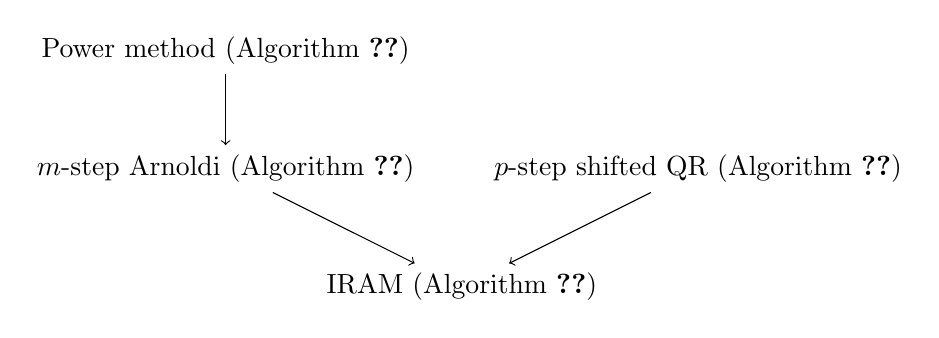
\begin{tikzpicture}
	\node (1) at (0,3) {Power method (Algorithm \ref{Alg:power_method})};
	\node (2) at (0,1.5) {$m$-step Arnoldi (Algorithm \ref{Alg:Arnoldi_iteration})};
	\node (3) at (6,1.5) {$p$-step shifted QR (Algorithm \ref{Alg:shifted_QR_iteration})};
	\node (4) at (3,0) {IRAM (Algorithm \ref{Alg:IRAM})};
	\draw[->] (1) -- (2);
	\draw[->] (2) -- (4);
	\draw[->] (3) -- (4);
\end{tikzpicture}
\caption{Dependency chart for the IRAM.}
\label{Fig:IRAM_flowchart}
\end{figure}

This section follows the treatment found in \cite[Chapters 8, 10]{golub2012matrix}, with occasional minor changes in notation.




\item

The first method we consider is the \textit{power method}, a method for determining the largest magnitude eigenvalue $\lambda_1$ and corresponding eigenvector $v_1$ of a Hermitian matrix $A$.  The power method is based on the property that if $\lambda_1$ is strictly larger in magnitude than the next largest magnitude eigenvalue and the initial vector $q^{(0)}$ has a nonzero component in the direction of $v_1$ (i.e., $v_1^*q^{(0)} \neq 0$), then the sequence
\[
q^{(0)}, \frac{Aq^{(0)}}{||Aq^{(0)}||},  \frac{A^2q^{(0)}}{||A^2q^{(0)}||},  \frac{A^3q^{(0)}}{||A^3q^{(0)}||}, \ldots
\]
will have $v_1$ as its limit.  Formally, the power method is the following algorithm \cite[Section 8.2.1]{golub2012matrix}.


\begin{algorithm}[H]
\caption{Power method}	\label{Alg:power_method}

\begin{algorithmic}[1]
	\Statex 	\textbf{Input:} Hermitian matrix $A$, initial approximate eigenvector $q^{(0)}$, relative tolerance $\textnormal{tol}_\textnormal{rel} > 0$.
	\Statex 	\textbf{Output:} Approximate largest magnitude eigenvalue $\lambda$ and the corresponding eigenvector $v$.
	\State		\textit{Initialize:} $q^{(0)} = q^{(0)}/||q^{(0)}||$, $\rho^{(0)} = [q^{(0)}]^*Aq^{(0)}$, $r^{(0)} = Au^{(0)} - \rho^{(0)}q^{(0)}$, $i= 1$.
	\While {\textit{not converged:} $ ||r^{(i)} || / (||Aq^{(i)}|| + |\rho^{(i)}|) > \textnormal{tol}_\textnormal{rel} $}
		\State		$z^{(i)} = Aq^{(i-1)}$
		\State		$q^{(i)} = z^{(i)} / ||z^{(i)}||$
		\State		$\rho^{(i)} = [q^{(i)}]^* z^{(i)}$
		\State		$r^{(i)} = Aq^{(i)} - \rho^{(i)}q^{(i)}$, $i = i + 1$
	\EndWhile
	\State		\textit{Return:} $(\lambda, v) = (\rho^{(i-1)} , q^{(i-1)})$.
\end{algorithmic}

\end{algorithm}


The simplicity of power method allows for elegant, insightful convergence results like the following theorem, in which we assume the matrix $A$ is real for clarity.

\begin{theorem}			\label{Thm:power_method_conv_rate}
Suppose $A \in \bbR^{n \times n}$ is symmetric with an eigenvalue decomposition
\[
V^*AV = \text{Diag}(\lambda_1, \lambda_2, \ldots, \lambda_n),
\]
where $V = [\ v_1 \ | \ v_2 \ | \cdots | \ v_n \ ]$ is orthogonal and $|\lambda_1| > |\lambda_2| \geq \cdots \geq |\lambda_n|$.  Let the vectors $q^{(i)}$ be generated by Algorithm \ref{Alg:power_method} and define $\theta_i \in [0, \pi/2]$ as 
\[
	\cos(\theta_i) = \left| v_1^Tq^{(i)} \right|.
\]
If $\cos(\theta_0) \neq 0$, then for $i = 0, 1, \ldots$ we have 
\begin{equation} 		\label{Eqn:power_method_conv_rate_1}
\left| \sin(\theta_i) \right| \leq \tan(\theta_0) \left| \frac{\lambda_2}{\lambda_1} \right|^i,
\end{equation}
\begin{equation} 		\label{Eqn:power_method_conv_rate_2}
\left| \lambda^{(i)} - \lambda_1 \right| \leq \max_{2 \leq j \leq n} \left| \lambda_1 - \lambda_i \right| \tan(\theta_0)^2 \left| \frac{\lambda_2}{\lambda_1} \right|^{2i}.
\end{equation}
\end{theorem}

\begin{proof}
See \cite[Theorem 8.2.1]{golub2012matrix}.
\end{proof}

Theorem \ref{Thm:power_method_conv_rate} establishes that the convergence rate of the power method (Algorithm \ref{Alg:power_method}) is dependent on the distance between $|\lambda_1|$ and $|\lambda_2|$.  If this distance $\epsilon = |\lambda_1| - |\lambda_2|$ is very small relative to $|\lambda_1|$, then we have
\[
\left| \frac{\lambda_2}{\lambda_1} \right| = \frac{|\lambda_1| - \epsilon}{|\lambda_1|} = 1 - \frac{\epsilon}{|\lambda_1|} \approx 1,
\]
and $|\sin(\theta_i)|$ in (\ref{Eqn:power_method_conv_rate_1}) may decreases very slowly.  




\item



The next method we consider is the \textit{$m$-step Arnoldi iteration} which extends the power method (Algorithm \ref{Alg:power_method}) to achieve a superior convergence rate.  An iteration of the power method generates a new approximate eigenvector ($q^{(i)}$ from steps 3 and 4) by normalizing the matrix-vector product of the previous vector.  In essence, the power method searches for the largest magnitude eigenvalue $\lambda_1$ and corresponding eigenvector $v_1$ of a matrix $A$ in the one-dimensional subspace $V = \textnormal{span} \{ Aq_1 \}$.  The $m$-step Arnoldi iteration extends the power method by searching for the Ritz pair (\ref{Def:Ritz_pair_val_vec}) ($\theta_1, u_1$) for $A$ with respect to the $m$-dimensional \textit{Krylov subspace}
\begin{equation}
\caK_m(A, q_1) = \textnormal{span}\{ q_1, Aq_1, A^2q_1, \ldots, A^{m-1}q_1 \}.
\label{Def:krylov_subspace}
\end{equation}
Algorithm \ref{Alg:Arnoldi_iteration} (as described in \cite[Algorithm 10.5.1]{golub2012matrix}) builds a unitary basis $Q_m$ of $\caK_m(A, q_1)$ which may be used to find the Ritz pair ($\theta_1, u_1$).
\begin{algorithm}[H]
\caption{$m$-step Arnoldi iteration}	\label{Alg:Arnoldi_iteration}

\begin{algorithmic}[1]
	\Statex		\textbf{Input:} Matrix $A \in \bbC^{n \times n}$, number of Arnoldi steps $m$, initial approximate eigenvector $q_1$.
	\Statex 	\textbf{Output:} Hessenberg matrix $H_m$, basis $Q_m$, residual $r_m$.
	\State		\textit{Initialize:} $q_1  = q_1 / ||q_1||$, \ \ $z = Aq_1$, \ \ $\alpha_1 = q_1^*z$, \ \ $r_1 = z - \alpha_1 q_1$, \ \ $Q_1 = [q_1]$, \ \ $H_1 = [\alpha_1]$.
	\For 			{$i = 1, \ldots, m-1$}
		\State	$\beta_i = ||r_i||$, \ \ $q_{i+1} = r_i / \beta_i$.
		\State	$Q_{i+1} = [Q_i \ | \ q_{i+1}]$, \ \ $\hat{H}_i = \begin{bmatrix}	H_i \\  \beta_i e_i^T	\end{bmatrix}$.
		\State	$z = Aq_{i+1}$.
		\State	$h = Q_{i+1}^*z$, \ \  $r_{i+1} = z - Q_{i+1}h$.
		\State	$H_{i+1} = [\hat{H}_i \ | \ h]$.
	\EndFor
	\State		\textit{Return:} $H_m, Q_m, r_m$.
\end{algorithmic}

\end{algorithm}

In order to obtain a Ritz pair ($\theta, u$) for $A$ with respect to $\caK_m(A, q_1)$, the $m$-step Arnoldi iteration generates an \textit{$m$-step Arnoldi decomposition}
\begin{equation} 		\label{Eqn:Arnoldi_decomp}
AQ_m = Q_m H_m + r_m e_m^*,
\end{equation}
where $H_m$ is an upper Hessenberg matrix.  If $(\theta, w)$ is an eigenpair for $H_m$ and $u = Q_mw$ then (\ref{Eqn:Arnoldi_decomp}) implies
\begin{equation} 			\label{Eqn:Arnoldi_decomp_Ritz_pairs}
(AQ_m - Q_mH_m)w = (A-\theta I) u = (e_m^*w)r_m.
\end{equation}
Additionally, steps 5 and 6 of Algorithm \ref{Alg:Arnoldi_iteration} indicate that $r_m$ is orthogonal to $\caK_m(A, q_1)$, and thus ($\theta, u$) is a Ritz pair for $A$ with respect to $\caK_m(A, q_1)$.  


The use of $\caK_m(A, q_1)$ in Algorithm \ref{Alg:Arnoldi_iteration} allows for superior convergence to Algorithm \ref{Alg:power_method}.  Note that the largest magnitude Ritz pair $(\theta_1, u_1)$ for $A$ with respect to $\caK_m(A, q_1)$ generated by Algorithm \ref{Alg:Arnoldi_iteration}  is guaranteed to be at least comparable to the $m$-th iterate of Algorithm \ref{Alg:power_method} since $A^{m-1}q_1 \in  \caK_m(A, q_1)$.  To compare the convergence rates of Algorithms \ref{Alg:power_method} and \ref{Alg:Arnoldi_iteration} more precisely, assume the matrix $A$ in real and symmetric.  Then the matrix $H_m$ returned by Algorithm \ref{Alg:Arnoldi_iteration} is tridiagonal and this algorithm is equivalent to the \textit{$m$-step Lanczos iteration} \cite[Algorithm 10.1.1]{golub2012matrix}.  In this case, we have the following theorem.  Note that this theorem involves \textit{Chebyshev polynomials} \cite[Section 4.4]{saad2011numerical}, a sequence of polynomials defined recursively as
\begin{equation} 			\label{Def:Chebyshev_polys}
c_k(x) = 2x c_{k-1}(x) - c_{k-2}(x)
\end{equation}
for $k \geq 2$, with $c_0 = 1$ and $c_2 = x$ .

\begin{theorem}   		\label{Thm:Lanczos_conv_rate}
Let $A \in \bbR^{n \times n}$ be symmetric with an eigenvalue decomposition
\[
V^*AV = \text{Diag}(\lambda_1, \lambda_2, \ldots, \lambda_n),
\]
where $V = [\ v_1 \ | \ v_2 \ | \cdots | \ v_n \ ]$ is orthogonal and $\lambda_1 \geq \lambda_2 \geq \cdots \geq \lambda_n$.  Suppose the $m$-step Arnoldi iteration (Algorithm \ref{Alg:Arnoldi_iteration}) is performed and $H_k$ is the tridiagonal matrix returned by this algorithm.  If $\theta_1$ is the largest algebraic eigenvalue of $H_m$, then
\begin{equation} 			\label{Eqn:Lanczos_thm_1}
\lambda_1 \geq \theta_1 \geq \lambda_1 - (\lambda_1 - \lambda_n) 
\left( \frac{\tan(\phi_1)}{c_{m-1}(1+2\rho_1)} \right)^2,
\end{equation}
where $\cos(\phi_1) = |q_1^Tv_1|$,
\begin{equation}		\label{Eqn:Lanczos_thm_2}
\rho_1 = \frac{\lambda_1 - \lambda_2}{\lambda_2 - \lambda_n},
\end{equation}
and $c_{m-1}(x)$ is the Chebyshev polynomial of degree $m-1$.
\end{theorem}

\begin{proof}
See \cite[Theorem 10.1.2]{golub2012matrix}.
\end{proof}

The convergence rate established in Theorem \ref{Thm:Lanczos_conv_rate} may also be applied to Algorithm \ref{Alg:power_method}, giving the following corollary.

\begin{corollary} 			\label{Cor:Lanczos_cor_for_power_method}
Let $A \in \bbR^{n \times n}$ be symmetric and positive semidefinite with an eigenvalue decomposition
\[
V^*AV = \text{Diag}(\lambda_1, \lambda_2, \ldots, \lambda_n),
\]
where $V = [\ v_1 \ | \ v_2 \ | \cdots | \ v_n \ ]$ is orthogonal and $\lambda_1 \geq \lambda_2 \geq \cdots \geq \lambda_n \geq 0$.  Suppose $m$ steps of the power method (Algorithm \ref{Alg:power_method}) are performed and $\gamma_1 = \rho^{(m)}$ is the returned Ritz value.  Then
\begin{equation} 			\label{Eqn:Lanczos_cor_for_power_method}
\lambda_1 \geq \gamma_1 \geq \lambda_1 - (\lambda_1 - \lambda_n) 
\tan^2(\phi_1) \left( \frac{\lambda_2}{\lambda_1} \right)^{2(m-1)},
\end{equation}
where $\cos(\phi_1) = |q_1^Tv_1|$.
\end{corollary}

\begin{proof}
See \cite[Theorem 10.1.2]{golub2012matrix} and replace the Chebyshev polynomial in this proof with $p(x) = x^{k-1}$.
\end{proof}


The lower bounds in Theorem \ref{Thm:Lanczos_conv_rate} and Corollary \ref{Cor:Lanczos_cor_for_power_method} may be used to compare the expected convergence rates for Algorithms \ref{Alg:power_method} and \ref{Alg:Arnoldi_iteration}.  The following comparison is based on \cite[Section 10.1.6]{golub2012matrix}.  Assume $A \in \bbR^{n \times n}$ is symmetric and also positive semidefinite for clarity.  Assume Algorithms \ref{Alg:power_method} and \ref{Alg:Arnoldi_iteration} have been run for $m$ steps with the same initial vector $q_1$.  Let $\gamma_1 = \rho^{(m)}$ be the Ritz value for $A$ generated by step 5 of Algorithm \ref{Alg:power_method}.  And let $\theta_1$ be the Ritz value for $A$ with respect to $\caK_m(A, q_1)$ generated by the largest algebraic eigenvalue of $H_m$ from Algorithm \ref{Alg:Arnoldi_iteration}.  Then we may compare the lower bounds (\ref{Eqn:Lanczos_cor_for_power_method}) for $\gamma_1$ and (\ref{Eqn:Lanczos_thm_1}) for $\theta_1$ by comparing the values
\begin{equation} 		\label{Eqn:power_method_lower_bound}
P_{m-1} = \left( \frac{\lambda_2}{\lambda_1} \right)^{2(m-1)},
\end{equation}
\begin{equation}  	\label{Eqn:Lanczos_lower_bound}
L_{m-1} 
	= \frac{1}{\left[c_{m-1}\left(2\frac{\lambda_1}{\lambda_2} -1 \right)\right]^2} 
	\geq 	\frac{1}{\left[ c_{m-1}\left( 1 + 2 \rho_1 \right) \right]^2}.
\end{equation}
Table \ref{Tab:Lanczos_vs_power_method} compares $P_{m-1}$ and $L_{m-1}$ for a few values of $m$ and $\lambda_1/\lambda_2$.

\begin{table}[H]
\centering
\begin{tabular}{ |c|cc|cc| }
 \hline

 	&	\multicolumn{2}{c|}{$m = 10$}
 		&	\multicolumn{2}{c|}{$m = 20$}	\\
 $\lambda_1 / \lambda_2$	&	$P_{m-1}$	&	$L_{m-1}$
 		&	$P_{m-1}$	&	$L_{m-1}$		\\ 			
 \hline
$1.10$
	&	$1.8 \times 10^{-1}$ & $5.5 \times 10^{-5}$
		&	$2.7 \times 10^{-2}$ & $2.1 \times 10^{-10}$	\\
$1.01$
	&	$8.4 \times 10^{-1}$ & $1.0 \times 10^{-1}$
		&	$6.9 \times 10^{-1}$ & $2.0 \times 10^{-3}$	\\
 \hline
\end{tabular}
\caption{Lower bound terms (\ref{Eqn:power_method_lower_bound}) and (\ref{Eqn:Lanczos_lower_bound}) for Ritz values generated by Algorithms \ref{Alg:power_method} and \ref{Alg:Arnoldi_iteration} } \label{Tab:Lanczos_vs_power_method}
\end{table}

Table \ref{Tab:Lanczos_vs_power_method} demonstrates that the use of the Krylov subspace (\ref{Def:krylov_subspace}) in Algorithm \ref{Alg:Arnoldi_iteration} allows for superior convergence to Algorithm \ref{Alg:power_method}.  Yet this superior convergence rate is slowed somewhat when the desired eigenvalue $\lambda_1$ is close to $\lambda_2$.  For eigenvalue problems where the value $\lambda_1 / \lambda_2$ is very small (like later iterates of the \emep, as demonstrated in Figure \ref{Fig:EMEP_largest_eigvals}), we may seek to increase the number of steps $m$ in Algorithm \ref{Alg:Arnoldi_iteration}.  Yet increasing $m$ can be computationally prohibitive if the eigenvalue problem is very large, requiring significant memory to store $Q_m$ and significant computation to compute the eigenvalue decomposition of $H_m$.




\item

To take advantage of the convergence rate of Algorithm \ref{Alg:Arnoldi_iteration} for larger eigenvalue problems, the Arnoldi decomposition (\ref{Eqn:Arnoldi_decomp}) may be restarted with the \textit{$p$-step shifted QR iteration} developed by \cite{sorensen1992implicit} and discussed in \cite[Sections 10.5.2-3]{golub2012matrix}.  To develop this algorithm, assume we are seeking the $j$ largest eigenvalues of a Hermitian matrix $A \in \bbC^{n \times n}$ and we require that the $m$-step Arnoldi decomposition (\ref{Eqn:Arnoldi_decomp}) $AQ_m = Q_m H_m + r_m e_m^*$ has a fixed size $m > j$.  First we run Algorithm \ref{Alg:Arnoldi_iteration} with the initial vector $q_1$ to obtain $AQ_m = Q_m H_m + r_m e_m^*$.  Next, recall that the matrix $H_m$ may be used to identify the desired Ritz pairs $\{(\theta_i, u_i)\}_{i=1}^j$ for $A$ with respect to $\caK_m(A, q_1)$, as described in (\ref{Eqn:Arnoldi_decomp_Ritz_pairs}).  Yet $H_m$ also contains Ritz values $\theta_{j+1}, \ldots, \theta_m$ which correspond to unwanted eigenvalues of $A$.  To damp these unwanted Ritz values, we may select an appropriate degree $p = m-j$ filter polynomial $p(\lambda)$.  The $p$-step shifted QR iteration uses the filter polynomial
\begin{equation} 			\label{Eqn:filter_poly}
p(\lambda) = c \cdot (\lambda - \mu_1) (\lambda - \mu_2) \cdots (\lambda - \mu_p),
\end{equation}
where $c$ is a constant and the shift values $\mu_1 = \theta_{j+1}, \ldots, \mu_p = \theta_m$ are the $p$ unwanted Ritz values of $A$ with respect to $\caK_m(A, q_1)$.  Algorithm \ref{Alg:shifted_QR_iteration} (as described in \cite[Section 10.5.3]{golub2012matrix}) uses the filter polynomial (\ref{Eqn:filter_poly}) implicitly by applying $p$ shifted QR steps to $H_m$.
%(see \cite[Section 5.2]{golub2012matrix} for details regarding the QR factorization)
\begin{algorithm}[H]
\caption{$p$-step shifted QR iteration (implicit polynomial filtering)}	\label{Alg:shifted_QR_iteration}

\begin{algorithmic}[1]
	\Statex 	\textbf{Input:} Hessenberg matrix $H_m \in \bbC^{m \times m}$ and shift values $\mu_1, \ldots, \mu_p$.
	\Statex 	\textbf{Output:} Processed Hessenberg matrix $H_m^+ \in \bbC^{m \times m}$ and change of basis $V \in \bbC^{m \times m}$, with $H_m^+ = V^*H_mV$.
	\State		Set $H^{(0)} = H_m$.
	\For {$i = 1, \ldots, p$ }
		\State		\textit{QR factorization:} $H^{(i-1)} - \mu_i I = V_iR_i$.
		\State		\textit{Update:} $H^{(i)} = R_iV_i + \mu_iI$.
	\EndFor
	\State		Set $H_m^+ = H^{(p)}$, $V = V_1  V_2 \cdots V_p$.
	\State		\textit{Return:} $H_m^+, V$.
\end{algorithmic}

\end{algorithm}

The following proposition establishes that Algorithm \ref{Alg:shifted_QR_iteration} implicitly applies the filter polynomial $p(\lambda)$ from (\ref{Eqn:filter_poly}) to the initial vector $q_1$ used to create the $m$-step Arnoldi decomposition (\ref{Eqn:Arnoldi_decomp}).

\begin{prop}
Let $A \in \bbC^{n \times n}$ be Hermitian and $AQ_m = Q_mH_m + r_me_m^*$ be the $m$-step Arnoldi decomposition (\ref{Eqn:Arnoldi_decomp}) returned by Algorithm \ref{Alg:Arnoldi_iteration} with initial vector $q_1$.  And let $\mu_1, \ldots, \mu_p$ be the $p$ smallest algebraic eigenvalues of $H_m$.  Run Algorithm \ref{Alg:shifted_QR_iteration} with $H_m$ and $\mu_1, \ldots, \mu_p$ as inputs, and return $H_m^+$, $V = V_1 \cdots V_p$, and $R = R_p \cdots R_1$.

Then the restarted matrix $Q_+ = Q_mV$ will have the first column
\[
q_+ = Q_mV(:,1) = p(A)q_1,
\]
where $p(\lambda)$ is the filter polynomial (\ref{Eqn:filter_poly}) with constant $c = 1/R(1,1)$.
\end{prop}

\begin{proof}
First we must show that 
\begin{equation} 		\label{Eqn:filter_poly_proposition-VR}
VR = (H_m - \mu_1I) \cdots (H_m - \mu_pI).
\end{equation}

Using induction, we see that if $p=1$ then clearly (\ref{Eqn:filter_poly_proposition-VR}) holds.  If $p>1$, then let $\tilde{V}=V_1 \cdots V_{p-1}$ and $\tilde{R} = R_{p-1} \cdots R_1$, and note that $H^{(p-1)} = \tilde{V}^*H_m\tilde{V}$.  Then we have
\[
\begin{split}
VR & = \tilde{V}(V_pR_p)\tilde{R} 
	= \tilde{V} \left( H^{(p-1)} - \mu_pI \right) \tilde{R}
	= \tilde{V}\left( \tilde{V}^*H_m \tilde{V} - \mu_p I \right)\tilde{R}	\\
	& = \left(H_m - \mu_p I \right) \tilde{V}\tilde{R}
	= (H_m - \mu_p I) (H_m - \mu_1 I) \cdots (H_m - \mu_{p-1}I) 	\\
	&=  (H_m - \mu_1I) \cdots (H_m - \mu_pI),
\end{split}
\]
and (\ref{Eqn:filter_poly_proposition-VR}) holds.

Next, note that if the $m$-step Arnoldi decomposition (\ref{Eqn:Arnoldi_decomp}) is right-multiplied by $e_1$, then for all $\mu$ we have
\begin{equation} 			\label{Eqn:filter_poly_propostion-flip}
\left(A - \mu I \right)Q_me_1 = Q_m \left(H_m - \mu I \right) e_1.
\end{equation}

Then we have
\[
\begin{split}
q_+ 
	& = Q_mV(:,1) = Q_m \left[ \frac{1}{R(1,1)}VR e_1 \right] 	\\
	& 	= Q_m p(H_m) e_1 = p(A)Q_m e_1	\\
	& 	= p(A) q_1,
\end{split}
\]
where the third equality is given by (\ref{Eqn:filter_poly_proposition-VR}) and the fourth is given by (\ref{Eqn:filter_poly_propostion-flip}).
\end{proof}


After performing Algorithm \ref{Alg:shifted_QR_iteration}, we have the transformed $m$-step Arnoldi decomposition (\ref{Eqn:Arnoldi_decomp})
\begin{equation}			\label{Eqn:Arnoldi_decomp_transf_shifted_QR}
AQ_+ = Q_+H_+ + r_me_m^*V,
\end{equation}
where $V = V_1 \cdots V_p$ from Algorithm \ref{Alg:shifted_QR_iteration} and $Q_+ = Q_mV$.  As a consequence of the QR steps used in Algorithm \ref{Alg:shifted_QR_iteration}, we can also show that the first $j = m-p$ columns of (\ref{Eqn:Arnoldi_decomp_transf_shifted_QR}) form a new $j$-step Arnoldi decomposition.  Note that $V_1, \ldots, V_p$ are all upper Hessenberg due to the QR factorization in step 3 of Algorithm \ref{Alg:shifted_QR_iteration}.  Then $V$ has a lower band $p$ and $V(m, 1:m-p-1) = V(m, 1:j-1) = 0$, giving
\begin{equation} 			\label{Eqn:Arnoldi_decomp_transf_shifted_QR-part1}
r_me_m^*V(:, 1:j) = V(m,j)r_me_j^*.
\end{equation}
Also, $H_+$ is upper Hessenberg and thus $H_+(j+1:m, 1:j) = H_+(j+1,j)e_1e_j^*$, giving
\begin{equation} 		\label{Eqn:Arnoldi_decomp_transf_shifted_QR-part2}
\begin{split}
Q_+H_+(:, 1:j) 
	&	=  Q_+(:, 1:j) H_+(1:j, 1:j) + Q_+(:, j+1:m)H_+(j+1:m, 1:j) \\
	&	=	Q_+(:, 1:j) H_+(1:j, 1:j) +  H_+(j+1,j)Q_+(:,j+1)e_j^*.
\end{split}
\end{equation}

Therefore, if we set $Q_j = Q_+(:, 1:j) = Q_mV(:, 1:j)$, $H_j = H_+(1:j, 1:j)$, and $r_j = V(m,j)r_m + H_+(j+1,j)Q_+(:,j+1)$, then equations (\ref{Eqn:Arnoldi_decomp_transf_shifted_QR}-\ref{Eqn:Arnoldi_decomp_transf_shifted_QR-part2}) give the new $j$-step Arnoldi decomposition
\begin{equation}		\label{Eqn:Arnoldi_decomp_j-step_update}
\begin{split}
AQ_j  
	&	= AQ_+(:, 1:j) 	\\
	& = Q_+(:, 1:j)H_+(1:j, 1:j) + \left[V(m,j)r_m + H_+(j+1,j)Q_+(:,j+1) \right] e_j^*		\\
	& = Q_jH_j + r_je_j^*,
\end{split}
\end{equation}
and we may resume Algorithm \ref{Alg:Arnoldi_iteration} at step $j+1$.




\item

Combining Algorithms \ref{Alg:Arnoldi_iteration} and \ref{Alg:shifted_QR_iteration} as described above, we have Algorithm \ref{Alg:IRAM} as presented in \cite[Section 10.5.3]{golub2012matrix}.

\begin{algorithm}[H]
\caption{Implicitly restarted Arnoldi method (IRAM)}	\label{Alg:IRAM}

\begin{algorithmic}[1]
	\Statex 	\textbf{Input:} Matrix $A \in \bbC^{n \times n}$, initial approximate eigenvector $q_1$, number of requested largest algebraic eigenvalues $j$, maximum Arnoldi decomposition (\ref{Eqn:Arnoldi_decomp}) size $m$.
	\Statex 	\textbf{Output:} Approximate largest algebraic eigenpairs $(\Lambda_j, V_j)$.
	\State		\textit{Initialize with Algorithm \ref{Alg:Arnoldi_iteration}:} Perform the $m$-step Arnoldi iteration with initial vector $q_1$ to obtain $AQ_m = Q_m H_m + r_m e_m^*$.
	\While {not converged}
		\State		Compute the eigenvalues $\theta_1, \ldots , \theta_m$ of $H_m$ and identify the $p = m-j$ (unwanted) shift values $\mu_1 = \theta_{j+1},  \ldots, \mu_p = \theta_m$.
		\State		\textit{Algorithm \ref{Alg:shifted_QR_iteration}:}  Perform the $p$-step shifted QR iteration to obtain the Hessenberg matrix $H_+$ and change of basis $V$.
		\State		\textit{Restart the Arnoldi factorization:} Set 
		$Q_j = Q_mV(:, 1:j)$,
		$H_j = H_+(1:j, 1:j)$,
		and $r_j = V(m,j)r_m + H_+(j+1,j)Q_+(:,j+1)$ per (\ref{Eqn:Arnoldi_decomp_j-step_update}).
		\State		\textit{Algorithm \ref{Alg:Arnoldi_iteration}:}  Beginning with $AQ_j = Q_jH_j + r_je_j^*$, perform steps $j+1, \ldots, m$ of the Arnoldi iteration to obtain $AQ_m = Q_m H_m + r_m e_m^*$.
	\EndWhile
	\State 		Compute the $j$ largest algebraic eigenvalues $\Lambda_j = \{ \lambda_1, \ldots, \lambda_j\}$ and corresponding eigenvectors $u_1, \ldots, u_j$ of $H_m$.  Set $V_j = [ \ Q_m u_1 \ | \cdots | \ Q_m v_j \ ]$.
	\State		\textit{Return:} $(\Lambda_j, V_j)$.
\end{algorithmic}

\end{algorithm}


The IRAM is one of the two eigenvalue methods we use in Chapter \ref{Sec:Numerics} to handle the \emep.  The choice of parameters $m$ (the Arnoldi decomposition size) and $j$ (number of requested eigenvalues) can greatly impact the efficiency of IRAM (see Section \ref{Subsec:Numerics-adaptive_IRAM}).  For many large-scale eigenvalue problems, the IRAM is a very effective and convenient method.  Due to the implicit polynomial filtering in step 4 of IRAM, this method is particularly effective when the $j$ largest algebraic eigenvalues have modest separation from $\lambda_{j+1}$.  And since the IRAM only has two parameter choices, there is little optimization required by the user.

However, when $\lambda_j \approx \lambda_{j+1}$ and the Arnoldi decomposition size $m$ is not sufficiently large, the IRAM may require many iterations to achieve the desired tolerance.  As we will see in Section \ref{Subsec:Numerics-adaptive_IRAM}, the appropriate choice of $m$ and $j$ in this circumstance may make the IRAM far more competitive.  Yet choosing $m$ and $j$ without prior knowledge of the eigenvalue distribution is inherently heuristic.  Additionally, if the inputted matrix $A$ is very large, then it may be prohibitive to store the $Q_m \in \bbC^{n \times m}$ in active memory.  In particular, if the image or signal $x$ being recovered in the PLGD problem has $n$ pixels, then $Q_m$ will require $m-$times as much storage space.  Thus we proceed in the next section by considering an alternative Krylov subspace method which does not require parameter tuning, nor a large subspace to be held in memory.


Note that the numerical software package \texttt{ARPACK} (the ARnoldi PACKage) is an implementation of IRAM in FORTRAN 77 \cite{lehoucq1998arpack}.  Many numerical computing environments include large-scale eigenvalue methods which having bindings to ARPACK, including \texttt{eigs} in MATLAB, \texttt{eigs} and \texttt{eigsh} in the Python package SciPy, \texttt{eigs} in R, and \texttt{eigs} in the Julia package Arpack.jl. 


\end{enumerate}








\section{The inverse-free preconditioned Krylov subspace method} 	\label{Subsec:evol_mats-eigifp}


\begin{enumerate}


\item



In this section we develop the \textit{inverse-free preconditioned Krylov subspace method} (EIGIFP), another large-scale eigenvalue method which may be used for problems like the \emep.  First proposed by Golub and Ye in \cite{golub2002inverse}, the EIGIFP is a method for solving the \textit{generalized eigenvalue problem} (GEP)
\begin{equation} 			\label{Eqn:GEP}
\begin{array}{ll}
\text{find}	
	&	(\lambda, v) \\
\st
	&	Av = \lambda B v,
\end{array}
\end{equation}
where $A \in \bbC^{n \times n}$ is Hermitian and $B \in \bbC^{n \times n}$ is positive definite.  We say that a pair $(\lambda, v)$ are an \textit{eigenpair of $(A,B)$} if $Av = \lambda Bv$.  Additionally, for a vector $x$, the GEP has the \textit{residual}
\begin{equation} 			\label{Eqn:GEP_residual}
r(x) = \left( A - \frac{x^*Ax}{x^*Bx}  B \right)x,
\end{equation}
where the condition $r(x) = 0$ is equivalent to $(r(x), x)$ being an eigenpair of $(A,B)$.


The EIGIFP has a two-phase algorithmic structure similar to the IRAM (Algorithm \ref{Alg:IRAM}) discussed in the last section.  First, a Krylov subspace (\ref{Def:krylov_subspace}) $\caK$ is formed with Ritz values (\ref{Def:Ritz_pair_val_vec}) for $A$ with respect to $\caK$ which tend to approximate the desired eigenvalues of $A$.  Next, the Ritz values for $A$ with respect to $\caK$ are used to restart the Krylov subspace.  Yet the IRAM and EIGIFP differ in both the choice of Krylov subspace (\ref{Def:krylov_subspace}) and method for restarting this subspace.  

To develop the EIGIFP, we will frame this algorithm as the logical extension of a few more elementary eigenvalue methods.  We begin with the \textit{steepest descent} (SD) method for (\ref{Eqn:GEP}) and show how this method can be extended to the \textit{locally-optimal conjugate gradient} (LOCG) method for (\ref{Eqn:GEP}).  Next, we show that the LOCG method may also be extended to develop the Krylov subspace (\ref{Def:krylov_subspace}) used in EIGIFP.  We also present the \textit{$m$-step Lanczos iteration} for restarting the EIGIFP Krylov subspace, and conclude with the \textit{block inverse-free preconditioned Krylov subspace method} (BLEIGIFP).  Altogether, the algorithms in this section are presented in the following order.

\begin{figure}[H] 
\centering
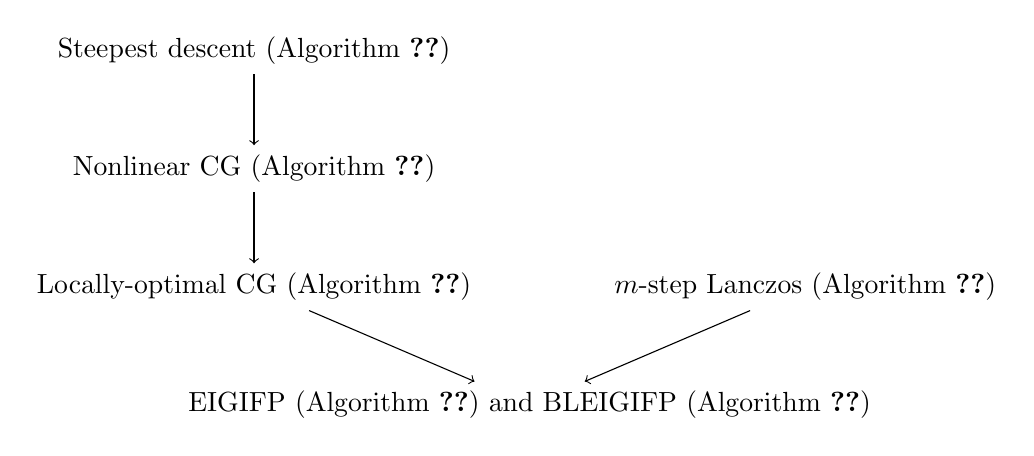
\begin{tikzpicture} 
	\node (1) at (0,4.5) {Steepest descent (Algorithm \ref{Alg:SD})};
	\node (2) at (0,3) {Nonlinear CG (Algorithm \ref{Alg:CG_nonlin})};
	\node (3) at (0,1.5) {Locally-optimal CG (Algorithm \ref{Alg:LOCG})};
	\node (4) at (7,1.5) {$m$-step Lanczos (Algorithm \ref{Alg:eigifp_inner})};
	\node (5) at (3.5,0) {EIGIFP (Algorithm \ref{Alg:eigifp}) and BLEIGIFP (Algorithm \ref{Alg:bleigifp})};
	\draw[->] (1) -- (2);
	\draw[->] (2) -- (3);
	\draw[->] (3) -- (5);
	\draw[->] (4) -- (5);
\end{tikzpicture}
\caption{Dependency chart for the EIGIFP and BLEIGIFP.}
\label{Fig:eigifp_flowchart}
\end{figure}


The Krylov subspace method underlying the EIGIFP was first introduced with a different preconditioning strategy in \cite{knyazev1987convergence}.   We consider the version proposed and analyzed in \cite{golub2002inverse} and implemented based on the technical report \cite{money2005algorithm}.  The BLEIGIFP was first presented in \cite{quillen2010block}.  For a treatment of SD and LOCG methods, the reader may reference \cite{li2015rayleigh}.





\item

We begin by developing the \textit{steepest descent} (SD) method for the GEP (\ref{Eqn:GEP}).  Recall that a steepest descent algorithm involves a function $f(x)$ which is minimized iteratively.  First, an iterate $x$ is used to determine the steepest descent direction $p$ of $f(x)$.  A linesearch is then performed to solve the problem 
\[
\min\limits_{0 < t < \infty} f(x+tp),
\]
and the solution corresponds to a new iterate $x_+$.


To develop a steepest descent algorithm for finding the smallest algebraic eigenvalue of $(A,B)$, we may frame this eigenvalue problem as the \textit{Rayleigh quotient} (RQ) minimization problem
\begin{equation}			\label{Eqn:Rayleigh_quotient_problem}
\min\limits_{x \in \bbR^n} \rho(x) := \frac{x^TAx}{x^TBx},
\end{equation}
where $\rho(x) := {x^TAx}/{x^TBx}$ is the \textit{Rayleigh quotient} (RQ), $A \in \bbR^{n \times n}$ is symmetric, and $B \in \bbR^{n \times n}$ is positive definite.  Note that we define (\ref{Eqn:Rayleigh_quotient_problem}) as a minimization problem to frame the following methods as ``descent'' method.  If $A = -A$, then (\ref{Eqn:Rayleigh_quotient_problem}) will return the largest algebraic eigenvalue of $(A,B)$.

Since $A$ and $B$ in (\ref{Eqn:Rayleigh_quotient_problem}) are real, the RQ has a well-defined gradient
\begin{equation}			\label{Eqn:Rayleigh_gradient}
\nabla \rho(x) = \frac{2}{x^TBx} \left[ Ax - \rho(x)Bx \right]
\end{equation}
and a corresponding steepest descent direction $p := -\nabla \rho(x)$.  Given an iterate $x$ of (\ref{Eqn:Rayleigh_quotient_problem}) and steepest descent direction $p$, we must now perform a linesearch by solving the problem
\begin{equation} 			\label{Eqn:Rayleigh_quotient_linesearch_general}
\min\limits_{0 < t < \infty} \rho(x+tp).
\end{equation}
If $x$ and $p$ are linearly independent, then we may perform an optimal linesearch simply by projecting the problem (\ref{Eqn:Rayleigh_quotient_linesearch_general}) onto the appropriate subspace of $\bbR^n$.  Set $t = \beta/\alpha$, $w = [\alpha; \beta]$, let $Q_1$ be a matrix with orthonormal columns spanning $\{x, p\}$, and set $A_1 = Q_1^TAQ_1$, $B_1 = Q_1^TBQ_1$.  Then we have
\begin{equation} 			\label{Eqn:Rayleigh_linesearch}
\begin{split}
\min\limits_{0 < t < \infty} \rho(x+tp)
	&	 = 			\min\limits_{0 < t < \infty}	\frac{(x+tp)^TA(x+tp)}{(x+tp)^TB(x+tp)}\cdot\frac{\alpha^2}{\alpha^2}\\
	&	 = 		\min\limits_{\alpha, \beta > 0}	\frac{(\alpha x+ \beta p)^TA(\alpha x+\beta p)}{(\alpha x+ \beta p)^TB(\alpha x+ \beta p)} \\
	&	 = 		\min\limits_{\alpha, \beta > 0}		\rho(\alpha x + \beta p)	\\
	&	 = 			\min\limits_{||w|| \neq 0} \frac{w^TA_1w}{w^TB_1w}.
\end{split}
\end{equation}
Finally, note that the steepest descent direction $p = - \nabla \rho(x)$ from (\ref{Eqn:Rayleigh_gradient}) is parallel to the GEP residual (\ref{Eqn:GEP_residual}) $r(x) = Ax - \rho(x)Bx$, and thus we may replace $p$ with $r(x)$ in (\ref{Eqn:Rayleigh_linesearch}).   Then the SD method for the RQ minimization problem (\ref{Eqn:Rayleigh_quotient_problem}) has the following sequence of steps.




\begin{algorithm}[H]
\caption{Steepest descent (SD) method for GEP}	\label{Alg:SD}

\begin{algorithmic}[1]
	\Statex		\textbf{Input:} Matrices $A, B \in \bbR^{n \times n}$ from RQ  problem (\ref{Eqn:Rayleigh_quotient_problem}), initial iterate $x_0$.
	\Statex 	\textbf{Output:} Approximate largest algebraic eigenpair $(\lambda_1, v_1)$.
	\State		\textit{Initialize:} Set $x_0 = x_0/||x_0||$, $r_0 = r(x)$ from (\ref{Eqn:GEP_residual}), $x_{-1} = 0$, $i = 0$.
	\While {not converged}
		\State	$Q_1 = \text{orth}( \{x_i, r_i \} )$.
		\State	$A_1 = Q_1^TAQ_1$, $B_1 = Q_1^TBQ_1$.
%		\State	$w_{i+1} = \text{arg}\min\limits_{||w|| \neq 0} \frac{w^TA_1w}{w^TB_1w}$.
		\State 	Find the largest algebraic eigenpair $(\rho_{i+1}, w_{i+1})$ of $(A_1, B_1)$.
		\State	$x_{i+1} = Q_1w_{i+1}$.
		\State	$r_{i+1} =r(x_{i+1})$ from (\ref{Eqn:GEP_residual}).
		\State 	$i = i + 1$.
	\EndWhile
	\State		\textit{Return:} $\lambda_1 = \rho_i$, $v_1 = x_i$.
\end{algorithmic}

\end{algorithm}



\item



While the SD method (Algorithm \ref{Alg:SD}) is computationally very simple and requires minimal memory, it can also be very slow for ill-conditioned problems, exhibiting the zig-zagging behavior typical of steepest descent algorithms.  This problem may be remedied by extending the search subspace ($Q_1$ from step 3 of Algorithm \ref{Alg:SD}) and thus modifying the search direction.  One choice for a modified search direction is to apply the \textit{nonlinear conjugate gradient} (CG) method \cite{fletcher1964function} to the RQ minimization problem (\ref{Eqn:Rayleigh_quotient_problem}), resulting in the \textit{locally-optimal conjugate gradient} (LOCG) method.  We will briefly review the linear and nonlinear CG methods in order to develop the locally-optimal linesearch strategy used in the LOCG method.



We begin with a brief summary of the \textit{linear cojugate gradient} (CG) method (for a more complete treatment, see \cite[Section 11.3]{golub2012matrix} or \cite[Chapter 5]{nocedal2006numerical}).  First developed in \cite{hestenes1952methods}, the linear CG method is a Krylov subspace method for solving the linear system $Ax = b$, where $A \in \bbR^{n \times n}$ is positive definite and the desired solution is $x_\star := A^{-1}b$.  Since $A$ is positive definite, it induces an \textit{$A$-inner product} and \textit{$A$-norm}, respectively
\begin{equation} 		\label{Eqn:conjugate_inner_product_norm}
\langle x, y \rangle_A := x^TAy, \hspace{1cm} ||x||_A := \sqrt{x^TAx}.
\end{equation}
The linear CG method generates a sequence of iterates $x_i$ which are each optimal in terms of minimizing the function 
\begin{equation}   			\label{Eqn:CG_linear_function}
\phi(x) := \frac{1}{2}||x - x_\star||_A^2 = \frac{1}{2}x^TAx + b^Tx + \frac{1}{2}b^TA^{-1}b
\end{equation}
over the Krylov subspace
\begin{equation}   			\label{Eqn:CG_linear_krylov_subspace}
\caK_i(A,q_1) = \text{span} \left\{q_1, Aq_1, \ldots, A^{i-1}q_1 \right\},
\end{equation}
where $q_1 = b$ if the initial iterate is set to $x_0 = 0$.  Note that $\phi(x)$ is convex and its gradient $\nabla \phi(x) = Ax-b$ is equal to the residual of the system $Ax=b$.  To optimize $\phi(x)$ over $\caK_i(A,b)$, a sequence of search directions $\{p_0, \ldots, p_{n-1}\}$ are created which are \textit{conjugate with respect to $A$}, meaning
\begin{equation} 				\label{Eqn:CG_conj_vectors}
p_i^TAp_j = 0 \ \ \text{for all} \ \ i \neq j.
\end{equation}


An iteration of the linear CG method has the following sequence of steps.  Given a normalized initial iterate $x_0$, the initial residual $r_0 = Ax_0 - b$ is used to create the initial search direction $p_0 = -r_0$, and we set $i=0$.  The function $\phi(x_i + t p_i)$ from (\ref{Eqn:CG_linear_function}) is minimized over $t$.  Setting $\frac{\partial}{\partial t}\phi(x_i + t p_i)$ equal to zero and solving for $t$, we find the closed-form solution
\begin{equation}				\label{Eqn:CG_linear_step_3_orig}
t_i = -\frac{p_i^Tr_i}{p_iAp_i}.
\end{equation}
Next, we update the iterate $x_{i+1} = x_i + t_i p_i$ and residual $r_{i+1} = \nabla \phi (x_{i+1}) = A x_{i+1} - b$.  Finally, we determine a new search direction $p_{i+1}$ which is conjugate to the previous set of search directions.  To satisfy this requirement, we set $p_{i+1} = -r_{i+1} + \beta_i p_i$ and require that
\[
0 = p_i^TAp_{i+1} = p_i^TA( -r_{i+1} + \beta_i p_i),
\]
giving the parameter
\begin{equation}			\label{Eqn:CG_linear_step_6_orig}
\beta_i = \frac{r_{i+1}^TAp_i}{p_iAp_i}.
\end{equation}
This sequence of steps constitutes an iteration of the linear CG method.  Yet equations (\ref{Eqn:CG_linear_step_3_orig}) and (\ref{Eqn:CG_linear_step_6_orig}) may be simplified to arrive at expressions for $t_i$ and $\beta_i$ in common literature (e.g., \cite[Algorithm 11.3.3]{golub2012matrix}, \cite[Algorithm 5.2]{nocedal2006numerical}).
To simplify (\ref{Eqn:CG_linear_step_3_orig}), assume $\beta_{-1} = 0$ and $p_{-1} = 0$.  Then for $i = 0, \ldots, n-1$ we have the search direction update $p_i = -r_i + \beta_{i-1}p_{i-1}$.  Note that $r_i$ is orthogonal to $p_{i-1}$ since $\phi(x_{i-1} + t p_{i-1})$ was minimized along $p_{i-1}$ to find $t_{i-1}$, and then we set $r_i = \nabla \phi(x_{i-1} + t_{i-1} p_{i-1})$.  Then $-p_i^Tr_i = (r_i - \beta_{i-1}p_{i-1})^Tr_i = r_i^Tr_i - \beta_{i-1}p_{i-1}^Tr_i = r_i^Tr_i $, and (\ref{Eqn:CG_linear_step_3_orig}) is equivalent to  
\begin{equation}				\label{Eqn:CG_linear_step_3_in_algo}
t_i = \frac{r_i^Tr_i}{p_iAp_i}.
\end{equation}
To simplify (\ref{Eqn:CG_linear_step_6_orig}), assume $x_0 = 0$.
By construction of the linear CG method,  each iterate $x_{i+1}$ minimizes $\phi$ over $\caK_{i+1}(A, b)$, and thus $r_{i+1} \in \caK_{i+1} (A, b)^{\perp}$.  Since $r_{i} \in \caK_{i+1}(A, b)$, we have 
\begin{equation} 		\label{Eqn:CG_linear_step_3_sub1}
r_{i+1}^Tr_i = 0 \ \ \text{for all} \ \  i = 1, \ldots, n-1.  
\end{equation}
Additionally, note that the update $r_{i+1} = Ax_{i+1} - b = A(x_{i+1} - x_i) + Ax_i - b = t_i Ap_i + r_i$ implies
\begin{equation} 				\label{Eqn:CG_linear_step_3_sub2}
Ap_i = \frac{1}{t_i}(r_{i+1} - r_i).
\end{equation}
Then the numerator in (\ref{Eqn:CG_linear_step_6_orig}) becomes
\begin{equation} 	\label{Eqn:CG_linear_step_3_sub3}
r_{i+1}^TAp_i = \frac{1}{t_i}(r_{i+1} - r_i)^T r_{i+1} = \frac{1}{t_i}r_{i+1}^Tr_{i+1},
\end{equation}
and the denominator in (\ref{Eqn:CG_linear_step_6_orig}) becomes
\begin{equation} 	\label{Eqn:CG_linear_step_3_sub4}
p_i^TAp_i = (-r_i + \beta_{i-1}p_{i-1})^TAp_i = -r_iAp_i = \frac{1}{t_i}r_i^Tr_i.
\end{equation}
And thus (\ref{Eqn:CG_linear_step_6_orig}) simplifies to
\begin{equation}			\label{Eqn:CG_linear_step_6_in_algo}
\beta_i = \frac{r_{i+1}^Tr_{i+1}}{r_i^Tr_i}.
\end{equation}



Altogether, given the steps and simplifications above, we have Algorithm \ref{Alg:CG_linear}.
\begin{algorithm}[H]
\caption{Linear conjugate gradient (CG) method}	\label{Alg:CG_linear}

\begin{algorithmic}[1]
	\Statex		\textbf{Input:} Differentiable function $\phi(x)$, initial iterate $x_0$.
	\Statex 	\textbf{Output:} Solution $x_i$.
	\State		\textit{Initialize:} Set $x_0 = x_0 / ||x_0||$, $r_0 = \nabla \phi (x_0) = Ax_0 - b$, $p_0 = -r_0$, $i = 0$.
	\While {not converged}
		\State	$t_i = \text{arg}\min\limits_{\substack{t}} \phi(x_i + t p_i) = \frac{r_i^Tr_i}{p_iAp_i}$.
		\State	$x_{i+1} = x_i + t_i p_i$.
		\State	$r_{i+1} = \nabla \phi(x_{i+1}) = Ax_{i+1} - b$.
		\State	$\beta_i = \frac{r_{i+1}^Tr_{i+1}}{r_i^Tr_i}$.
		\State	$p_{i+1} = -r_{i+1} + \beta_ip_i$.
		\State 	$i = i + 1$.
	\EndWhile
	\State		\textit{Return:} $x_i$.
\end{algorithmic}

\end{algorithm}



As a consequence of the Cayley-Hamilton theorem \cite[Chapter 12, Proposition 20]{dummit2004abstract}, the linear CG method in exact arithmetic will terminate in $n$ steps, giving $x_{n-1} = x_\star = A^{-1}b \in \caK_{n}(A,b)$ even if $\caK_{n}(A,b) \neq \bbR^n$.  
The Cayley-Hamilton theorem indicates that if $p(\lambda) = \det(\lambda I - A) = \lambda^n + a_1 \lambda^{n-1} + \cdots + a_{n-1}\lambda + a_n$ is the characteristic polynomial of $A$, then $p(A) = A^n + a_1 A^{n-1} + \cdots + a_nI = 0$.  
Then $A^{-1}p(A) = A^{n-1} + a_1 A^{n-2} + \cdots + a_{n-1}I + a_nA^{-1}$, which can be solved for $A^{-1}$ giving
\begin{equation}   	\label{Eqn:CG_linear_conv_prop_1}
x_\star = A^{-1}b =  - \frac{1}{a_n} \left( A^{n-1}b + a_1A^{n-2}b + \cdots + a_{n-1}b \right) \in \caK_{n}(A,b).
\end{equation}
Still assuming exact precision, the linear CG method has the following convergence rate
\begin{equation}		\label{Eqn:CG_linear_conv_prop_2}
\frac{||x_k - x_\star||_A}{||x_\star||_A} \leq 2  \left( \frac{\sqrt{\kappa(A)} - 1}{\sqrt{\kappa(A)} + 1} \right)^k,
\end{equation}
dependent on the condition number $\kappa (A)= \lambda_1 / \lambda_n$ \cite[Theorem 38.5]{trefethen1997numerical}.




We will now consider the \textit{nonlinear CG} method, which seeks to minimize a differentiable function $\phi(x)$.
The nonlinear CG method is nearly identical to the linear CG method (Algorithm \ref{Alg:CG_linear}) except for the absence of conjugate search directions $\{p_i\}_{i=1}^n$.
Recall the linear CG method (Algorithm \ref{Alg:CG_linear}) minimizes the convex quadratic function $\phi(x)$ defined in (\ref{Eqn:CG_linear_function}).  
If instead $\phi(x)$ is not quadratic then this function will not have a fixed positive definite Hessian, and thus any sequence of search directions $\{p_i\}_{i=1}^n$ cannot be conjugate with respect to any inner product.  
Thus the convergence properties (\ref{Eqn:CG_linear_conv_prop_1}) and (\ref{Eqn:CG_linear_conv_prop_2}) will not hold for the nonlinear CG method.  
Despite the lack of convergence guarantees, the nonlinear CG method has been well-studied, and several options exist for choosing the search direction update parameter $\beta_i$ (Algorithm \ref{Alg:CG_linear}, step 6).
The first paper to consider the nonlinear CG method \cite{fletcher1964function} used the parameter
\begin{equation}		\label{Eqn:CG_beta_nonlin1}
\beta_i = \frac{r_{i+1}^Tr_{i+1}}{r_i^Tr_i},
\end{equation} 
where $r_i = \nabla \phi(x_{i+1})$.  The author of \cite{polak1969note} found that the parameter
\begin{equation} 		\label{Eqn:CG_beta_nonlin2}
\beta_i = \frac{r_{i+1}^T(r_{i+1}-r_i)}{r_i^Tr_i}
\end{equation}
had superior performance to (\ref{Eqn:CG_beta_nonlin1}) in some cases.
Given a differentiable function $\phi(x)$ which we seek to minimize and these choices for the search direction update parameter $\beta_i$, we have Algorithm \ref{Alg:CG_nonlin}.


\begin{algorithm}[H]
\caption{Nonlinear conjugate gradient (CG) method}	\label{Alg:CG_nonlin}

\begin{algorithmic}[1]
	\Statex		\textbf{Input:} Differentiable function $\phi(x)$, initial iterate $x_0$.
	\Statex 	\textbf{Output:} Solution $x_i$.
	\State		\textit{Initialize:} Set $x_0 = x_0 / ||x_0||$, $r_0 = \nabla \phi (x_0)$, $p_0 = -r_0$, $i = 0$.
	\While {not converged}
		\State	$t_i = \text{arg}\min\limits_{\substack{t}} \phi(x_i + t p_i)$.
		\State	$x_{i+1} = x_i + t_i p_i$.
		\State	$r_{i+1} = \nabla \phi(x_{i+1})$.
		\State	\textit{Compute conjugate steplength:} $\beta_i$, e.g. (\ref{Eqn:CG_beta_nonlin1}) or (\ref{Eqn:CG_beta_nonlin2}).
		\State	$p_{i+1} = -r_{i+1} + \beta_ip_i$.
		\State 	$i = i + 1$.
	\EndWhile
	\State		\textit{Return:} $x_i$.
\end{algorithmic}

\end{algorithm}

\


xxx here

If $\phi(x) = \rho(x)$ is the Rayleigh quotient of (\ref{Eqn:Rayleigh_quotient_problem}), then the nonlinear CG method seeks to satisfy the nonlinear optimality condition 
\begin{equation}
\nabla \rho(x) = \frac{2}{x^TBx}\left[Ax - \rho(x) Bx \right] = 0.
\end{equation}


Yet when nonlinear CG is applied to the Rayleigh quotient function $\phi(x) = \rho(x)$, the update $x_{i+1}$ may be optimized over both steplengths $t_i$ and $\beta_{i-1}$.  

In the nonlinear CG method, step 4 has the form
\begin{equation}			\label{Eqn:LOCG_spans_optimal_step}
\begin{split}
x_{i+1} \ = 
	& \	x_{i} + t_{i} \left( -r_{i} + \beta_{i-1} p_{i-1} \right) \\
	\in \	&	 \ \text{span} \left\{	x_{i}, r_{i}, p_{i-1}	\right\} 		\\
	= \ 	&	 \ \text{span} \left\{	x_{i}, r_{i}, x_{i-1}	\right\}.
\end{split}
\end{equation}

xxx ABOVE USES: step 7 in Algorithm \ref{Alg:CG_nonlin}, THEN step 4 in same algo

Then if we set $Q_1 = \text{orth}([x_{i-1}, x_i, r_i])$, $A_1 = Q_1^TAQ_1$, and $B_1 = Q_1^TBQ_1$, an argument similar to (\ref{Eqn:Rayleigh_linesearch}) demonstrates that the optimal linesearch for $t_i, \beta_{i-1}$ will be the solution to the problem
\begin{equation}
\min\limits_{||w|| \neq 0} \frac{w^TA_1w}{w^T B_1 w}.
\end{equation}


\


Applying the optimal linesearch for the RQ problem, the nonlinear CG method becomes the locally-optimal conjugate gradient (LOCG) for the RQ problem.  This algorithm can also be viewed as the SD method with the addition of $x_{i-1}$ in the search space.

\begin{algorithm}[H]
\caption{Locally-optimal conjugate gradient (LOCG) for GEP}	\label{Alg:LOCG}

\begin{algorithmic}[1]
	\Statex		\textbf{Input:} Matrices $A, B \in \bbR^{n \times n}$ from RQ  problem (\ref{Eqn:Rayleigh_quotient_problem}), initial iterate $x_0$.
	\Statex 	\textbf{Output:} Approximate largest algebraic eigenpair $(\lambda_1, v_1)$.
	\State		\textit{Initialize:} Set $x_0 = x_0/||x_0||$, $r_0 = r(x_0)$ from  (\ref{Eqn:GEP_residual}), $x_{-1} = 0$, $i = 0$.
	\While {not converged}
		\State	$Q_1 = \text{orth}(\{x_{i-1}, x_i, r_i\})$.
		\State	$A_1 = Q_1^TAQ_1$, $B_1 = Q_1^TBQ_1$.
		\State	Find the largest algebraic eigenpair $(\rho_{i+1}, w_{i+1})$ of $(A_1, B_1)$.
		\State	$x_{i+1} = Q_1w_{i+1}$.
		\State	$r_{i+1} =r(x_{i+1})$ from (\ref{Eqn:GEP_residual}).
		\State 	$i = i + 1$.
	\EndWhile
	\State		\textit{Return:} $\lambda_1 = \rho_i$, $v_1 = x_i$.
\end{algorithmic}

\end{algorithm}





\item


xxx MAKE CLEAR WE JUSTIFY shift-and-invert strategy before stating algo

The inverse-free preconditioned Krylov subspace (eigifp) method extends the SD subspace $Q_1 = \text{span}\{x, (A-\rho B)x\}$ to the Krylov subspace
\begin{equation} 		\label{Eqn:eigifp_Krylov_subspace}
\caK_m(A - \rho B, x) = \text{span} \{ x, (A-\rho B)x, (A-\rho B)^2x, \ldots, (A-\rho B)^{m-1}x \}.
\end{equation}
The choice of this Krylov subspace comes from the effectiveness of shift-and-invert preconditioning strategies for solving eigenvalue problems \cite[Chapter 8]{saad2011numerical}.  To simplify notation, we briefly consider the standard eigenvalue problem.  If $\rho < \lambda_1$ is a current estimate of $\lambda_1$, then we may instead consider the shifted and inverted matrix 
\begin{equation}			\label{Eqn:shift-and-invert-SEP}
C = (A- \rho I)^{-1}.
\end{equation}
The largest algebraic eigenvalue of $C$ will have the form $\theta_1 = 1/(\lambda_1 - \rho)$, so $\rho$ and $\theta_1$ may be used to recover $\lambda_1 = \rho + 1/\theta_1$.  Additionally, if $\rho$ is close to $\lambda_1$, then $\theta_1$ will be very large and the problem of finding $\lambda_1(C)$ may be much better conditioned that the original problem $\lambda_1(A)$.  Also, if $\lambda_2 < \rho < \lambda_1$, then the shifted and inverted eigenvalue problem will have $\theta_1$ as its only positive eigenvalue.

For the GEP, the shifted and inverted matrix
\begin{equation}			\label{Eqn:shift-and-invert-GEP}
C = B(A- \rho B)^{-1}B
\end{equation}
replaces the eigenvalue problem $\lambda_1 = \lambda_1(A,B)$ with $\theta_1 = \lambda_1(C)$.  In this case
\begin{equation}
Cx = \theta_1 Bx  \ \ \ \implies \ \ \  Ax = \left( \rho + \frac{1}{\theta_1} \right) Bx,
\end{equation}
and thus  if $\rho$ is sufficiently close to $\lambda_1$ we again recover $\lambda_1 = \rho + 1/\theta_1$.

If the shift-and-invert technique is used exactly, then the shifted linear system
\begin{equation}
\left( A - \rho B \right) x_+ = Bx
\end{equation}
must be solved directly at each step.  Yet for large eigenvalue problems like the PLGD EMEP, the factorization of $A - \rho B$ is prohibitive and $C-$products must be approximated.  If we use an inverse iteration to approximate $x_+ = CBx = (A-\rho B)^{-1}Bx$, then $x_+$ will be in the subspace $\caK_m(A-\rho B, x)$ for some iterate count $m$.  Eigifp uses this ``inverse-free'' Krylov subspace, applying the corresponding projection to the shifted pencil $(A-\rho B, B)$ and updating $\rho_+ = \rho + 1/\theta_1$.  


While this is theoretically equivalent to projecting $(A,B)$ directly onto $Q_m$, the authors of \cite{golub2002inverse} observe that in practice this saves matrix multiplications by reusing $(A-\rho B)Q_m$ computed in Algorithm \ref{Alg:eigifp_inner} and is also potentially more stable (see \cite[Section 4, Example 1]{golub2002inverse}).




\item

The eigifp method has to main steps: constructing a basis for the Krylov subspace $\caK_m(A-\rho B, x)$ and solving the eigenvalue problem on this subspace to compute eigenpair updates.  Construction of the Krylov subspace is performed with Algorithm \ref{Alg:eigifp_inner}, which is computationally identical to the Arnoldi iteration if the Hessenberg matrix $H_m$ were not formed.


\begin{algorithm}[H]
\caption{$m$-step Lanczos iteration}	\label{Alg:eigifp_inner}

\begin{algorithmic}[1]
	\Statex		\textbf{Input:} Matrix $C \in \bbC^{n \times n}$, number of Lanczos steps $m$, initial approximate eigenvector $q_1$.
	\Statex 	\textbf{Output:} Basis $Q_m$.
	\State		\textit{Initialize:} Set $q_1  = q_1 / ||q_1||$, \ \ $Q_1 = [q_1]$.
	\For 			{$i = 1, \ldots, m-1$}
		\State	$z = Cq_{i}$.
		\State	$h = Q_{i}^*z$, \ \  $r_{i} = z - Q_{i}h$.
		\State	$\beta_i = ||r_i||$, \ \ $q_{i+1} = r_i / \beta_i$.
		\State	$Q_{i+1} = [Q_i \ | \ q_{i+1}]$.
	\EndFor
	\State		\textit{Return:} $Q_m$.
\end{algorithmic}

\end{algorithm}

The Lanczos iteration provides the inner iteration of the single-vector inverse-free preconditioned Krylov subspace method.  Note that step 3 of eigifp includes the previous iterate which we will label $\overline{x}$ in the search space.  This blending of the inverse-free preconditioned Krylov subspace with the CG method has been shown to accelerate the algorithm while adding minimal cost \cite{money2005algorithm}.



\begin{algorithm}[H]
\caption{Inverse-free preconditioned Krylov subspace method (eigifp)}	\label{Alg:eigifp}

\begin{algorithmic}[1]
	\Statex 	\textbf{Input:} Matrices $A, B \in \bbC^{n \times n}$ with $B$ positive definite, initial approximate eigenvector $x_0$, maximum Lanczos basis size $m$,  convergence tolerance $\textnormal{tol}_\textnormal{rel} > 0$.
	\Statex 	\textbf{Output:} Approximate largest algebraic eigenpair $(\lambda_1, v_1)$.
	\State		\textit{Initialize:} Set $x_0 = x_0/||x_0||$, $\rho_0 = x_0^*A x_0 / x_0^* B x_0$, $\overline{x} = 0$, and $i = 0$.
	\While {not converged}
		\State		\textit{Algorithm \ref{Alg:eigifp_inner}:} Perform the $m$-step Lanczos iteration on $C  = A - \rho_i B$ with initial vector $q_1 = x_i$ to obtain $Q_m$.
		\State 		Orthogonalize $\overline{x}$ against $Q_m$ to obtain $q_{m+1}$ and set $\widehat{Q}_m = [Q_m \ | \ q_{m+1}]$.
		\State		Form $A_m = \widehat{Q}_m^*(A-\rho_i B)\widehat{Q}_m$ and $B_m = \widehat{Q}_m^*B \widehat{Q}_m$.
		\State		Compute the largest algebraic eigenpair $(\theta_1, u_1)$ of $(A_m, B_m)$.
		\State		Update $\rho_{i+1} = \rho_i + \theta_1$, $x_{i+1} = \widehat{Q}_m u_1$, $\overline{x} = x_{i+1} - x_i$, and $i = i + 1$.
	\EndWhile
	\State		Set $\lambda_1 = \rho_i$, $v_1 = x_i$.
	\State		\textit{Return:} $(\lambda_1, v_1)$.
\end{algorithmic}

\end{algorithm}

If a preconditioner $L_k$ is provided at iterate $k$, then eigifp only differs in the inner Lanczos iteration.  In this case, the vector $L_kq_1$ is used to construct a Krylov subspace for the transformed eigenvalue problem $(L_k^{-1}AL_k^{-*}, L_k^{-1}BL_k^{-*})$, and then this subspace is premultiplied by $L_k^{-*}$ and orthogonalized to return $Q_m$.  For complete  implementation details, see \cite[Section 5]{golub2002inverse}.  Since the matrix $A$ in the PLGD EMEP is represented implicitly, this preconditioning is not an option.

The PLGD EMEP requires the computation of the two largest algebraic eigenvalues, yet eigifp only computes one eigenvalue at a time.  In order to compute multiple eigenvalues, eigifp is implemented with a deflation strategy.  The basic idea behind deflation is that the $k$ largest algebraic eigenvalues and eigenvectors
\begin{equation}
\Lambda_k = \text{diag}( \lambda_1, \ldots, \lambda_k), \hspace{1cm} V_k = [v_1, \ldots, v_k]
\end{equation}
are used to construct a deflated matrix
\begin{equation}
\widehat{A} = A - V_k \Lambda_k V_k^T.
\end{equation}
Passing $\widehat{A}$ to eigifp will then return $\lambda_1(\widehat{A}) = \lambda_{k+1}$.  Thus eigifp must be called $k$ times to return the $k$ largest algebraic eigenvalues.  Additionally, if these eigenvalues of $A$ are clustered, then this algorithm can converge slowly.  

The typical remedy for these challenges is to replace the single vector iterate in eigifp with a block of vectors.  The resulting block inverse-free preconditioned Krylov subspace method (bleigifp) was developed and analyzed in \cite{quillen2010block}.

\begin{algorithm}[H]
\caption{Block inverse-free preconditioned Krylov subspace method (bleigifp)}	\label{Alg:bleigifp}

\begin{algorithmic}[1]
	\Statex 	\textbf{Input:} Matrices $A, B \in \bbC^{n \times n}$ with $B$ positive definite, initial approximate eigenvectors $Q_j = [q_1, \ldots, q_j]$, maximum Lanczos basis size $m$,  convergence tolerance $\textnormal{tol}_\textnormal{rel} > 0$.
	\Statex 	\textbf{Output:} Approximate largest algebraic eigenpairs $(\Lambda_j, V_j)$.
	\State		\textit{Initialize:} For $i = 1, \ldots, j$, set $q_i = q_i/||q_i||$, $\rho_i = q_i^*A q_i / q_i^* B q_i$, and $\overline{q}_i = 0$.
	\While {not converged}
		\For {$i = 1, \ldots, j$ }
			\State		\textit{Algorithm \ref{Alg:eigifp_inner} with CG step:} Construct a basis $Q^{(i)}$ of $\{\overline{q}_i, \caK_m ( A-\rho_i B , q_i) \}$.
		\EndFor
		\State		Orthonormalize $\left\{ Q^{(1)}, \ldots, Q^{(j)} \right\}$ to obtain $Q_m$.
		\State		Form Krylov subpace problem with $A_m = Q_m^*AQ_m$ and $B_m = Q_m^*B Q_m$.
		\State		Compute the $j$ eigenpairs $(\rho_i, w_i)_{i=1}^j$ of $(A_m, B_m)$.
		\State		Update $\overline{q}_i = q_i$ and $q_i = Q_m w_i$ for $i = 1, \ldots, j$.
	\EndWhile
	\State		Set $\Lambda_j = \text{diag}(\rho_1, \ldots, \rho_j)$, $V_j = [q_1, \ldots, q_j]$.
	\State		\textit{Return:} $(\Lambda_j, V_j)$..
\end{algorithmic}

\end{algorithm}


Black-box implementations of these inverse-free preconditioned Krylov subspace methods are available in MATLAB\footnote{\url{https://www.ms.uky.edu/~qye/software.html}}.  The single-vector implementation \texttt{eigifp} is discussed in \cite{money2005algorithm}, and its block extension \texttt{bleigifp} is discussed in \cite{quillen2010block}.  In the next section, we examine the effectiveness of these methods and IRAM on the PLGD EMEP.


\end{enumerate}


   
   
   

   \chapter{Improved Descent Method and Performance Results}
\label{Sec:Numerics}


\section{Introduction} 		\label{Subsec:Numerics-intro}

In this chapter we present an improved version of Algorithm \ref{Alg:PGD} and examine the performance of this improved algorithm.
Section \ref{Subsec:Numerics-improved_PGD} states the improved version of Algorithm \ref{Alg:PGD}, which applies the new termination conditions of Chapter \ref{Sec:PLGD_term_crit} and \textit{the IRAM with adaptive parameter selection} of Chapter \ref{Sec:evol_mats}.
Next, Section \ref{Subsec:Numerics-perf_results} examines the performance of this improved algorithm.
We demonstrate that this improved algorithm is more efficient than Algorithm \ref{Alg:PGD} for a variety of PLGD models with Gaussian noise (\ref{Eqn:PhaseLift-GD_Gaussian_noise}).
We observe that the improved algorithm often reduces the number of matrix-vector products in the EMEP (\ref{Eqn:EMEP_PLGD}) by at least $50\%$ as compared with Algorithm \ref{Alg:PGD}.
Further experiments show that this reduction in the number of matrix-vector products is comparable 
to the reduction observed by solving the \emep \ with the empirically optimal number of requested eigenvalues for each EMEP iterate.
Finally, we demonstrate that the Arnoldi decomposition (\ref{Eqn:Arnoldi_decomp}) size $m = 40$ for the improved algorithm strikes a proper balance between increasing computational efficiency and minimizing data storage.
Note that all experiments in this chapter involve noisy phase retrieval problems and thus we also use the new termination conditions for Algorithm \ref{Alg:PGD} (otherwise Algorithm \ref{Alg:PGD} would not terminate, as discussed in Section \ref{Subsec:PLGD_term_crit-stagnation}).
All experiments in this chapter are available for reproduction.\footnote{\url{https://github.com/Will-Wright/low-rank-opt-rapid-eig}}






\section{Improved Descent Method}	\label{Subsec:Numerics-improved_PGD}


In this section we briefly summarize the contributions of Chapters \ref{Sec:PLGD_term_crit} and \ref{Sec:evol_mats}.  These contributions lead to an improved version of Algorithm \ref{Alg:PGD}.

Section \ref{Subsec:PLGD_term_crit-stagnation} demonstrated that Algorithm \ref{Alg:PGD} fails to converge for PLGD models with Gaussian noise (\ref{Eqn:PhaseLift-GD_Gaussian_noise}).
Section \ref{Subsec:PLGD_term_crit-new_term_crit} then established new termination conditions: the primal difference condition (\ref{Eqn:term_crit_new-primal_difference}) and the dual variable difference condition (\ref{Eqn:term_crit_new-dual_difference}).
Section \ref{Subsec:PLGD_term_crit-new_term_crit} also demonstrated that these new termination conditions accurately identify stagnation of signal recovery progress in Algorithm \ref{Alg:PGD}.
For convenience, we restate these two new termination conditions:
the primal difference condition
\begin{equation}
	\label{Eqn:term_crit_new-primal_difference2}
\frac{| \rho - \hat{\rho} |}{\rho} \leq  \textnormal{tol}_\textnormal{primal} = 10^{-5}, \ \ \rho = ||\caA(xx^*) - b||_2
\end{equation}
and the dual variable difference condition
\begin{equation}
	\label{Eqn:term_crit_new-dual_difference2}
\frac{||y- \hat{y}||_2}{||y||_2} \leq \textnormal{tol}_\textnormal{dual}= 10^{-4},
\end{equation}
where a hat indicates the previous iterate (e.g., $\hat{y} = y_{k-1}$). 


Section \ref{Subsec:evol_mats-adaptive_IRAM} showed that the computational costs of Algorithm \ref{Alg:PGD} are related to the fixed choice of parameters used in the IRAM (Algorithm \ref{Alg:IRAM}), the eigenvalue method used by Algorithm \ref{Alg:PGD}.
Algorithm \ref{Alg:PGD} uses the IRAM with a fixed the number of requested eigenvalues $r = 2$ and Arnoldi decomposition (\ref{Eqn:Arnoldi_decomp}) size $m = 20$.
Section \ref{Subsec:evol_mats-adaptive_IRAM} examined the empirical performance of the IRAM for a range of parameters $r$ to develop \textit{the IRAM with adaptive parameter selection} (Algorithm \ref{Alg:adaptive_IRAM}).
Algorithm \ref{Alg:adaptive_IRAM} increases $m$ to the default value $40$ and adaptively changes $r$ in order to decrease the number of matrix-vector products required by the IRAM.


Applying these the new termination conditions and Algorithm \ref{Alg:adaptive_IRAM} to Algorithm \ref{Alg:PGD}, we have the improved projected gradient descent algorithm for optimizing the PLGD model (\ref{Eqn:PhaseLift-GD_Gaussian_noise}).

\begin{algorithm}[H]
\caption{Improved projected gradient descent method} 	\label{Alg:PGD-improved}

\begin{algorithmic}[1]
	\Statex 	\textbf{Input:} Sensing operator $\caA$ and adjoint $\caA^*$, observation vector $b$,
	initial dual variable $y_0$, 
	estimate of total noise level $\epsilon$,  
	minimum and maximum number of requested eigenvalues, $r_{min}$ and $r_{max}$, 
	Arnoldi decomposition size $m$,
	and convergence tolerances (\ref{Eqn:term_crit_new-primal_difference2}) and (\ref{Eqn:term_crit_new-dual_difference2}).
	\Statex 	\textbf{Output:} Approximate solution signal $x$.
	\Statex		\textbf{Initialization:} Set $T = \{ \emptyset \}$, $R = \{ \emptyset \}$, $k = 0$.
	\While	{conditions (\ref{Eqn:term_crit_new-primal_difference2}) and (\ref{Eqn:term_crit_new-dual_difference2}) are not satisfied}
		\State 		\textit{Compute algebraically largest eigenvalues and corresponding eigenvectors:} 
		Perform Algorithm \ref{Alg:adaptive_IRAM} with inputs $A_k = \caA^*y_k$, $T$, $R$, $r_{min}$, $r_{max}$, and $m$ to obtain	
		$(\lambda_1, v_1)$, $(\lambda_2, v_2)$, $t_k$, $r_k$.
		\State 		\textit{Compute (sub)gradient:} $g = \caA(v_1 v_1^*)$ based on  (\ref{Eqn:GD-subdifferential}).
		\State		Determine differentiability of $\lambda_1(\caA^*y_k)$ based on (\ref{Eqn:GD-diff_tol}).
		\If {$\lambda_1(\caA^*y_k)$ is differentiable}
			\State		\textit{Linesearch:} Perform linesearch (\ref{Eqn:GD-linesearch}) with initial step $\alpha$ (\ref{Eqn:Barzilai-Borwein_steplength}) to obtain $y_{k+1}$.	
		\Else
			\State		\textit{Projected subgradient step:} Set $y_{k+1} = \Pi_\caC (y_k - \alpha g)$ with $\alpha$ from (\ref{Eqn:GD-steplength_sum}).
		\EndIf
		\State		\textit{Primal recovery:} Compute $\hat{x}$ based on (\ref{Eqn:GD-primal_rec2}).
		\State		\textit{Primal refinement:} Find $x_{k+1}$ as the solution to (\ref{Eqn:GD-PFD}) initialized with $\hat{x}$ and $y_{k+1}$.
		\If {$\epsilon = 0$  } {}
			\State		\textit{Dual refinement:} Find $\widehat{y}$ based on (\ref{Eqn:GD-DFP}).
			\State		\textbf{if} $\lambda_1(\caA^* \widehat{y}) < \lambda_1$, set $y_{k+1} = \widehat{y}$.
		\EndIf
			\State	\textit{Update:} Append $t_k$ to $T$, append $r_k$ to $R$, set $k = k+1$.
	\EndWhile
	\State	\textit{Return:} $x = x_k$. 
\end{algorithmic}

\end{algorithm}


For our implementation of Algorithm \ref{Alg:PGD-improved}, we use the default values $r_{min}=2$, $r_{max} = \min\{ 30, m-5 \}$, and $m=40$ (as discussed in Section \ref{Subsec:evol_mats-adaptive_IRAM}).




\section{Performance Results} 		\label{Subsec:Numerics-perf_results}


We now examine the performance behavior of Algorithm \ref{Alg:PGD-improved} for a variety of noisy phase retrieval problems.

First, we compare the performance of Algorithm \ref{Alg:PGD} and Algorithm \ref{Alg:PGD-improved} for a variety of randomly generated and image-based phase retrieval problems.
Figure \ref{Fig:Numerics-ada_vs_orig_various_params} depicts a set of experiments with randomly generated signals.


\begin{figure}[H]
\centering
\hbox{\hspace{-1.1cm} 
	\includegraphics[scale=0.6]{Numerics-ada_vs_orig_various_params}
			}
	\vspace{0.0cm}
	\caption{
	Performance results for PLGD models with Gaussian noise (\ref{Eqn:PhaseLift-GD_Gaussian_noise}), where signals are complex with standard Gaussian distribution (\ref{Def:Gaussian_distribution_complex}).
	Results indicate Algorithm \ref{Alg:PGD} (solid line) and Algorithm \ref{Alg:PGD-improved} (dashed line). 
	Each result is the mean of 10 experiments.
	Left: Varying signal size $n$, with fixed noise ratio $\epsilon_\text{rel} = 0.15$ and oversampling scaled logarithmically with $n$ (i.e., $L = 10, 12, 12, 14$) as indicated in Theorem \ref{Thm:PhaseLift_approx}.
	Middle: Varying oversampling rate $L$, with fixed signal size $n = 128$ and noise ratio $\epsilon_\text{rel} = 0.15$.
	Right: Varying noise ratio $\epsilon_\text{rel}$, with fixed signal size $n = 128$ and oversampling rate $L = 10$.
	}
\label{Fig:Numerics-ada_vs_orig_various_params}
\end{figure}
% experiments.figure.noisyimage_comparison_adaptive_vs_orig

Figure \ref{Fig:Numerics-ada_vs_orig_various_params} demonstrates that Algorithm \ref{Alg:PGD-improved} requires fewer matrix-vector products than Algorithm \ref{Alg:PGD} for a wide range of phase retrieval problems.
The left and middle plots in Figure \ref{Fig:Numerics-ada_vs_orig_various_params} suggest that Algorithm \ref{Alg:PGD-improved} requires about $60\%$ fewer matrix-vector products regardless of signal size $n$ or oversampling rate $L$.
Additionally, the right plot in Figure \ref{Fig:Numerics-ada_vs_orig_various_params} suggests Algorithm \ref{Alg:PGD-improved} may reduce matrix-vector products by $80\%$ or more for problems with significant noise.


We also find that Algorithm \ref{Alg:PGD-improved} is more efficient than Algorithm \ref{Alg:PGD} for image-based phase retrieval problems.
Table \ref{Tab:Numerics-ada_vs_orig_large_images} shows the performance results for two larger images from Figure \ref{Fig:Numerics-large_images}.



\begin{table}[H]
\centering
\begin{tabular}{ |ccc|c|cc|cc| }
 \hline
			&&&  Algorithm \ref{Alg:PGD}
			&  \multicolumn{2}{c|}{Algorithm \ref{Alg:PGD-improved}}
			&	\multicolumn{2}{c|}{Algorithm \ref{Alg:PGD-improved}}	\\
Image & $n$ & $L$ &  	& \multicolumn{2}{c|}{$m=40$}  & \multicolumn{2}{c|}{$m=80$}   \\
 \hline
	\multirow{2}{*}{Figure \ref{Fig:Numerics-large_images}, left} &
   \multirow{2}{*}{$57,600$} &  10 &  562,255  &  297,767 & 47\% &  252,316 & 55\% \\ 
  &&  15 &  647,753  &  301,752 & 53\% &  253,209 & 61\% \\ 
	\multirow{2}{*}{Figure \ref{Fig:Numerics-large_images}, right}  &   
     \multirow{2}{*}{$120,000$} &  10 &  852,633  &  364,164 & 57\% &  287,309 & 66\% \\ 
  &&  15 &  563,085  &  291,630 & 48\% &  256,084 & 55\% \\ 
 \hline
\end{tabular}
\caption{
Performance results for PLGD models with Gaussian noise (\ref{Eqn:PhaseLift-GD_Gaussian_noise}), where signals are the images in Figure \ref{Fig:Numerics-large_images}.
Results indicate total number of matrix-vector products and percent decrease from Algorithm \ref{Alg:PGD}.
Parameter $m$ is the Arnoldi decomposition size (\ref{Eqn:Arnoldi_decomp}) for the IRAM (Algorithm \ref{Alg:IRAM}).
	} 
	\label{Tab:Numerics-ada_vs_orig_large_images}
\end{table}
% experiments.figure.noisyimage_comparison_adaptive_vs_orig



\begin{figure}[H]
\centering
	\includegraphics[scale=0.46875]{jul_and_me_orig}
		\hspace{0.1cm}
		\includegraphics[scale=0.5625]{UCD_orig}
		\vspace{0.3cm} \hspace{0.02cm}
		\\
	\includegraphics[scale=0.46875]{jul_and_me_L_15_ada40}	
		\hspace{0.1cm}
		\includegraphics[scale=0.5625]{UCD_L_15_ada40} 
		\vspace{0.0cm}
	\caption{
Images used for experiments in Table \ref{Tab:Numerics-ada_vs_orig_large_images}.
Top left: original image of my daughter and me, image size $240 \times 240 = 57,600$ pixels.
Bottom left: result image after solving EMEP.
Top right: original image of UC Davis roundabout, image size $200 \times 600 = 120,000$ pixels.
Bottom right: result image after solving EMEP.
All experiments have noise ratio $\epsilon_\text{rel} = 0.15$ and oversampling $L = 15$.
	}
\label{Fig:Numerics-large_images}
\end{figure}
% experiments.figure.noisyimage_comparison_adaptive_vs_orig


Table \ref{Tab:Numerics-ada_vs_orig_large_images} demonstrates that the benefits of Algorithm \ref{Alg:PGD-improved} also apply to large-scale phase retrieval problems.
Additionally, a larger Arnoldi decomposition size $m$ further reduces the number of matrix-vector products.
Thus, when solving large-scale problems it may be advisable to consider increasing this parameter beyond the default setting of $m=40$ in Algorithm \ref{Alg:PGD-improved} if memory constraints permit this increase.




Next, we demonstrate that the computational performance improvements of Algorithm \ref{Alg:PGD-improved} are comparable to the improvements of solving the \emep \ with the empirically optimal value $\bar{r}_k$ for each EMEP iterate $k$.
Table \ref{Tab:Numerics-num_matvecs_opt_vs_ada} indicates the number of matrix-vector products for six PLGD models with Gaussian noise (\ref{Eqn:PhaseLift-GD_Gaussian_noise}) using Algorithm \ref{Alg:PGD} ($r=2$), Algorithm \ref{Alg:PGD-improved} ($r$ chosen with Algorithm \ref{Alg:adaptive_IRAM}), and the empirically optimal sequence of values $\bar{r}_k$.



\begin{table}[H]
\centering
\begin{tabular}{ |ccc|c|cc|cc| }
 \hline
			&&&  Algorithm \ref{Alg:PGD}
			&	\multicolumn{2}{c|}{Algorithm \ref{Alg:PGD-improved}  }
			&  \multicolumn{2}{c|}{ Empirically optimal $\bar{r}$ }	\\
$L$ & $\epsilon_\text{rel}$ & EMEP its &  	& \multicolumn{2}{c|}{ $m=40$ }  & \multicolumn{2}{c|}{$m=40$}   \\
 \hline
 5 &  0.05 & 300 &  406,308  &  198,070 & 51\% &  179,807 & 56\%  \\ 
  5 &  0.15 & 300 & 1,099,045  &  258,385 & 76\% &  242,003 & 78\%  \\ 
  5 &  0.30 &  92 &  444,697  &   69,510 & 84\% &   58,780 & 87\%  \\ 
 10 &  0.05 & 153 &   80,453  &   68,709 & 15\% &   61,948 & 23\%  \\ 
 10 &  0.15 & 108 &   88,317  &   57,231 & 35\% &   51,311 & 42\%  \\ 
 10 &  0.30 &  54 &   72,486  &   25,809 & 64\% &   23,217 & 68\%  \\ 
 \hline
\end{tabular}

\caption{
Performance results for PLGD models with Gaussian noise (\ref{Eqn:PhaseLift-GD_Gaussian_noise}) with original signal from Figure \ref{Fig:parrot_signal_iterates} resized to $64 \times 64$ pixels.
Results indicate total number of matrix-vector products and percent decrease from Algorithm \ref{Alg:PGD}.
Parameter $m$ is the Arnoldi decomposition size (\ref{Eqn:Arnoldi_decomp}).
} \label{Tab:Numerics-num_matvecs_opt_vs_ada}
\end{table}
% experiments.figure.noisyimage_adaptive_eig_full_exp


For each of the experiments in Table \ref{Tab:Numerics-num_matvecs_opt_vs_ada}, we see that Algorithm \ref{Alg:PGD-improved} offers nearly the same performance improvement as that of solving the EMEP with the empirically optimal values $\bar{r}_k$.
Notably, experiments in Table \ref{Tab:Numerics-num_matvecs_opt_vs_ada} with a low oversampling rate ($L=5$) shows that Algorithm \ref{Alg:PGD-improved} is particularly effective at decreasing the number of matrix-vector products when there is a large relative difference between the number of matrix-vector products for Algorithm \ref{Alg:PGD} and the empirically optimal choice of values $\bar{r}_k$.
To further explore this performance behavior, Figure \ref{Fig:Numerics-num_eigs_ada_vs_opt} depicts the two PLGD models from Table \ref{Tab:Numerics-num_matvecs_opt_vs_ada} with the largest and smallest relative difference in matrix-vector products (those with $L=5$, $\epsilon_\text{rel} = 0.15$, and $L=10$, $\epsilon_\text{rel} = 0.05$, respectively).




\begin{figure}[H]
\centering
\hbox{\hspace{-1.0cm} \includegraphics[scale=0.6]{Numerics-num_eigs_ada_vs_opt_1} }\vspace{0.6cm}
\hbox{\hspace{-1.0cm} \includegraphics[scale=0.6]{Numerics-num_eigs_ada_vs_opt_2} }
\vspace{0.2cm}
	\caption{
	Number of requested eigenvalues $r$ in the IRAM (Algorithm \ref{Alg:IRAM}) for two PLGD models from Table \ref{Tab:Numerics-num_matvecs_opt_vs_ada}.
	}
\label{Fig:Numerics-num_eigs_ada_vs_opt}
\end{figure}
% experiments.figure.noisyimage_adaptive_eig_full_exp


In both PLGD models depicted in Figure \ref{Fig:Numerics-num_eigs_ada_vs_opt}, the number of requested eigenvalues $r$ selected by Algorithm \ref{Alg:PGD-improved} is usually within 1-3 units from the empirically optimal value $\bar{r}$.
The bottom plot in Figure \ref{Fig:Numerics-num_eigs_ada_vs_opt} suggests that Algorithm \ref{Alg:PGD-improved} required relatively more matrix-vector products than the empirically optimal value $\bar{r}$ because the subroutine Algorithm \ref{Alg:adaptive_IRAM} used in Algorithm \ref{Alg:PGD-improved} always changes the value of $r$ by one or two units, thus shifting away from the optimal value $\bar{r}=2$ for many EMEP iterates.
As we saw in Section \ref{Subsec:evol_mats-adaptive_IRAM} (e.g., Figure \ref{Fig:Numerics-surf_mvs_eig_diffs_2}) the empirically optimal value $\bar{r}$ may shift rapidly for some PLGD models, and thus Algorithm \ref{Alg:adaptive_IRAM} always changes $r$ by one or two units to continue gathering performance information about the EMEP.




Finally, we consider another set of performance results to justify selecting $m=40$ as the default Arnoldi decomposition (\ref{Eqn:Arnoldi_decomp}) size for Algorithm \ref{Alg:PGD-improved}.
Table \ref{Tab:Numerics-num_matvecs_orig_vs_ada} depicts the total number of matrix-vector products required to solve the \emep \ for each PLGD model from Table \ref{Tab:Numerics-num_matvecs_opt_vs_ada} with Algorithm \ref{Alg:PGD-improved} with various parameter values $m$.

\begin{table}[H]
\centering
\begin{tabular}{ |ccc|c|ccccc| }
 \hline
			  \multicolumn{3}{|c|}{n = 4,096} & Algorithm \ref{Alg:PGD}
			&  \multicolumn{5}{c|}{Algorithm \ref{Alg:PGD-improved}}	\\
$L$ & $\epsilon_\text{rel}$ & EMEP its & 	& $m=20$  & $m=40$  & $m=60$  & $m=80$  & $m=100$   \\
 \hline
  5 &  0.05 & 300 &  406,308  &  358,195  &  198,070  &  189,401  &  192,042  &  201,270  \\ 
  5 &  0.15 & 300 & 1,099,045  &  806,412  &  258,385  &  224,048  &  214,118  &  215,392  \\ 
  5 &  0.30 &  92 &  444,697  &  175,669  &   69,510  &   56,193  &   55,146  &   54,987  \\ 
 10 &  0.05 & 153 &   80,453  &   77,768  &   68,709  &   64,300  &   68,602  &   73,754  \\ 
 10 &  0.15 & 108 &   88,317  &   65,833  &   57,231  &   53,261  &   54,388  &   55,308  \\ 
 10 &  0.30 &  54 &   72,486  &   28,799  &   25,809  &   24,699  &   25,113  &   25,491  \\ 
 \hline
\end{tabular}

\caption{
Total number of matrix-vector products for various PLGD models with Gaussian noise	(\ref{Eqn:PhaseLift-GD_Gaussian_noise}) with original signal from Figure \ref{Fig:parrot_signal_iterates} resized to $64 \times 64$ pixels.
Parameter $r$ is the number of requested eigenvalues in the IRAM (Algorithm \ref{Alg:IRAM}) and $m$ is the Arnoldi decomposition (\ref{Eqn:Arnoldi_decomp}) size. 
} \label{Tab:Numerics-num_matvecs_orig_vs_ada}
\end{table}
% experiments.figure.noisyimage_adaptive_eig_full_exp



Table \ref{Tab:Numerics-num_matvecs_orig_vs_ada} demonstrates that Algorithm \ref{Alg:PGD-improved} reduces the number of matrix-vector products from those of Algorithm \ref{Alg:PGD} for all experiments considered.
Yet this cost reduction varies significantly depending on the choice of Arnoldi decomposition (\ref{Eqn:Arnoldi_decomp}) size $m$.
We seek a default setting for the parameter $m$ which is sufficiently large to yield the benefits of Algorithm \ref{Alg:PGD-improved}, yet sufficiently small as not to impact memory constraints.
To select an appropriate default value for $m$, we examine the two experiments from Table \ref{Tab:Numerics-num_matvecs_orig_vs_ada} with $\epsilon_\text{rel} = 0.15, 0.30$ and $L=5$ which have the greatest original number of matrix-vector products, along with the greatest total decrease in cost when using Algorithm \ref{Alg:PGD-improved} with a sufficiently large parameter $m$.
Figure \ref{Fig:Numerics-num_matvecs_ada_for_m_vals} singles out these two experiments, depicting the number of matrix-vector products for each \emep \ iteration.

\begin{figure}[H]
\centering
\hbox{\hspace{-0.9cm} \includegraphics[scale=0.6]{Numerics-num_matvecs_ada_for_m_vals} }\vspace{0.0cm}
	\caption{Number of matrix-vector products for each \emep \ iteration from two experiments in Figure \ref{Fig:Numerics-num_matvecs_ada_for_m_vals} with various Arnoldi decomposition size $m=20, 40, 80$.}
\label{Fig:Numerics-num_matvecs_ada_for_m_vals}
\end{figure}
% experiments.figure.noisyimage_adaptive_eig_full_exp




Figure \ref{Fig:Numerics-num_matvecs_ada_for_m_vals} demonstrates that the Arnoldi decomposition size of $m=20$ is not sufficiently large to allow Algorithm \ref{Alg:PGD-improved} to decrease the number of matrix-vector products.  
The dramatic matrix-vector product spikes for $m=20$ in Figure \ref{Fig:Numerics-num_matvecs_ada_for_m_vals} resemble those first seen in Figure \ref{Fig:EMEP_costs_num_mat_vecs} when using Algorithm \ref{Alg:PGD}.
Yet when the Arnoldi decomposition size is increased to $m=40$, these cost spikes effectively disappear.
The change in number of matrix-vector products between $m=40$ and $m=80$ is minimal for each EMEP iterate.  
Thus the default parameter of $m=40$ for Algorithm \ref{Alg:PGD-improved} strikes the proper balance between efficiency and memory constraints.












         
   
   
	\chapter{Conclusion}			\label{Sec:Conclusion}


In this chapter we conclude our work on the PLGD model (\ref{Eqn:PhaseLift-P-GD}) and the \emep.
Section \ref{Subsec:Conclusion-performance_results} demonstrates the effectiveness of the IRAM with adaptive parameter selection (Algorithm \ref{Alg:adaptive_IRAM}) for a variety of noisy phase retrieval problems.
Section \ref{Subsec:Conclusion-contrib_and_future} summarizes the contributions made in this dissertation and suggests possible future work.



\section{Performance results} 			\label{Subsec:Conclusion-performance_results}


This section demonstrates the efficiency of the IRAM with adaptive parameter selection (Algorithm \ref{Alg:adaptive_IRAM}) for solving the \emep.
We begin by demonstrating that Algorithm \ref{Alg:adaptive_IRAM} is more efficient than the original IRAM (Algorithm \ref{Alg:IRAM}) parameter settings for a variety of PLGD models with Gaussian noise (\ref{Eqn:PhaseLift-GD_Gaussian_noise}).
We observe that Algorithm \ref{Alg:adaptive_IRAM} typically reduces the number of matrix-vector products in the EMEP by at least $50\%$ as compared with the original IRAM settings.
Next, we show that Algorithm \ref{Alg:adaptive_IRAM} is nearly optimal as a method for choosing the ideal number of requested eigenvalues $r_k$ corresponding to the minimum number of matrix-vector products necessary for each EMEP iteration.
Finally, we demonstrate that the Arnoldi decomposition (\ref{Eqn:Arnoldi_decomp}) size parameter $m = 40$ for Algorithm \ref{Alg:adaptive_IRAM} strikes a proper balance between increasing computational efficiency and minimizing data storage.
Note that all experiments in this section are performed using termination conditions (\ref{Eqn:term_crit_new-primal_difference}) and (\ref{Eqn:term_crit_new-dual_difference}) established in Chapter \ref{Sec:PLGD_term_crit}.
All experiments are available for reproduction.\footnote{\url{https://github.com/Will-Wright/low-rank-opt-rapid-eig}}


%\subsection{Performance results for two EMEP methods}  			\label{Subsubsec:Conclusion-gen_perf_results}


We begin by comparing the performance of Algorithm \ref{Alg:adaptive_IRAM} and the original IRAM parameter choices for a variety of randomly generated and image-based phase retrieval problems.
Figure \ref{Fig:Numerics-ada_vs_orig_various_params} depicts a set of experiments with randomly generated signals.


\begin{figure}[H]
\centering
\hbox{\hspace{-1.8cm} 
	\includegraphics[scale=0.6]{Numerics-ada_vs_orig_various_params}
			}
	\vspace{0.0cm}
	\caption{
	Performance results for PLGD models with Gaussian noise (\ref{Eqn:PhaseLift-GD_Gaussian_noise}), where signals are complex with standard Gaussian distribution (\ref{Def:Gaussian_distribution_complex}).
	Results indicate Algorithm \ref{Alg:adaptive_IRAM} (dashed line) and the original IRAM parameters $m=20$, $r = 2$ (solid line). 
	Each result is the mean of 10 experiments.
	Left: Varying signal size $n$, with fixed noise ratio $\epsilon_\text{rel} = 0.15$ and oversampling scaled logarithmically with $n$ (i.e., $L = 10, 12, 12, 14$) as indicated in Theorem \ref{Thm:PhaseLift_approx}.
	Middle: Varying oversampling rate $L$, with fixed signal size $n = 128$ and noise ratio $\epsilon_\text{rel} = 0.15$.
	Right: Varying noise ratio $\epsilon_\text{rel}$, with fixed signal size $n = 128$ and oversampling rate $L = 10$.
	}
\label{Fig:Numerics-ada_vs_orig_various_params}
\end{figure}
% experiments.figure.noisyimage_comparison_adaptive_vs_orig

Figure \ref{Fig:Numerics-ada_vs_orig_various_params} demonstrates that Algorithm \ref{Alg:adaptive_IRAM} requires fewer matrix-vector products than the original IRAM parameters for the \emep \ for a wide range of phase retrieval problems.
The left and middle plots in Figure \ref{Fig:Numerics-ada_vs_orig_various_params} suggest that Algorithm \ref{Alg:adaptive_IRAM} requires about $60\%$ fewer matrix-vector products regardless of signal size $n$ or oversampling rate $L$.
Additionally, the right plot in Figure \ref{Fig:Numerics-ada_vs_orig_various_params} suggests Algorithm \ref{Alg:adaptive_IRAM} may reduce matrix-vector products by $80\%$ or more for problems with significant noise.


We also find that Algorithm \ref{Alg:adaptive_IRAM} is more efficient than the original IRAM settings for image-based phase retrieval problems.
Table \ref{Tab:Numerics-ada_vs_orig_large_images} shows the performance results for two larger images from Figure \ref{Fig:Numerics-large_images}.



\begin{table}[H]
\centering
\begin{tabular}{ |ccc|c|cc|cc| }
 \hline
			&&&  Original
			&  \multicolumn{2}{c|}{Algorithm \ref{Alg:adaptive_IRAM}}
			&	\multicolumn{2}{c|}{Algorithm \ref{Alg:adaptive_IRAM}}	\\
Image & $n$ & $L$ & $r=2, m=20$	& \multicolumn{2}{c|}{$m=40$}  & \multicolumn{2}{c|}{$m=80$}   \\
 \hline
	\multirow{2}{*}{Figure \ref{Fig:Numerics-large_images}, left} &
   \multirow{2}{*}{$57,600$} &  10 &  562,255  &  297,767 & 47\% &  252,316 & 55\% \\ 
  &&  15 &  647,753  &  301,752 & 53\% &  253,209 & 61\% \\ 
	\multirow{2}{*}{Figure \ref{Fig:Numerics-large_images}, right}  &   
     \multirow{2}{*}{$120,000$} &  10 &  852,633  &  364,164 & 57\% &  287,309 & 66\% \\ 
  &&  15 &  563,085  &  291,630 & 48\% &  256,084 & 55\% \\ 
 \hline
\end{tabular}
\caption{
Performance results for PLGD models with Gaussian noise (\ref{Eqn:PhaseLift-GD_Gaussian_noise}), where signals are the images in Figure \ref{Fig:Numerics-large_images}.
Results indicate total number of matrix-vector products and percent decrease from the original IRAM parameters.
Parameter $r$ is the number of requested eigenvalues in the IRAM (Algorithm \ref{Alg:IRAM}) and $m$ is the Arnoldi decomposition size (\ref{Eqn:Arnoldi_decomp}).
	} 
	\label{Tab:Numerics-ada_vs_orig_large_images}
\end{table}
% experiments.figure.noisyimage_comparison_adaptive_vs_orig



\begin{figure}[H]
\centering
	\includegraphics[scale=0.4166666666]{jul_and_me_orig}
		\hspace{0.1cm}
		\includegraphics[scale=0.5]{UCD_orig}
		\vspace{0.3cm} \hspace{0.02cm}
		\\
	\includegraphics[scale=0.4166666666]{jul_and_me_L_15_ada40}	
		\hspace{0.1cm}
		\includegraphics[scale=0.5]{UCD_L_15_ada40} 
		\vspace{0.0cm}
	\caption{
Images used for experiments in Table \ref{Tab:Numerics-ada_vs_orig_large_images}.
Top left: original image of my daughter and me, image size $240 \times 240 = 57,600$ pixels.
Bottom left: result image after solving EMEP.
Top right: original image of UC Davis roundabout, image size $200 \times 600 = 120,000$ pixels.
Bottom right: result image after solving EMEP.
All experiments have noise ratio $\epsilon_\text{rel} = 0.15$ and oversampling $L = 15$.
	}
\label{Fig:Numerics-large_images}
\end{figure}
% experiments.figure.noisyimage_comparison_adaptive_vs_orig


Table \ref{Tab:Numerics-ada_vs_orig_large_images} demonstrates that the benefits of Algorithm \ref{Alg:adaptive_IRAM} also apply to large-scale phase retrieval problems.
Additionally, a larger Arnoldi decomposition size $m$ further reduces the number of matrix-vector products.
Thus, when solving large-scale problems it may be advisable to consider increasing this parameter beyond the default setting of $m=40$ in Algorithm \ref{Alg:adaptive_IRAM} if memory constraints permit this increase.



Next, we demonstrate that Algorithm \ref{Alg:adaptive_IRAM} is nearly optimal in the sense of choosing the number of requested eigenvalues $r_k$ which minimizes the number of matrix-vector products for each \emep \ iterate $k$.
Table \ref{Tab:Numerics-num_matvecs_opt_vs_ada} indicates the number of matrix-vector products for solving the EMEP for six PLGD models with Gaussian noise (\ref{Eqn:PhaseLift-GD_Gaussian_noise}) with Algorithm \ref{Alg:adaptive_IRAM}, with the original IRAM parameters, and with the minimum possible number of matrix-vector products if each value $r_k$ was chosen such that $2 \leq r_k\leq 30$ and $r_k$ corresponds to the minimum number of matrix-vector products for the IRAM to evaluate EMEP iterate $k$.


\begin{table}[H]
\centering
\begin{tabular}{ |ccc|c|cc|cc| }
 \hline
			&&&  Original
			&  \multicolumn{2}{c|}{Optimal $2 \leq r \leq 30$}
			&	\multicolumn{2}{c|}{Algorithm \ref{Alg:adaptive_IRAM}}	\\
$L$ & $\epsilon_\text{rel}$ & EMEP its & $r=2, m=20$	& \multicolumn{2}{c|}{$m=40$}  & \multicolumn{2}{c|}{$m=40$}   \\
 \hline
 5 &  0.05 & 300 &  406,308  &  179,807 & 56\% &  198,070 & 51\% \\ 
  5 &  0.15 & 300 & 1,099,045  &  242,003 & 78\% &  258,385 & 76\% \\ 
  5 &  0.30 &  92 &  444,697  &   58,780 & 87\% &   69,510 & 84\% \\ 
 10 &  0.05 & 153 &   80,453  &   61,948 & 23\% &   68,709 & 15\% \\ 
 10 &  0.15 & 108 &   88,317  &   51,311 & 42\% &   57,231 & 35\% \\ 
 10 &  0.30 &  54 &   72,486  &   23,217 & 68\% &   25,809 & 64\% \\ 
 \hline
\end{tabular}

\caption{
Performance results for PLGD models with Gaussian noise (\ref{Eqn:PhaseLift-GD_Gaussian_noise}) with original signal from Figure \ref{Fig:parrot_signal_iterates} resized to $64 \times 64$ pixels.
Results indicate total number of matrix-vector products and percent decrease from the original IRAM parameters.
Parameter $r$ is the number of requested eigenvalues in the IRAM (Algorithm \ref{Alg:IRAM}) and $m$ is the Arnoldi decomposition size (\ref{Eqn:Arnoldi_decomp}).
} \label{Tab:Numerics-num_matvecs_opt_vs_ada}
\end{table}
% experiments.figure.noisyimage_adaptive_eig_full_exp

Table \ref{Tab:Numerics-num_matvecs_opt_vs_ada} demonstrates that Algorithm \ref{Alg:adaptive_IRAM} decreases the number of matrix-vector products of each PLGD model with Gaussian noise (\ref{Eqn:PhaseLift-GD_Gaussian_noise}) from the original IRAM parameters by a percentage comparable to that of the optimal choice for parameter $r$.
Notably, Algorithm \ref{Alg:adaptive_IRAM} is particularly effective at decreasing the number of matrix-vector products when there is a large relative difference between the number of matrix-vector products for the original IRAM parameters and the optimal parameters.
To further explore this performance behavior, Figure \ref{Fig:Numerics-num_eigs_ada_vs_opt} depicts the two PLGD models from Table \ref{Tab:Numerics-num_matvecs_opt_vs_ada} with the largest and smallest relative difference in matrix-vector products (those with $L=5$, $\epsilon_\text{rel} = 0.15$, and $L=10$, $\epsilon_\text{rel} = 0.05$, respectively).



\begin{figure}[H]
\centering
\hbox{\hspace{-1.8cm} \includegraphics[scale=0.6]{Numerics-num_eigs_ada_vs_opt_1} }\vspace{0.6cm}
\hbox{\hspace{-1.8cm} \includegraphics[scale=0.6]{Numerics-num_eigs_ada_vs_opt_2} }
\vspace{0.2cm}
	\caption{
	Number of requested eigenvalues $r$ in the IRAM (Algorithm \ref{Alg:IRAM}) for two PLGD models from Table \ref{Tab:Numerics-num_matvecs_opt_vs_ada}.
	}
\label{Fig:Numerics-num_eigs_ada_vs_opt}
\end{figure}
% experiments.figure.noisyimage_adaptive_eig_full_exp


In both PLGD models depicted in Figure \ref{Fig:Numerics-num_eigs_ada_vs_opt}, the number of requested eigenvalues $r$ chosen by Algorithm \ref{Alg:adaptive_IRAM} is usually within 1-3 units from the optimal parameter value.
The bottom plot in Figure \ref{Fig:Numerics-num_eigs_ada_vs_opt} suggests that Algorithm \ref{Alg:adaptive_IRAM} required relatively more matrix-vector products than the optimal value of $r$ because Algorithm \ref{Alg:adaptive_IRAM} always changes the value of $r$ by one or two units, thus shifting away from the optimal value $r=2$ for many EMEP iterates.
As we saw in Figure \ref{Fig:Numerics-surf_mvs_eig_diffs_2}, the optimal parameter $r$ may shift rapidly for some PLGD models, and thus Algorithm \ref{Alg:adaptive_IRAM} always changes $r$ by one or two units to continue gathering performance information about the EMEP.



%\subsection{Performance results for varying Arnoldi decomposition size}				



Finally, we use performance results to justify selecting $m=40$ as the default Arnoldi decomposition (\ref{Eqn:Arnoldi_decomp}) size for Algorithm \ref{Alg:adaptive_IRAM}.
Table \ref{Tab:Numerics-num_matvecs_orig_vs_ada} depicts the total number of matrix-vector products required to solve the \emep \ for each PLGD model from Table \ref{Tab:Numerics-num_matvecs_opt_vs_ada} with Algorithm \ref{Alg:adaptive_IRAM} with various parameter values $m$.

\begin{table}[H]
\centering
\begin{tabular}{ |ccc|c|ccccc| }
 \hline
			  \multicolumn{3}{|c|}{n = 4,096} &  Original
			&  \multicolumn{5}{c|}{Algorithm \ref{Alg:adaptive_IRAM}}	\\
$L$ & $\epsilon_\text{rel}$ & EMEP its & $r=2, m=20$	& $m=20$  & $m=40$  & $m=60$  & $m=80$  & $m=100$   \\
 \hline
  5 &  0.05 & 300 &  406,308  &  358,195  &  198,070  &  189,401  &  192,042  &  201,270  \\ 
  5 &  0.15 & 300 & 1,099,045  &  806,412  &  258,385  &  224,048  &  214,118  &  215,392  \\ 
  5 &  0.30 &  92 &  444,697  &  175,669  &   69,510  &   56,193  &   55,146  &   54,987  \\ 
 10 &  0.05 & 153 &   80,453  &   77,768  &   68,709  &   64,300  &   68,602  &   73,754  \\ 
 10 &  0.15 & 108 &   88,317  &   65,833  &   57,231  &   53,261  &   54,388  &   55,308  \\ 
 10 &  0.30 &  54 &   72,486  &   28,799  &   25,809  &   24,699  &   25,113  &   25,491  \\ 
 \hline
\end{tabular}

\caption{
Total number of matrix-vector products for various PLGD models with Gaussian noise	(\ref{Eqn:PhaseLift-GD_Gaussian_noise}) with original signal from Figure \ref{Fig:parrot_signal_iterates} resized to $64 \times 64$ pixels.
Parameter $r$ is the number of requested eigenvalues in the IRAM (Algorithm \ref{Alg:IRAM}) and $m$ is the Arnoldi decomposition (\ref{Eqn:Arnoldi_decomp}) size. 
} \label{Tab:Numerics-num_matvecs_orig_vs_ada}
\end{table}
% experiments.figure.noisyimage_adaptive_eig_full_exp



Table \ref{Tab:Numerics-num_matvecs_orig_vs_ada} demonstrates that Algorithm \ref{Alg:adaptive_IRAM} reduces the number of matrix-vector products from those of the original IRAM parameters for all experiments considered.
Yet this cost reduction varies significantly depending on the choice of Arnoldi decomposition (\ref{Eqn:Arnoldi_decomp}) size $m$.
We seek a default setting for the parameter $m$ which is sufficiently large to yield the benefits of Algorithm \ref{Alg:adaptive_IRAM}, yet sufficiently small as not to impact memory constraints.
To select an appropriate default value for $m$, we examine the two experiments from Table \ref{Tab:Numerics-num_matvecs_orig_vs_ada} with $\epsilon_\text{rel} = 0.15, 0.30$ and $L=5$ which have the greatest original number of matrix-vector products, along with the greatest total decrease in cost when using Algorithm \ref{Alg:adaptive_IRAM} with a sufficiently large parameter $m$.
Figure \ref{Fig:Numerics-num_matvecs_ada_for_m_vals} singles out these two experiments, depicting the number of matrix-vector products for each \emep \ iteration.

\begin{figure}[H]
\centering
\hbox{\hspace{-1.6cm} \includegraphics[scale=0.6]{Numerics-num_matvecs_ada_for_m_vals} }\vspace{0.0cm}
	\caption{Number of matrix-vector products for each \emep \ iteration from two experiments in Figure \ref{Fig:Numerics-num_matvecs_ada_for_m_vals} with various Arnoldi decomposition size $m=20, 40, 80$.}
\label{Fig:Numerics-num_matvecs_ada_for_m_vals}
\end{figure}
% experiments.figure.noisyimage_adaptive_eig_full_exp




Figure \ref{Fig:Numerics-num_matvecs_ada_for_m_vals} demonstrates that the Arnoldi decomposition size of $m=20$ is not sufficiently large to allow Algorithm \ref{Alg:adaptive_IRAM} to decrease the number of matrix-vector products.  
The dramatic matrix-vector product spikes for $m=20$ in Figure \ref{Fig:Numerics-num_matvecs_ada_for_m_vals} resemble those first seen in Figure \ref{Fig:EMEP_costs_num_mat_vecs} when solving the \emep \ with the original IRAM parameters $m=20, r=2$.
Yet when the Arnoldi decomposition size is increased to $m=40$, these cost spikes effectively disappear.
The change in number of matrix-vector products between $m=40$ and $m=80$ is minimal for each EMEP iterate.  
Thus the default parameter of $m=40$ for Algorithm \ref{Alg:adaptive_IRAM} strikes the proper balance between efficiency and memory constraints.





\section{Contributions and future work} 			\label{Subsec:Conclusion-contrib_and_future}


In this dissertation we examined noisy phase retrieval, focusing on the PLGD model (\ref{Eqn:PhaseLift-P-GD}) which we chose to optimize with Algorithm \ref{Alg:PGD} from Chapter \ref{Sec:PLGD_algo}.
Our work offers two primary contributions.


First, we established new termination conditions for Algorithm \ref{Alg:PGD}.
Chapter \ref{Sec:PLGD_term_crit} showed that PLGD models with Gaussian noise (\ref{Eqn:PhaseLift-GD_Gaussian_noise}) cause Algorithm \ref{Alg:PGD} to stagnate prior to satisfying the original termination conditions (\ref{Eqn:saga_conv_crit_primal}) and (\ref{Eqn:saga_conv_crit_gap}).  
We saw that this stagnation was likely the result of the optimal PLGD matrix $\caA^*y_\star$ having an algebraically largest eigenvalue with multiplicity greater than one.
Thus the objective function $\lambda_1(\caA^*y)$ will be nondifferentiable in the neighborhood of $y_\star$ and we may expect first-order methods like Algorithm \ref{Alg:PGD} to stagnate in this neighborhood.
As a result, we established new termination conditions (\ref{Eqn:term_crit_new-primal_difference}) and (\ref{Eqn:term_crit_new-dual_difference}) based on empirical evidence of algorithmic stagnation.


Second, we developed a new strategy for handling the \emep \ in Algorithm \ref{Alg:PGD}.
In Chapter \ref{Sec:evol_mats} we defined the EMEP in Algorithm \ref{Alg:PGD} and examined the evolving spectrum of the EMEP.
We observed that the algebraically largest eigenvalues of the EMEP tend to cluster for later iterates, making these eigenvalue problems more difficult for methods like the IRAM (Algorithm \ref{Alg:IRAM}).
We also showed that the EMEP is the computational bottleneck of Algorithm \ref{Alg:PGD}, requiring about $95$\% of the matrix-vector products in Algorithm \ref{Alg:PGD}.
Section \ref{Subsec:evol_mats-IRAM} then reviewed the IRAM and its component algorithms, providing insight for how we may better select the IRAM parameters.
Next, Chapter \ref{Sec:Numerics} developed Algorithm \ref{Alg:adaptive_IRAM}, a new strategy for solving the EMEP by selecting the number of requested eigenvalues in the IRAM based on empirical observations of IRAM behavior.
Section \ref{Subsec:Numerics-correl_btwn_EMEP_and_IRAM} showed that changes in the number of requested eigenvalues, as chosen by Algorithm \ref{Alg:adaptive_IRAM}, correspond to clustering of the algebraically largest eigenvalues in the EMEP.
Performance results in Section \ref{Subsec:Conclusion-performance_results} demonstrated that Algorithm \ref{Alg:adaptive_IRAM} is more efficient than the original parameter selection used for the EMEP, reducing the number of matrix-vector products by $50$-$90\%$.


In addition to these contributions, Chapter \ref{Sec:PLGD} presented a self-contained, comprehensive treatment of gauge duality theory for establishing and analyzing the PLP-PLGD pair and Section \ref{Subsec:phase_retrieval-why_optimize_PLGD_model} justified the choice of the PLGD model (\ref{Eqn:PhaseLift-P-GD}) for noisy phase retrieval.


Several theoretical and computational questions still remain for future work.  
In terms of theory, it would be beneficial to determine the expected rank of a given optimal PLGD matrix $\caA^*y_\star$. 
As mentioned above, PLGD models with Gaussian noise typically have matrices $\caA^*y_\star$ with rank $\rho$ greater than one (see Table \ref{Tab:average_rank_soln_matrix_with_gaussian_dual_variable}).
Thus, as Algorithm \ref{Alg:PGD} progresses we may expect the $\rho$ algebraically largest eigenvalues of $\caA^*y$ to cluster.
Algorithm \ref{Alg:adaptive_IRAM} changes the number of requested eigenvalues $r$ in the IRAM (Algorithm \ref{Alg:IRAM}) as the spectrum of $\caA^*y$ evolves.
As we saw in Section \ref{Subsec:Numerics-correl_btwn_EMEP_and_IRAM}, changes in the choice of $r$ appear to correlate with clustering of the algebraically largest eigenvalues of $\caA^*y$.
In this sense, the value $r$ selected by Algorithm \ref{Alg:adaptive_IRAM} may be a proxy for determining the rank $\rho$ of $\caA^*y_\star$.
Knowledge of the expected value for $\rho$ may provide both theoretical justification for Algorithm \ref{Alg:adaptive_IRAM} and a means to modify and enhance Algorithm \ref{Alg:adaptive_IRAM}.


Many computational questions also remain for future work.
In terms of solving the \emep, we did not examine parallel methods for solving this sequence of problems.\footnote{
Note that we did consider the \textit{inverse free preconditioned Krylov subspace method} (EIGIFP) \cite{golub2002inverse}, which was comparable to or slightly slower than IRAM.  EIGIFP is implemented in MATLAB and this code had some numerical issues for larger PLGD models.
}
We also did not discuss optimizing the method for handling the primal recovery problem (\ref{Eqn:GD-PFD}) in Algorithm \ref{Alg:PGD}.
Recall that the primal recovery problem requires $2$-$5\%$ of the total DFTs in a given PLGD model (see Table \ref{Tab:EMEP_costs}).
The current method used is \textit{minFunc} \cite{schmidt2005minFunc}, which is a quasi-Newton method based only on gradient information.
However, a recent paper \cite{sun2016geometric} indicates that the objective function in (\ref{Eqn:GD-PFD}) has no spurious local minima and negative directional curvature at all saddle points.
Thus the Hessian of this function may also be used to solve (\ref{Eqn:GD-PFD}).
Finally, we did not discuss alternative methods to Algorithm \ref{Alg:PGD} for optimizing the PLGD model itself.\footnote{
Note that we did consider \textit{minConf} \cite{schmidt2008minConf}, a descent method for problems like the PLGD model with an expensive objective function and cheap projection operator.  This method appeared comparable to Algorithm \ref{Alg:PGD} and in some cases faster.
}








   
   \appendix


   \chapter{A Comparison of PhaseLift-type Models \\and Phase Retrieval Algorithms} 	\label{Sec:Appx-Comparison}





In this appendix we compare several PhaseLift-type models and phase retrieval algorithms to demonstrate the advantages of using the Gauge Dual Descent (GDD) algorithm (Algorithm \ref{Alg:PGD}) to solve large-scale, unstructured noisy phase retrieval problems (\ref{Eqn:phase_retrieval}). 
First, we examine several \textit{PhaseLift-type} models, which are either duals or modifications of the PhaseLift model (\ref{Eqn:PhaseLift}) discussed in Section \ref{Subsubsec:phase_retrieval-unstructured}.
Among these PhaseLift-type models, we explain why the PLGD model is the best suited for developing a first-order optimization method.
Next, we demonstrate experimentally that the GDD algorithm is generally more accurate and robust than the wflow algorithm (Algorithm \ref{Alg:wflow}) for noisy phase retrieval with minimal oversampling.

In Section \ref{Subsec:PLGD_algo-algo} we reviewed the steps necessary to develop a generic first-order method.
In summary, any first-order method for minimizing an objective function $f(x)$ over some convex set $\caC$ will require several evaluations of $f(x)$ and its gradient $\nabla f(x)$ or subdifferential (\ref{Def:subdifferential}) $\partial f(x)$, and several projections onto $\caC$.
Also note that the method used in this section for creating noisy phase retrieval problems is presented in Section \ref{Subsec:PLGD_term_crit-NOISY_MODELS_AND_RESIDUALS}.





We begin by examining several PhaseLift-type models and discussing the computational costs involved in a typical first-order method for each model.
As discussed in equation (\ref{Eqn:PhaseLift_rank_model}), any PhaseLift-type model will have as a variable a lifted matrix $X$ of size $n \times n$, where $n$ is the dimension of the desired signal $\mathbf{x}$.
Since we are focused on large-scale phase retrieval problems, we seek to avoid repeated partial singular value decompositions (SVDs) of $n \times n$ matrices.
For instance, the PhaseLift model (\ref{Eqn:PhaseLift}) has the objective function $f(X) = ||X||_1$ and constraints $||\caA(X) - b||_2 \leq \epsilon$ and $X \succeq 0$.  
The evaluation of $f$ and its subdifferential require a partial SVD, and projection onto $X \succeq 0$ requries an additional partial SVD.
Thus the PhaseLift model (\ref{Eqn:PhaseLift}) is not well suited for first-order methods.

In contrast with the PhaseLift model (\ref{Eqn:PhaseLift}), the PLGD model restated from (\ref{Eqn:PhaseLift-P-GD}) as
\begin{equation} 			\label{Eqn:PLGD_ch2}
\begin{array}{lll}
	&	\min\limits_{\substack{y}}
		&	\lambda_1(\caA^* y)		\\
\textnormal{(PLGD)}
	&	\st
		&	\langle b, y \rangle - \epsilon ||y||_2 \geq 1
\end{array}
\end{equation}
has an objective function $f(y) = \lambda_1(\caA^* y)$ whose evaluation and gradient require a standard eigenvalue problem, and projection onto $\caC = \{y \ | \ \langle b, y \rangle - \epsilon ||y||_2 \geq 1\}$ is an $\caO(n)$ operation (see Section \ref{Subsec:PLGD_algo-algo} for details).  Likewise, recovery of the desired approximate signal $x$ from the variable $y$ involves a wflow-like problem which is very efficient for large-scale problems (see Section \ref{Subsec:PLGD_algo-algo}).  Thus the PLGD model (\ref{Eqn:PLGD_ch2}) is well suited for developing first-order methods.

Another PhaseLift-type model is the PhaseLift Lagrange dual
\begin{equation} 			\label{Eqn:PhaseLift-Lagrange_dual_nonTFOCS}
\begin{array}{lll}
&	\max\limits_{\substack{y}}
					&	\langle b, y \rangle - \epsilon ||y||_2
						\\
\textnormal{(PLD)}
				&	\st
					&	I \succeq \caA^*y
\end{array}
\end{equation}
(see \cite[Chapter 5]{boyd2004convex} for derivation).  The PLD model (\ref{Eqn:PhaseLift-Lagrange_dual_nonTFOCS}) has a simple objective function to evaluate.  Yet the PLD constraint is a complicated linear matrix inequality and projection onto the feasible set $\{ y \ | \ I \succeq \caA^*y \}$ is a separate eigenvalue optimization problem similar to PLGD model (\ref{Eqn:PLGD_ch2}).  Thus the PLGD model is better suited for first-order methods than the PLD model (\ref{Eqn:PhaseLift-Lagrange_dual_nonTFOCS}).



Another method for dualizing the PhaseLift model (\ref{Eqn:PhaseLift}) is considered in \cite{candes2013phaselift} where the authors demonstrate the efficacy of the PhaseLift model by applying a Lagrange multiplier to the constraint $||\caA(X)-b||_2 \leq \epsilon$ in (\ref{Eqn:PhaseLift}), giving the model
\begin{equation}		\label{Eqn:PhaseLift_Lagrange_dual}
\begin{array}{ll}
	\min
		& \frac{1}{2}||\caA(X) - b||_2^2 +\tau ||X||_1
			\\
	\st
		&	X \succeq 0.
\end{array}
\end{equation}
To optimize (\ref{Eqn:PhaseLift_Lagrange_dual}), the authors use the Templates for First-Order Conic Solvers (TFOCS) package \cite{becker2011templates}, which dualizes a given model, applies a smoothing, and then solves the smooth dual with a first-order method.  
For the appropriate value $ \tau(\epsilon)$, the model (\ref{Eqn:PhaseLift_Lagrange_dual})  is equivalent to the PhaseLift model (\ref{Eqn:PhaseLift}) \cite[Section 28]{rockafellar1970convex}.  
Thus (\ref{Eqn:PhaseLift}) is solved by maximizing $\tau(\epsilon)$ with a bisection method which requires solving a sequence of models (\ref{Eqn:PhaseLift_Lagrange_dual}) using TFOCS.


This PhaseLift bisection method successfully demonstrates that the accuracy of the PhaseLift optimal signal improves with oversampling and deceases gradually as the error $\epsilon$ increases \cite[Section 7]{candes2013phaselift}.  
However, the resulting algorithm is computationally expensive, as the function $||X||_1$ in the objective requires a partial SVD and the constraint $||\caA(xx^*) - b||_2 \leq \epsilon$ must be embedded into the objective.  
Additionally, this algorithm tends to fail without sufficient oversampling and is unable to achieve a high level of accuracy for noiseless models \cite[Section 5, Table 1]{DBLP:journals/siamsc/FriedlanderM16}.


Another potential PhaseLift-type model we may consider optimizing is the \textit{PhaseLift-$l_1$ model}
\begin{equation} 			\label{Eqn:PhaseLift_l-1_norm_model}
\begin{array}{lll}
(\textnormal{PLP-}l_1)	
&	\min
		& ||\caA(X) - b||_1
			\\
&	\st
		&	X \succeq 0
\end{array}
\end{equation}
discussed in \cite{candes2014solving}.  
This paper showed that the number of observations required in Theorem \ref{Thm:PhaseLift_approx} to guaranteed the solution signal error bounds (\ref{Eqn:Thm_PhaseLift_approx_X}), (\ref{Eqn:Thm_PhaseLift_approx_x}) are reduced to $\caO(n)$ if we instead consider the PhaseLift-$l_1$ model (\ref{Eqn:PhaseLift_l-1_norm_model}).
Therefore we will investigate whether (\ref{Eqn:PhaseLift_l-1_norm_model}) or its duals could be used to develop a computationally efficient large-scale first-order method.


A first-order method for the PhaseLift-$l_1$ model (\ref{Eqn:PhaseLift_l-1_norm_model}) will require projection onto the positive semidefinite constraint $X \succeq 0$, again requiring a partial SVD which is prohibitive for large-scale problems.  We may also consider the gauge dual and Lagrange dual
\begin{equation} 			\label{Eqn:PhaseLift_l-1_norm_model_dual}
\begin{array}{llllll}

	&	\min\limits_{y}
		&	||y||_\infty
			&&	\max\limits_y
				& \langle b, y \rangle
					\\
			
(\textnormal{PLGD-}l_1)		

	&	\st
		&	-\caA^*y \succeq 0
			&(\textnormal{PLD-}l_1)&	\st
				&	- \caA^*y \succeq 0
					\\
			
			&&	\langle b, y \rangle \geq 1 &&&	||y||_\infty \leq 1
\end{array}
\end{equation}
to the PhaseLift-$l_1$ model (\ref{Eqn:PhaseLift_l-1_norm_model}).
For a derivation of PLD-$l_1$, see \cite[Chapter 5]{boyd2004convex}.  For a derivation of PLGD-$l_1$, we have the following proof.

\begin{proof}
To determine the gauge dual of PLP-$l_1$, first note that the objective function $f(X) = ||\caA(X) - b||_1$ is not a gauge function, as $f$ is not positively homogeneous.  Using the substitution $z = b - \caA(X)$ and extending the linear operator $\caA$, we may restate PLP-$l_1$ as
\begin{equation} 		\label{Eqn:PhaseLift_l-1_norm_model_general}
\begin{array}{ll}
\min\limits_{X, z}
	&	\kappa(X, z) := ||z||_1 + \delta_{\succeq 0}(X)
		\\
\st
	&	\overline{\caA}(X, z) := \caA(X) + z = b,
\end{array}
\end{equation}
which is now in the form of the primal-gauge dual pair (\ref{Eqn:PhaseLift_P_GD_inequality_form}).  The gauge functions $\kappa_1(z) = ||z||_1$ and $\kappa_2(X) = \delta_{\succeq 0}(X)$ have polars $\kappa_1^\circ(w) = ||w||_\infty$ and $\kappa_2^\circ(V) = \delta_{\succeq 0}(-V)$.  Thus, by Proposition \ref{Prop:P-GD-polar_of_sum_of_gauges}, $\kappa$ has the polar
\begin{equation}
\kappa^\circ(V, w) = \max \{ ||w||_\infty, \ \delta_{\succeq 0}(-V) \} = ||w||_\infty + \delta_{\succeq 0}(-V).
\end{equation}
Additionally, the adjoint of $\overline{\caA}$ is $\overline{\caA}^*y = (\caA^*y, y)$, giving
\begin{equation}
\kappa^\circ(\overline{\caA}^*y) = ||y||_\infty + \delta_{\succeq 0}(-\caA^*y).
\end{equation}
Passing $\delta_{\succeq 0}(-\caA^*y)$ into the constraint set, we see that PLGD-$l_1$ is the gauge dual of PLP-$l_1$.

\end{proof}


Like the PhaseLift Lagrange dual (\ref{Eqn:PhaseLift-Lagrange_dual_nonTFOCS}), 
both of these models (\ref{Eqn:PhaseLift_l-1_norm_model_dual}) have a linear matrix inequality in the constraint.
As a result, projection onto this constraint $\{ y \ | \ -\caA^*y \succeq 0 \}$ will again require a separate eigenvalue optimization problem similar to PLGD model (\ref{Eqn:PLGD_ch2}), making both models (\ref{Eqn:PhaseLift_l-1_norm_model_dual}) computationally prohibitive to optimize.
Thus, among the PhaseLift-type models discussed above, the PLGD model (\ref{Eqn:PLGD_ch2}) is the best suited for developing a first-order method.







Next, we demonstrate that the GDD algorithm (Algorithm \ref{Alg:PGD} of Section \ref{Subsec:PLGD_algo-algo}) is typically more accurate and robust than the wflow algorithm (Algorithm \ref{Alg:wflow}) for noisy phase retrieval problems (\ref{Eqn:phase_retrieval}) with minimal oversampling.


To compare these two algorithms, we generate a set of noisy phase retrieval problems using the method described in Section \ref{Subsec:PLGD_term_crit-NOISY_MODELS_AND_RESIDUALS} (the phase retrieval problem with Gaussian noise (\ref{Eqn:PhaseLift-GD_Gaussian_noise})).
Successful signal recovery occurs when the approximate observation $\caA(xx^*)$ as defined in (\ref{Eqn:A_definition_with_masks}) closely matches the true observation $\mathbf{b} = \caA(\mathbf{x}\mathbf{x}^*)$ rather than the noisy observation $b$.  
Thus we use the primal true relative error 
\begin{equation} 	\label{Eqn:signal_recovery_inequality}
\frac{||\caA(xx^*)-\mathbf{b}||_2}{ ||\mathbf{b}||_2 } \leq \tau \epsilon_\rel
\end{equation}
to measure the accuracy of these algorithms.  
A signal is considered successfully recovered if it satisfies the inequality (\ref{Eqn:signal_recovery_inequality}), where $\tau = 1$ indicates accuracy within the expected error, and $\tau < 1$ indicates a higher level of accuracy.  



The ability of the GDD algorithm to denoise the noisy observation $b = \mathbf{b} + \eta$ is a consequence of the property that the PLGD variable $y_k$ approximates the noise term $\eta$ with increasing accuracy as the GDD algorithm converges (see Section \ref{Subsec:PLGD-opt_conds_primal_recovery} for details regarding the primal refinement method).
Thus we also measure the angle between $\eta$ and the final dual variable $y$ returned by the GDD algorithm
\begin{equation} 			\label{Eqn:angle_eta_y}
	\cos \angle (\eta, y)	=	\frac{\eta^*y}{||\eta||_2 \ ||y||_2}.
\end{equation}
Table \ref{Tab:relative_errors_saga_vs_wflow} displays the results of the GDD algorithm and wflow algorithm.


\begin{table}[H]
\centering
\begin{tabular}{ |cc|c|c|cc|c|cc| }
\hline
	\multicolumn{2}{|c|}{}
	&	\multicolumn{4}{c|}{GDD} 	
		&	\multicolumn{3}{c|}{wflow} 	  \\
 \hline
 	&&&&	\multicolumn{2}{c|}{\% success}
 				&&	\multicolumn{2}{c|}{\% success}	\\
$L$	&	$\epsilon_\rel$ 	&	$\cos \angle (\eta, y_{100})$ &  xErr &	$\tau= 1.0$ & $\tau= 0.8$	 & xErr &	$\tau= 1.0$ & $\tau= 0.8$	 \\
\hline
  4 & $0.050$ & $1.12_{-1}$ & $1.50_{-1}$ &  0.86 & 0.00 & $3.92_{-1}$ & 0.01 & 0.01	\\
  4 & $0.150$ & $3.57_{-1}$ & $6.21_{-1}$ &  0.07 & 0.00 & $5.58_{-1}$ & 0.00 & 0.00	\\
   4 & $0.300$ & $5.65_{-1}$ & $1.17_{0}$ &  0.30 & 0.00 & $1.00_{0}$ & 0.04 & 0.00	\\
\hline
  6 & $0.050$ & $1.89_{-1}$ & $6.92_{-2}$ &  1.00 & 0.96 & $1.25_{-1}$ & 0.64 & 0.64	\\
  6 & $0.150$ & $4.27_{-1}$ & $2.58_{-1}$ &  1.00 & 0.93 & $2.40_{-1}$ & 0.49 & 0.49	\\
  6 & $0.300$ & $6.12_{-1}$ & $6.72_{-1}$ &  1.00 & 0.20 & $4.21_{-1}$ & 0.64 & 0.32	\\
\hline
  8 & $0.050$ & $4.00_{-1}$ & $4.61_{-2}$ &  1.00 & 1.00 & $4.53_{-2}$ & 1.00 & 1.00	\\
  8 & $0.150$ & $5.32_{-1}$ & $1.55_{-1}$ &  1.00 & 1.00 & $1.42_{-1}$ & 0.98 & 0.98	\\
  8 & $0.300$ & $6.68_{-1}$ & $4.01_{-1}$ &  1.00 & 1.00 & $2.97_{-1}$ & 0.98 & 0.94	\\
\hline

\end{tabular}
\vspace{0.5cm}
\caption{Rate of successful signal recovery and mean residual values for sets of 100 noisy phase retrieval problems with random Gaussian signals of size $n = 128$ with oversampling rate $L$ and relative error $\epsilon_\rel$.  The term \textit{xErr} is signal relative error $||xx^*- \mathbf{x}\mathbf{x}^*||_F / ||\mathbf{x}\mathbf{x}^*||_F$.  Recovery is determined successful if the inequality (\ref{Eqn:signal_recovery_inequality}) is satisfied for a given $\tau$.  The GDD algorithm (Algorithm \ref{Alg:PGD}) is set to terminate at 100 iterations. Numbers $n_{-k}$ are shorthand for $n \times 10^{-k}$.} \label{Tab:relative_errors_saga_vs_wflow}
\end{table}  
% experiments.table.noisyrandom_saga_vs_wflow_rel_errs


As we see in Table \ref{Tab:relative_errors_saga_vs_wflow}, the GDD algorithm generally has a greater likelihood of successful recovery than the wflow algorithm when observations have a lower rate of oversampling, regardless of the noise level.  
Additionally, if models have greater noise and greater oversampling, this increases the accuracy of the PLGD variable $y$ approximating the noise term $\eta$.
Figure \ref{Fig:parrot_signal_relative_error_2} depicts the ability of the GDD algorithm to recover a much larger signal with moderate noise and minimal oversampling.

\begin{figure}[H]
\centering
\hbox{\hspace{-1.6cm} \includegraphics[scale=0.55]{parrot_signal_iterates} }
\hbox{\hspace{-1.7cm} \includegraphics[scale=0.6]{parrot_signal_relative_error_2} }
\caption{Results from the GDD algorithm (Algorithm \ref{Alg:PGD}) applied to a test image separated into its three RGB channels.  Left: signal relative error $||xx^*- \mathbf{x}\mathbf{x}^*||_F / ||\mathbf{x}\mathbf{x}^*||_F$.  Right: primal relative error $||\caA(xx^*)-b||_2 /  ||b||_2$ with red line indicating primal feasibility.  Red circles denote the iterate signals pictured above.  Original signal is $128 \times 128$ pixels, with an oversampling of $L = 8$ and noise ratio $\epsilon_\rel = 0.30$.  Measurements use the mean of the three color channel values.}
\label{Fig:parrot_signal_relative_error_2}
\end{figure}
% experiments.figure.noisyimage_signal_relerr_various_saga_iterates

Figure \ref{Fig:parrot_signal_relative_error_2} demonstrates the tendency of the GDD algorithm to make significant progress during early iterates.  When the same set of models in Figure \ref{Fig:parrot_signal_relative_error_2} were solved with the wflow algorithm, the red channel converged to an infeasible solution (with primal residual $0.300068$), the green channel converged to a feasible solution (with primal residual $0.288473$), and the blue channel diverged.  





Table \ref{Tab:relative_errors_saga_vs_wflow} and Figure \ref{Fig:parrot_signal_relative_error_2} highlight the effectiveness of the GDD algorithm for noisy phase retrieval problems.  
The GDD algorithm is typically is more robust than the wflow algorithm and tends to recover signals successfully when there is minimal oversampling. 
Thus, among the phase retrieval models and methods considered in Chapter \ref{Sec:phase_retrieval} and this appendix, the PLGD model (\ref{Eqn:PLGD_ch2}) is the best suited for large-scale, unstructured noisy phase retrieval problems.


   
   

   \chapter{Further Justification of New Termination Conditions in Section \ref{Subsec:PLGD_term_crit-new_term_crit}}      		\label{Sec:Appx-further_reasons_for_new_term_crit}



Section \ref{Subsec:PLGD_term_crit-new_term_crit} demonstrated that the primal difference (\ref{Eqn:term_crit-candidate_residuals}e) and dual variable difference (\ref{Eqn:term_crit-candidate_residuals}i) effectively identify the point at which Algorithm \ref{Alg:PGD} stagnates for PLGD models with Gaussian noise (\ref{Eqn:PhaseLift-GD_Gaussian_noise}).  
This appendix demonstrates that all of the remaining residuals from  (\ref{Eqn:term_crit-candidate_residuals}) are either unreliable or effectively a duplicate of another computationally cheaper residual.  

One residual that may be eliminated is the primal relative error (\ref{Eqn:term_crit-candidate_residuals}d).  The original termination conditions for Algorithm \ref{Alg:PGD} include the feasibility requirement (\ref{Eqn:saga_conv_crit_primal}) 
\begin{equation*}
|| \caA(xx^*) - b || \leq \epsilon + \textnormal{tol}_\textnormal{feas} (1 + ||b||),
\end{equation*}
which is equivalent to the primal relative error (\ref{Eqn:term_crit-candidate_residuals}d) using the relation $\epsilon_\rel = \epsilon / ||b||$
\begin{equation}
	\label{Eqn:GD_new_termination_conds-primal_feas}
\frac{||\caA(xx^*) - b||}{||b||}  \leq \epsilon_\rel + \textnormal{tol}_\textnormal{feas} \left(\frac{1 + ||b||}{||b||}\right).
\end{equation}
As indicated in Table \ref{Tab:term_crit-pr_feas_faster_for_big_L_noise}, Algorithm \ref{Alg:PGD} typically requires only a few iterations before a primal feasible signal $x$ is found.  Yet in certain cases this algorithm may never identify a feasible signal.  Figure \ref{Fig:term_crit-pr_err_fails} demonstrates plots the primal relative error (\ref{Eqn:term_crit-candidate_residuals}d) for the particular model from Figure \ref{Fig:term_crit-signal_err} which never attained primal feasibility.

\begin{figure}[H]
\centering
\hbox{\hspace{-1.0cm} \includegraphics[scale=0.6]{term_crit-pr_err_fails} }
\caption{Primal relative error (\ref{Eqn:term_crit-candidate_residuals}d) (blue) and noise ratio threshold (red) for noise ratio $\epsilon_\rel = 0.15$ and oversampling rate $L = 5$.  Iterate 1,000 remains infeasible with a primal relative error of $0.1541$.}
\label{Fig:term_crit-pr_err_fails}
\end{figure}

% experiments.figure.noisyimage_new_termination_criteria

The experiment in Figure \ref{Fig:term_crit-pr_err_fails} demonstrates a model where both the exact tolerance $\epsilon_\rel = 0.15$ and the relaxed tolerance $ \epsilon_\rel + \textnormal{tol}_\textnormal{feas} \left(\frac{1 + ||b||}{||b||}\right) =0.1502$ as suggested in (\ref{Eqn:saga_conv_crit_primal}) are unattainable by Algorithm \ref{Alg:PGD}.  Nevertheless, this algorithm makes significant progress in recovering an approximate signal.  Notably, wflow applied to the same model recovers a signal with a primal relative error (\ref{Eqn:term_crit-candidate_residuals}d) of $0.3165$.  Thus we ignore the primal feasibility condition (\ref{Eqn:saga_conv_crit_primal}).


We may also disregard the duality gap (\ref{Eqn:term_crit-candidate_residuals}f) as a termination condition.  The experiments in Table \ref{Tab:average_rank_soln_matrix_with_gaussian_dual_variable} demonstrate that the duality gap tends to stagnate at different values for differing noise level and oversampling rate.  Table \ref{Tab:term_crit-duality_gap_stagnates} indicates the final duality gap value for each experiment from Figure \ref{Fig:term_crit-signal_err}, further demonstrating this residual is not a reliable indicator of stagnation.

\begin{table}[H]
\centering
\begin{tabular}{ |c|c|c| }
\hline
&	$L = 5$
	&	$L = 10$	\\
 \hline
$\epsilon_\rel = 0.05$
&     8.24 &   8.10 		\\
 \hline
$\epsilon_\rel = 0.15$
&  39.23 &  29.41 	\\
 \hline
$\epsilon_\rel = 0.30$
&  38.93 &  59.73	\\
 \hline
\end{tabular}
	\caption{Final values of duality gap (\ref{Eqn:term_crit-candidate_residuals}f) after 1,000 iterations of Algorithm \ref{Alg:PGD} with indicated noise ratios and oversampling rates.}
	\label{Tab:term_crit-duality_gap_stagnates}
\end{table}
% experiments.figure.noisyimage_new_termination_criteria

The duality gap (\ref{Eqn:term_crit-candidate_residuals}f) is not reliable because this measurement is dependent on the accuracy of both the dual objective value $\lambda_1$ and the approximate signal norm $||xx^*||_1$ as compared to their respective optimal values.  As established in Section \ref{Subsec:PLGD_term_crit-stagnation}, Algorithm \ref{Alg:PGD} cannot achieve optimality for most noisy phase retrieval models.  Thus the complementarity condition $||xx^*||_1 \cdot \lambda_1 = 1$ (Corollary \ref{Cor:PLGD-optimality}, d) cannot be achieved.  As a result, the duality gap (\ref{Eqn:term_crit-candidate_residuals}f) stagnates unpredictably for varying oversampling rates and noise levels and is not used as a termination condition for Algorithm \ref{Alg:PGD}.



Next we demonstrate that the duality gap difference (\ref{Eqn:term_crit-candidate_residuals}g) is a redundant measurement.  Denote the primal objective value as $p = ||xx^*||_1$ and its update with a hat.  As Algorithm \ref{Alg:PGD} stagnates, $\hat{p} / p$ approaches $1$. Additionally, note that typical optimal signals have fairly large norms (i.e., $||\bar{x}\bar{x}^*||_F = \caO(10^3)$ or larger).  If we assume $\hat{p}/p \approx 1$ and $\lambda_1 -  1/p \approx \lambda_1$ for later iterates then we have
\begin{equation}
\begin{split}
\frac{| \gamma - \hat{\gamma}|}{\gamma}	&	=	\frac{| (p \lambda_1 - 1) - (\hat{p}\hat{\lambda}_1 - 1) |}{p \lambda_1 - 1}
		\\
	&	= \frac{\left| \lambda_1 - \frac{\hat{p}}{p}\hat{\lambda}_1 \right|}{ \lambda_1 - \frac{1}{p} }
		\\
	&	\approx \frac{| \lambda_1 - \hat{\lambda}_1|}{\lambda_1}.
\end{split}
\end{equation}

Thus the duality gap difference (\ref{Eqn:term_crit-candidate_residuals}g) behaves similarly to the dual objective difference (\ref{Eqn:term_crit-candidate_residuals}h) and may be disregarded.  

Finally, the dual matrix difference (\ref{Eqn:term_crit-candidate_residuals}j) is also a redundant measurement which may be disregarded.  Note that the norm difference of dual matrices is bounded above by the dual variable difference (\ref{Eqn:term_crit-candidate_residuals}i), since
\[
||A - \hat{A}||_F = ||\caA^*(y - \hat{y})||_F \leq ||\caA^*|| \ ||y - \hat{y}||,
\]
where we have the induced norm
\[
||\caA^*|| = \sup_{\substack{||w||=1}}||\caA^*w||_F.
\]
And computationally, the dual variable difference (\ref{Eqn:term_crit-candidate_residuals}i) is computed with a vector norm, where as the dual matrix difference (\ref{Eqn:term_crit-candidate_residuals}j) requires an additional eigenvalue computation (in this case the largest magnitude eigenvalue).  Thus the dual matrix difference (\ref{Eqn:term_crit-candidate_residuals}j) can be ignored due to its excessive computational cost and close relationship to the dual variable difference (\ref{Eqn:term_crit-candidate_residuals}i).



Finally, we may also eliminate the dual objective difference (\ref{Eqn:term_crit-candidate_residuals}h) as a candidate residual for termination.  Figure \ref{Fig:term_crit-dual_obj} depicts the behavior of this residual for the models in Figure \ref{Fig:term_crit-signal_err}.  As with Figure \ref{Fig:term_crit-pr_and_dual}, the vertical axis indicates specific tolerances and the horizontal axis indicates the first iterate at which Algorithm \ref{Alg:PGD} would satisfy this tolerance.


\begin{figure}[H]
\centering
\hbox{\hspace{-1.5cm} \includegraphics[scale=0.6]{term_crit-dual_obj} }\vspace{-0.4cm}
\caption{Plots of dual objective difference values (\ref{Eqn:term_crit-candidate_residuals}h) against the iterate at which Algorithm \ref{Alg:PGD} first satisfies this tolerance for the models discussed in Figure \ref{Fig:term_crit-signal_err}.  Red circles are placed at tolerances $10^{-n}$.  The blue rectangles indicate the proposed intervals of termination from Table \ref{Tab:term_crit-desired_termination_windows}.}
\label{Fig:term_crit-dual_obj}
\end{figure}
% experiments.figure.noisyimage_new_termination_criteria


Figure \ref{Fig:term_crit-dual_obj} demonstrates that the dual objective difference (\ref{Eqn:term_crit-candidate_residuals}h) behaves erratically, decreasing too slowly for low-noise models and too quickly for high-noise models.  To simplify our discussion, label the dual objective tolerance as $\tol_\text{DO}$.  If we set $\tol_\text{DO} = 10^{-5}$, then Algorithm \ref{Alg:PGD} will terminate far too late for the top-left model in Figure \ref{Fig:term_crit-dual_obj}.  However, if we set $\tol_\text{DO} = 10^{-4}$ then the algorithm may terminate far too early for the middle-left and bottom-left models.  Likewise, the models at right in Figure \ref{Fig:term_crit-dual_obj} do not have a consistent tolerance value $\tol_\text{DO}$ which reliably selects for termination within the desired intervals.  Thus the tolerance $\tol_\text{DO}$ is not a reliable indicator of stagnation of Algorithm \ref{Alg:PGD}.  




   
   
   
   
   
   
   
   
       
   \backmatter
   
   \bibliographystyle{amsalpha-fi-arxlast}
   \bibliography{DissertationBibliography.bib}
\end{document}